\documentclass[thesis.tex]{subfiles}
\begin{document}
\chapter{Linking Predictive and Prescriptive Paradigms Further Material}\label{app:linkeddemands}

%\section{Linked Predictive and Prescriptive Demands}\label{app:linkeddemands}
\normalsize
This section provides additional information and visual aids to supplement the analysis presented in the Section \ref{sec:linking}. Specifically, this appendix includes demand tables and heatmaps that provide a more detailed breakdown of the data used in the analysis and its results.

The demand tables are presented in a tabular format and provide detailed information on the level of demand for each specialty and region. These tables are generated using the CART model result end nodes. The heatmaps provide a visual representation of the data used in the analysis. Heatmaps are a graphical representation of data that use colour-coding to indicate the intensity of a particular variable. In the case of the heatmaps included in this appendix, the intensity of the colour represents the number of beds to be deployed to each hospital and specialty. The heatmaps are presented in a visual format that allows for quick and easy interpretation of the data.
\section{Regression Trees - Average LOS}
\begin{table}[h!]
    \centering\scalebox{0.78}{
    \begin{tabular}{lccccccc}\toprule
\textbf{Specialty}& 	\textbf{Region 1}& 	\textbf{Region 2}	& \textbf{Region 3}	& \textbf{Region 4}	& \textbf{Region 5}& 	\textbf{Region 6} \\\midrule
Accident \& Emergency&	2.9774&	0.0000&	0.0000&	0.0000&	8.5806&	0.0000\\
Anaesthetics	&2.6186&	0.0000&	0.0000&	0.0000&	0.4500&	0.0000\\
Cardiology	&17.4979&	0.0000&	0.0000&	0.0000&	11.6617&	0.0004\\
Care of the Elderly&	88.9469	&58.0161&	0.9593&	8.6464&43.2786&	0.0000\\
Community Medicine	&0.0000&	7.0858&	0.0000&	0.3525&	13.1956&	0.0000\\
Dermatology	&2.9698&	1.0093&	0.0000&	0.0000&	0.0000&	0.0000\\
Diabetes and Endocrinology&	12.6673&	21.6499&	0.0000&	0.0000&	16.3229	&0.0000\\
Ear Nose \& Throat&	4.2248	&0.0051&	0.0000&	0.0000&	0.0000&	0.0000\\
Gastroenterology	&11.7004&	1.9326&	0.0000&	0.0000&	19.8421&	0.1022\\
General Medicine	&87.7316&	0.9656&	0.0217&	0.0000&	16.1179&	0.0000\\
General Surgery	&40.9970&	0.8121&	0.0000&	0.0000&	20.7664&	0.0011\\
GP Other	&0.0000&	7.9065&	0.0000&	0.0000&	13.9381&	0.0000\\
Gynaecology	&1.6257&	0.1061&	0.0000&	0.0000&	0.8319&	0.0004\\
Haematology	&3.9436&	0.0651&	0.0000&	0.0000&	1.7608&	0.0004\\
Infectious Diseases	&5.4554&	0.0000&	0.0000&	0.0000&	0.0000&	0.0000\\
Intermediate Care	&0.0000&	0.0000&	0.2191&	0.2345&	0.0000&	0.0000\\
Maxillo-Facial&	1.2359&	0.0000&	0.0000&	0.0000&	0.0926&	0.0000\\
Neurology	&2.4671&	0.0000&	0.0000&	0.0000&	0.0000&	0.0000\\
Ophthalmology	&4.0402&	0.0123&	0.0000&	0.0000&	0.4399&	0.7538\\
Pain	&0.1110&	0.0110&	0.0000&	0.0151&	0.0452&	0.0000\\
Plastic Surgery	&0.0000&	0.0000&	0.0000&	0.0000&	0.0483&	0.0004\\
Radiology	&0.0233&	0.0000&	0.0000&	0.0000&	0.0109&	0.0000\\
Radiotherapy and Oncology&	0.0048&	0.0000&	0.0000&	0.0000&	0.0000&	0.0000\\
Rehabilitation	&61.4494&	23.7536&	67.9427&	32.8620&	24.2661&	0.0000\\
Respiratory	&26.5202&	0.0000&	0.0000&	0.0000&	28.8608&	0.0000\\
Restorative Dentistry	&0.0007&	0.0000&	0.0000&	0.0000&	0.0000&	0.0000\\
Rheumatology	&0.0004&	0.0491&	0.0000&	0.0000&	0.0072&	0.0000\\
Trauma \& Orthopaedic&	57.7847&	0.3512&	0.0000&	0.0000&	39.6777&	0.0000\\
Urology	&15.2014&	0.1453&	0.0000&	0.0000&	0.5106&	0.0202\\                              \bottomrule
    \end{tabular}}
    \caption{The daily bed demands for each specialty grouped by regions within ABUHB for three years’ worth of patient admissions, using the regression tree and average LOS.}
    %\caption{Linked predictive and prescriptive demands - Regression tree and average LOS - Three years' worth of data.}
    \label{apptab:LinkedDemands1}
\end{table}
\begin{figure}
    \centering
    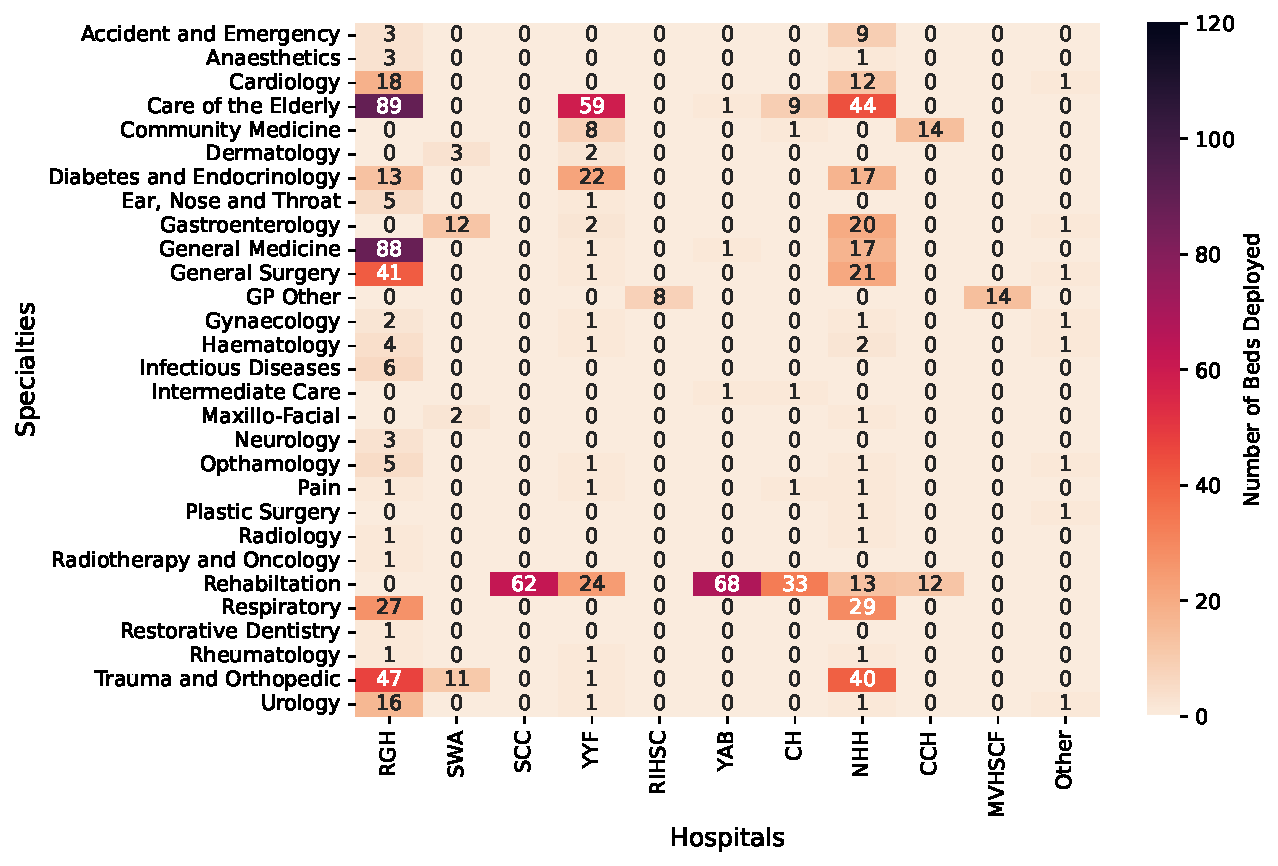
\includegraphics[scale=0.55]{Figures - Heatmaps/Fig1.pdf}
    \caption{Heatmap of bed locations for each specialty within each hospital for the deterministic model using the regression tree and average LOS over three years' worth of data.}
    \label{fig:app1}
\end{figure}

\begin{figure}
    \centering
    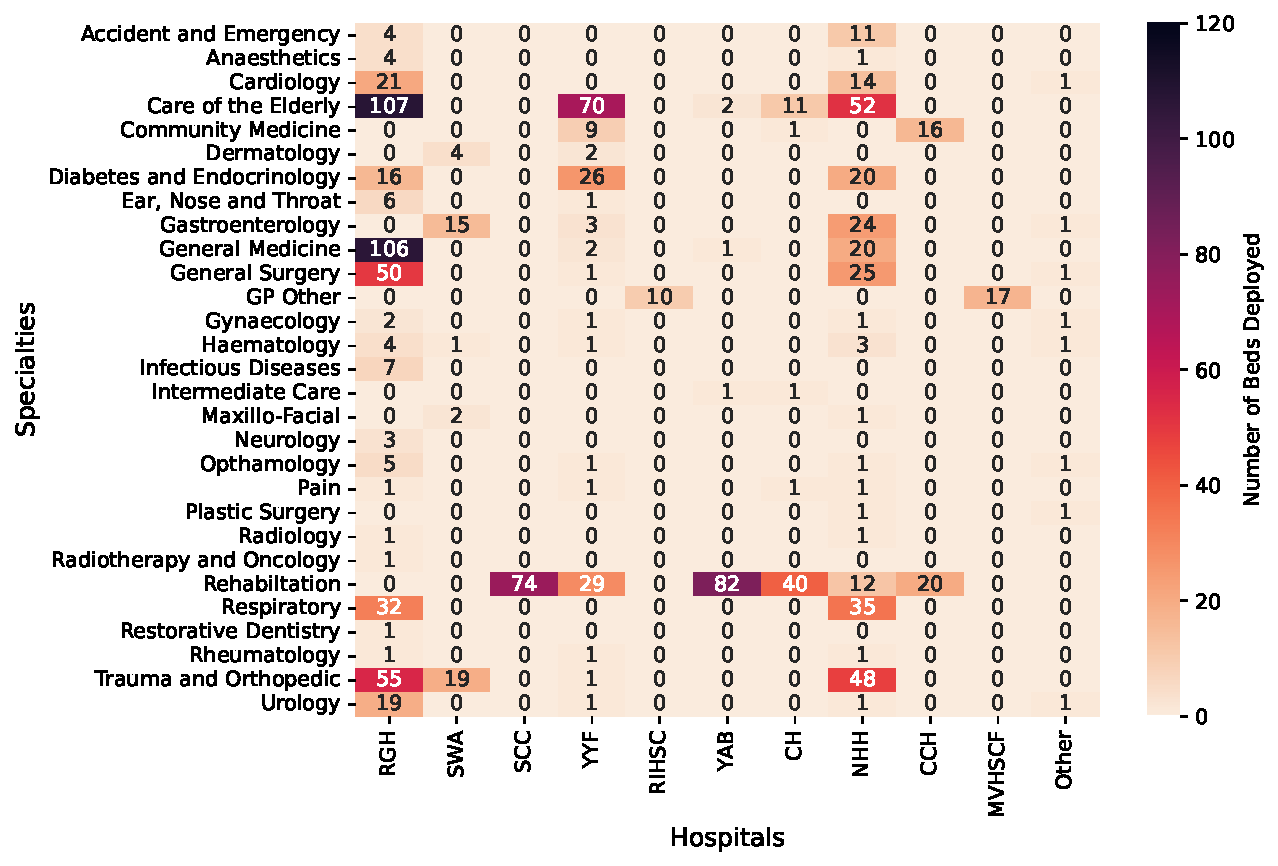
\includegraphics[scale=0.55]{Figures - Heatmaps/Fig2.pdf}
    \caption{Heatmap of bed locations for each specialty within each hospital for the two-stage stochastic model using the regression tree and average LOS over three years' worth of data.}
    \label{fig:app2}
\end{figure}

\begin{landscape}
\begin{table}[h!]
    \centering\scalebox{0.8}{
    \begin{tabular}{lcccccccccccccccccc}\toprule
\multirow{2}{*}{\textbf{Specialty}}& \multicolumn{3}{c}{\textbf{Region 1}} & \multicolumn{3}{c}{\textbf{Region 2}}& \multicolumn{3}{c}{\textbf{Region 3}}\\\cmidrule(lr){2-4} \cmidrule(lr){5-7}\cmidrule(lr){8-10}
& \textbf{2017-2018} & \textbf{2018-2019} & \textbf{2019-2020} & \textbf{2017-2018} & \textbf{2018-2019} & \textbf{2019-2020} & \textbf{2017-2018} & \textbf{2018-2019} & \textbf{2019-2020} \\\midrule
Accident \& Emergency&	3.2770	&3.3545&	2.2635&	0.0000	&0.0000&	0.0000	&0.0000&	0.0000	&0.0000\\
Anaesthetics &	2.8343&	2.3643&	2.6502&	0.0000&	0.0000&	0.0000&	0.0000&	0.0000&	0.0000\\
Cardiology &	17.0891&	16.0723&	19.2765&	0.0000&	0.0000&	0.0000&	0.0000&	0.0000&	0.0000\\
Care of the Elderly	&77.4710&	87.2786& 111.2406	&55.8412	&58.6116	&58.0388&	0.0000&	0.2651&	2.3439\\
Community Medicine	&0.0000&	0.0000	&0.0000&	6.6472&	6.8756&	7.8004	&0.0000&0.0000&	0.0000\\
Dermatology &	3.1669&	3.0209&	2.8880&	0.8694&	1.2436&	0.9720&	0.0000&	0.0000&	0.0000\\
Diabetes and Endocrinology	&14.1400&	10.1330	&13.5358	&25.2148&	20.3217&	19.6372&	0.0000&	0.0000&	0.0000\\
Ear Nose \& Throat	&4.6569&4.1676	&3.8168&0.0104&	0.0034	&0.0022	&0.0000&	0.0000&	0.0000\\
Gastroenterology &	11.7496&	9.1171&	14.1127&	2.0305&	1.8778&	1.9677&	0.0000&	0.0000&	0.0000\\
General Medicine&	104.7935	&98.2893&	59.7662&	0.3669	&0.8641&	1.6425&	0.0000&	0.0000&	0.0577\\
General Surgery	&41.4285&	41.4115&	39.3531	&0.5347&	0.7045&	1.2181&	0.0000	&0.0000&	0.0000\\
GP Other&	0.0000	&0.0000	&0.0000	&8.0565	&8.3022&	7.5475	&0.0000	&0.0000&	0.0000\\
Gynaecology &	1.6483&	1.3811&	1.8413&	0.1985&	0.0748&	0.0530&	0.0000&	0.0000&	0.0000\\
Haematology &	4.3233&	3.3572&	4.2947&	0.0000&	0.0000&	0.1845&	0.0000&	0.0000&	0.0000\\
Infectious Diseases&	6.3557&	5.0486&	4.9143&	0.0000&	0.0000&	0.0000&	0.0000&	0.0000&	0.0000\\
Intermediate Care&	0.0000&	0.0000&	0.0000&	0.0000&	0.0000&	0.0000&	0.0000&	0.0267&	0.6029\\
Maxillo-Facial&	1.3805&	1.3863&	0.9831&	0.0000&	0.0000&	0.0000&	0.0000&	0.0000&	0.0000\\
Neurology &	2.9267&	2.2129&	2.2365&	0.0000&	0.0000&	0.0000&	0.0000&	0.0000&	0.0000\\
Ophthalmology &	4.0896&	4.1329&	4.0669&	0.0000&	0.0000&	0.0360&	0.0000&	0.0000&	0.0000\\
Pain &	0.1175&	0.1290&	0.0938&	0.0000&	0.0235&	0.0099&	0.0000&	0.0000&	0.0000\\
Plastic Surgery&	0.0000&	0.0000&	0.0000&	0.0000&	0.0000&	0.0000&	0.0000&	0.0000&	0.0000\\
Radiology &	0.0069&	0.0311&	0.0313&	0.0000&	0.0000&	0.0000&	0.0000&	0.0000&	0.0000\\
Radiotherapy and Oncology&	0.0083&	0.0053&	0.0033&	0.0000&	0.0000&	0.0000&	0.0000&	0.0000&	0.0000\\
Rehabilitation &	64.8212&	60.5454&	60.3122&	34.5884&	34.4483&	29.0229&	69.0037&	64.8684&	72.0949\\
Respiratory &	28.3691&	26.0232&	24.8722&	0.0000&	0.0000&	0.0000&	0.0000&	0.0000&	0.0000\\
Restorative Dentistry&	0.0012&	0.0000&	0.0011&	0.0000&	0.0000&	0.0000&	0.0000&	0.0000&	0.0000\\
Rheumatology &	0.0000&	0.0000&	0.0011&	0.0000&	0.1473&	0.0000&	0.0000&	0.0000&	0.0000\\
Trauma and Orthopaedic&	57.1085&	59.2144&	57.0404&	0.3574&	0.4668&	0.2350&	0.0000&	0.0000&	0.0000\\
Urology &	14.0047&	15.9501&	15.2457&	0.1520&	0.1991&	0.0735&	0.0000&	0.0000&	0.0000\\
\bottomrule
\end{tabular}  } 
\caption{The daily bed demands for each specialty for regions one, two and three within ABUHB for three individual years’ worth of patient admissions, using the regression tree and average LOS.}
%\caption{Regions One, Two and Three Daily Demands for Three Individual Years of ABUHB Patient Admissions to Four Decimal Places - Regression Tree and Average LOS}
    \label{apptab:LinkedDemands2a}
\end{table}

\begin{table}[h!]
    \centering\scalebox{0.8}{
    \begin{tabular}{lcccccccccccccccccc}\toprule
\multirow{2}{*}{\textbf{Specialty}}& \multicolumn{3}{c}{\textbf{Region 4}} & \multicolumn{3}{c}{\textbf{Region 5}}& \multicolumn{3}{c}{\textbf{Region 6}}\\\cmidrule(lr){2-4} \cmidrule(lr){5-7}\cmidrule(lr){8-10}
& \textbf{2017-2018} & \textbf{2018-2019} & \textbf{2019-2020} & \textbf{2017-2018} & \textbf{2018-2019} & \textbf{2019-2020} & \textbf{2017-2018} & \textbf{2018-2019} & \textbf{2019-2020} \\\midrule

Accident \& Emergency&	0.0000&	0.0000&	0.0000&	7.6197&	8.9913	&8.8694&	0.0000&	0.0000&	0.0000\\
Anaesthetics&	0.0000&	0.0000&	0.0000&	0.3226&	0.3526&	0.7021&	0.0000&	0.0000&	0.0000\\
Cardiology&	0.0000&	0.0000&	0.0000&	14.1081&	11.6193&	9.3513&	0.0000&	0.0000&	0.0011\\
Care of the Elderly&	12.4192	&6.5233&	7.4180&	50.9444&	42.2170&	40.9048&	0.0000&	0.0000&	0.0000\\
Community Medicine	&0.4653&	0.1991&	0.4240&	15.5867&	14.5410&	9.9916&	0.0000&	0.0000&	0.0000\\
Dermatology&	0.0000&	0.0000&	0.0000&	0.0000&	0.0000&	0.0000&	0.0000&	0.0000&	0.0000\\
Diabetes and Endocrinology&	0.0000&	0.0000&	0.0000&	16.6930&	17.3699	&14.6714&	0.0000&	0.0000&	0.0000\\
Ear Nose \& Throat&	0.0000	&0.0000&	0.0000&	0.0000&	0.0000&	0.0000&	0.0000&	0.0000&	0.0000\\
Gastroenterology&	0.0000&	0.0000&	0.0000&	18.6975&	21.2773&	19.2673&	0.3178&	0.0000&	0.0022\\
General Medicine	&0.0000&	0.0000&	0.0000&	14.0661&	13.7832&	20.0969&	0.0000&	0.0000&	0.0000\\
General Surgery	&0.0000&	0.0000&	0.0000&	20.4384&	21.0748&	20.5769&	0.0012&	0.0011&	0.0011\\
GP Other	&0.0000&	0.0000&	0.0000&	15.5313&	12.5077&	14.4248&	0.0000&	0.0000&	0.0000\\
Gynaecology&	0.0000&	0.0000&	0.0000&	0.9696&	0.8862&	0.6536&	0.0000&	0.0000&	0.0011\\
Haematology&	0.0000&	0.0000&	0.0000&	1.8745&	1.7164&	1.5286&	0.0012&	0.0000&	0.0000\\
Infectious Diseases	&0.0000&	0.0000&	0.0000&	0.0000&	0.0000&	0.0000&	0.0000&	0.0000&	0.0000\\
Intermediate Care	&0.0000&	0.3300&	0.3561&	0.0000&	0.0000&	0.0000&	0.0000&	0.0000&	0.0000\\
Maxillo-Facial&	0.0000&	0.0000&	0.0000&	0.1129&	0.0761	&0.0971&	0.0000&	0.0000&	0.0000\\
Neurology&	0.0000&	0.0000&	0.0000&	0.0000&	0.0000&	0.0000&	0.0000&	0.0000&	0.0000\\
Opthamology&	0.0000&	0.0000&	0.0000&	0.4120&	0.4688&	0.4645&	0.0000&	0.9782&	1.2986\\
Pain&	0.0173&	0.0112&	0.0177&	0.0541&	0.0449&	0.0397&	0.0000&	0.0000&	0.0000\\
Plastic Surgery	&0.0000&	0.0000&	0.0000&	0.0548&	0.0471&	0.0463&	0.0000&	0.0000&	0.0011\\
Radiology&	0.0000&	0.0000&	0.0000&	0.0099&	0.0011&	0.0223&	0.0000&	0.0000&	0.0000\\
Radiotherapy and Oncology&	0.0000&	0.0000&	0.0000&	0.0000&	0.0000	&0.0000&	0.0000&	0.0000&	0.0000\\
Rehabilitation&	29.8605&	35.5390&	33.8379&	18.3697&	25.2679&	28.8564&	0.0000&	0.0000&	0.0000\\
Respiratory&	0.0000&	0.0000&	0.0000&	32.6054&	28.9470&	24.7762&	0.0000&	0.0000&	0.0000\\
Restorative Dentistry	&0.0000&	0.0000&	0.0000&	0.0000&	0.0000&	0.0000&	0.0000&	0.0000&	0.0000\\
Rheumatology&	0.0000&	0.0000&	0.0000&	0.0000&	0.0214&	0.0000&	0.0000&	0.0000&	0.0000\\
Trauma and Orthopedic&	0.0000&	0.0000&	0.0000&	37.1555&	40.9789	&40.7325&	0.0000&	0.0000&	0.0000\\
Urology&	0.0000&	0.0000&	0.0000&	0.5282&	0.5165&	0.4400&	0.0219&	0.0181&	0.0184\\
\bottomrule


\end{tabular}  } 
\caption{The daily bed demands for each specialty for regions four, five and six within ABUHB for three individual years’ worth of patient admissions, using the regression tree and average LOS.}
    \label{apptab:LinkedDemands2b}
\end{table}

\begin{figure}[h!]
\centering
\begin{minipage}{0.4\linewidth}
  \centering
  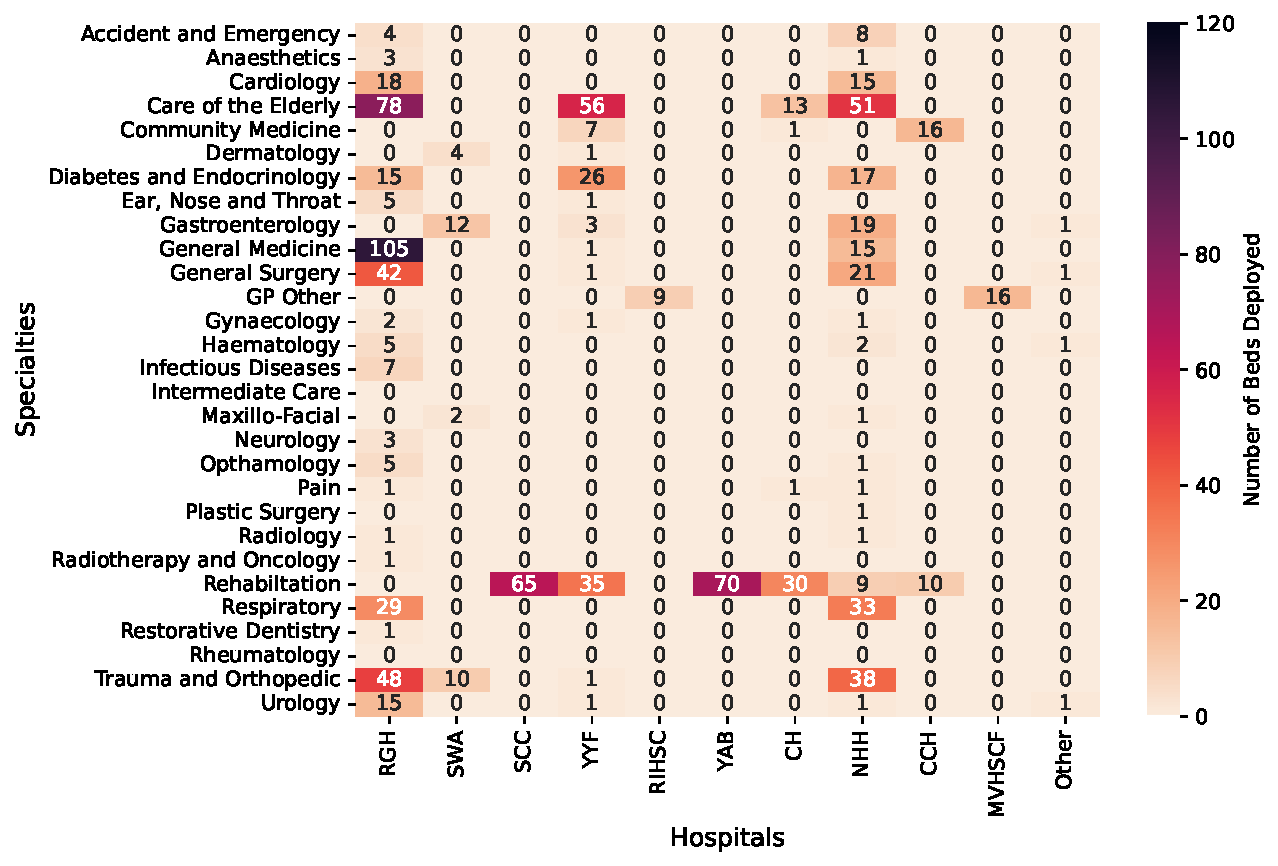
\includegraphics[scale=0.4]{Figures - Heatmaps/Fig3.pdf}
  \captionsetup{font={scriptsize}}
  \captionof{figure}{{Heatmap of bed locations for each specialty within each\\ hospital for the deterministic model using the regression tree and \\average LOS for 2017-2018.}}
  \label{fig:app3a}
\end{minipage}%
\
\begin{minipage}{0.4\linewidth}
  \centering
  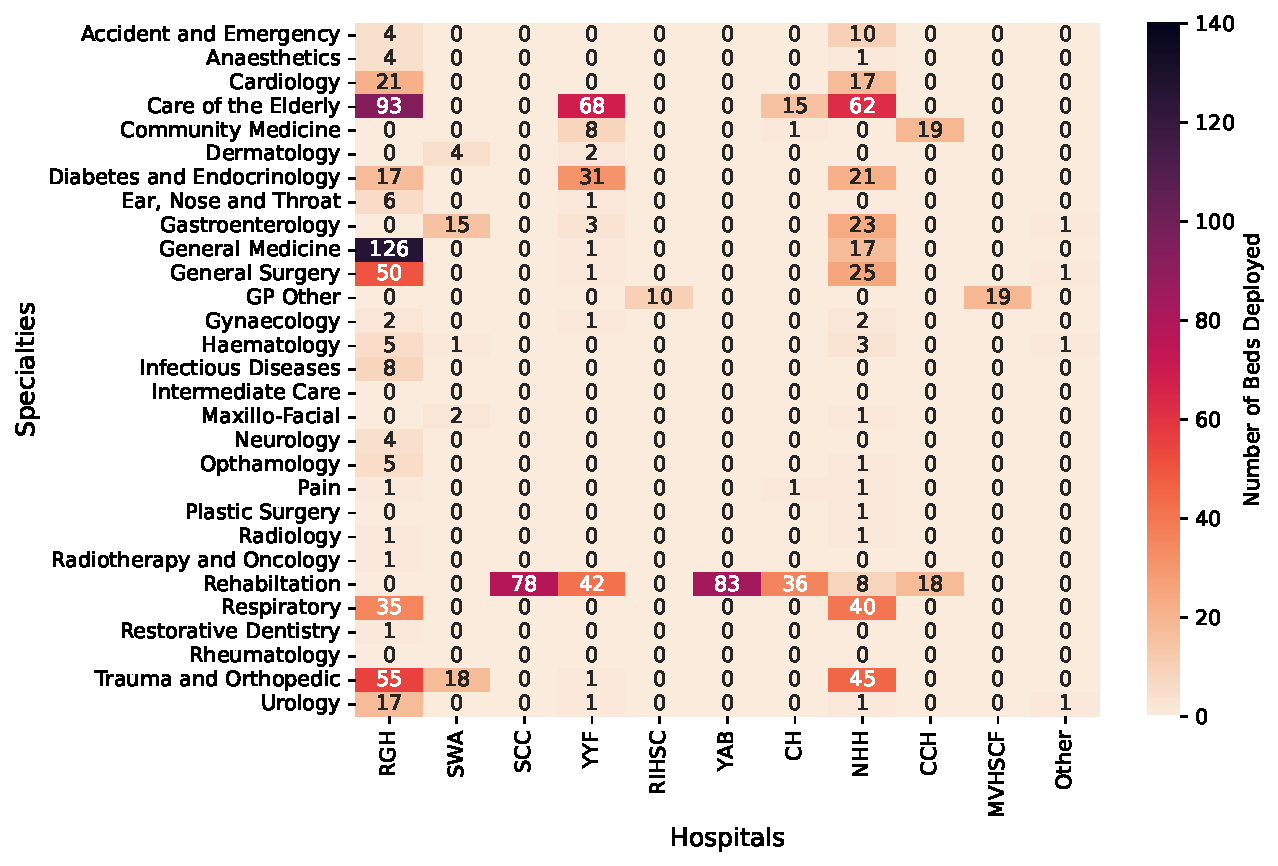
\includegraphics[scale=0.4]{Figures - Heatmaps/Fig4.pdf}  \captionsetup{font={scriptsize}}
  \captionof{figure}{Heatmap of bed locations for each specialty within each\\ hospital for the two-stage stochastic model using the regression tree and \\average LOS for 2017-2018.}
  \label{fig:app3b}
\end{minipage}
\end{figure}

\begin{figure}[h!]
\centering
\begin{minipage}{0.4\linewidth}
  \centering
  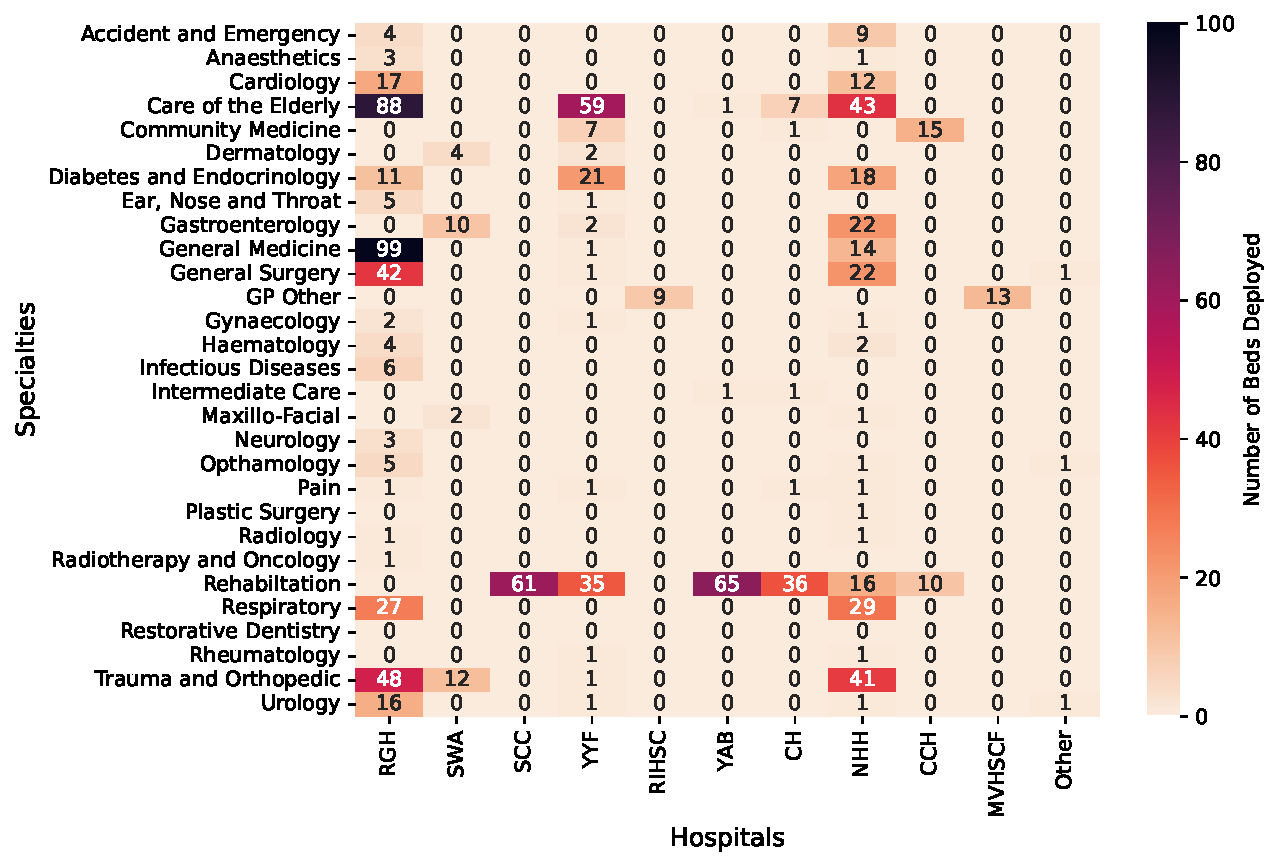
\includegraphics[scale=0.4]{Figures - Heatmaps/Fig5.pdf}
\captionsetup{font={scriptsize}}
  \captionof{figure}{{Heatmap of bed locations for each specialty within each\\ hospital for the deterministic model using the regression tree and \\average LOS for 2018-2019.}}
  \label{fig:app4a}
\end{minipage}%
\begin{minipage}{0.4\linewidth}
  \centering
  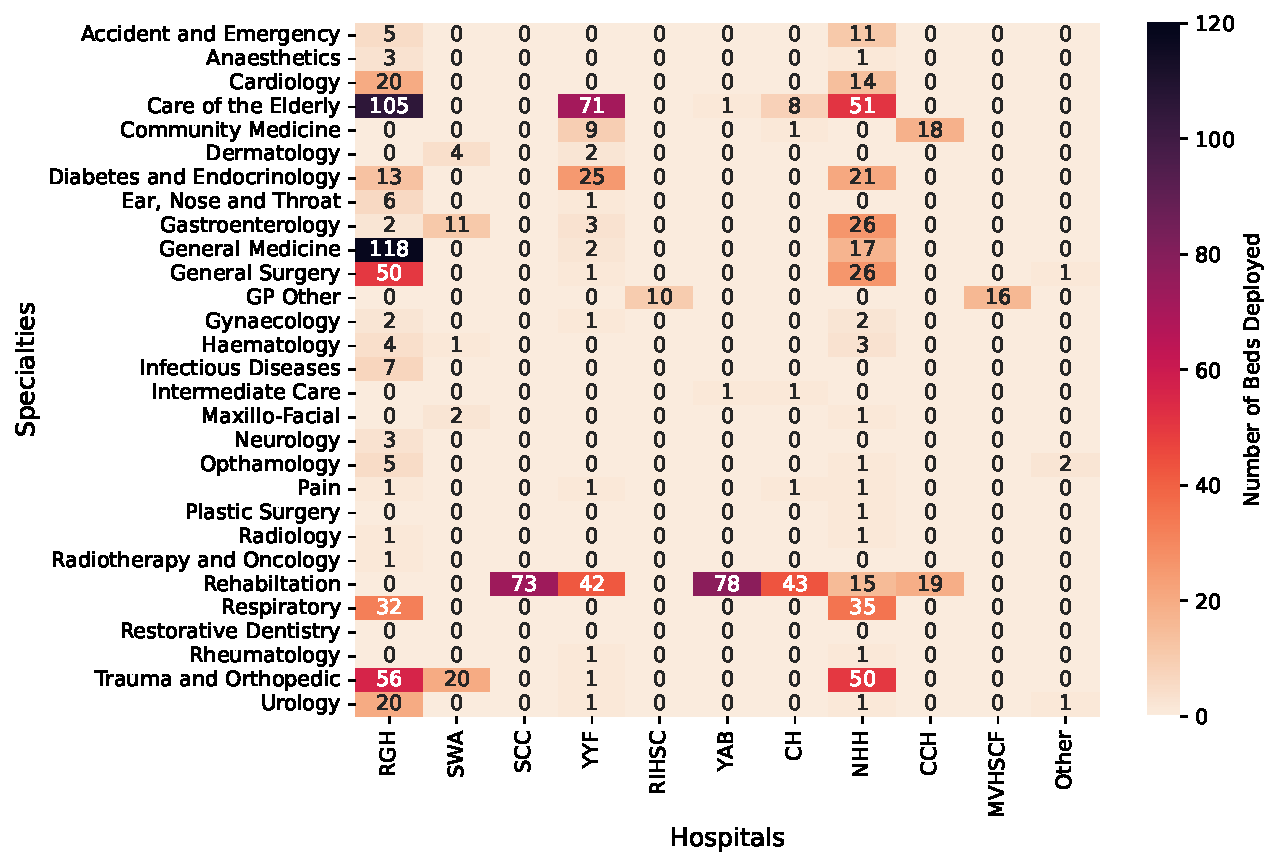
\includegraphics[scale=0.4]{Figures - Heatmaps/Fig6.pdf}
  \captionsetup{font={scriptsize}}
  \captionof{figure}{{Heatmap of bed locations for each specialty within each\\ hospital for the two-stage stochastic model using the regression tree and \\average LOS for 2018-2019.}}
  \label{fig:app4b}
\end{minipage}
\end{figure}

\begin{figure}[h!]
\centering
\begin{minipage}{0.4\linewidth}
  \centering
  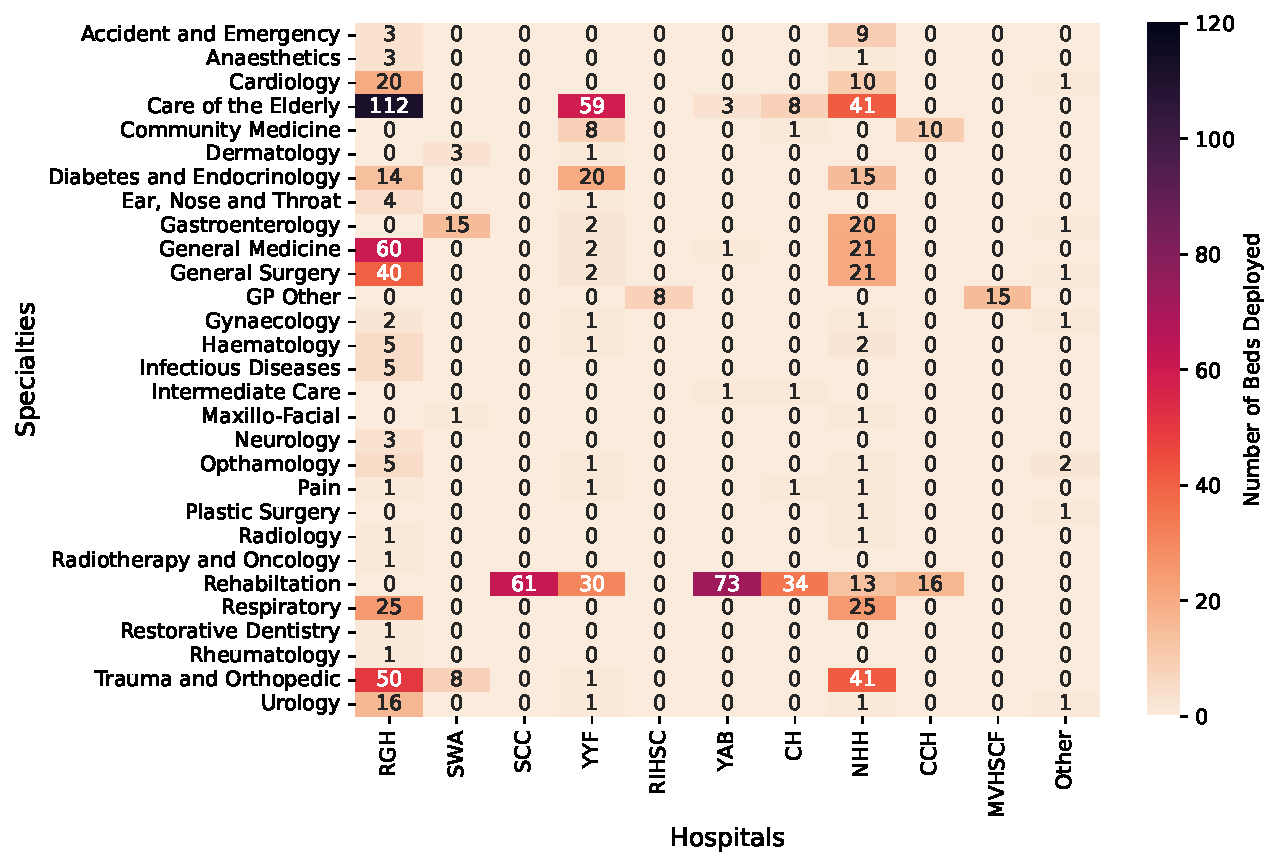
\includegraphics[scale=0.4]{Figures - Heatmaps/Fig7.pdf}
\captionsetup{font={scriptsize}}
  \captionof{figure}{{Heatmap of bed locations for each specialty within each\\ hospital for the deterministic model using the regression tree and \\average LOS for 2019-2020.}}
  \label{fig:app5a}
\end{minipage}%
\begin{minipage}{0.4\linewidth}
  \centering
  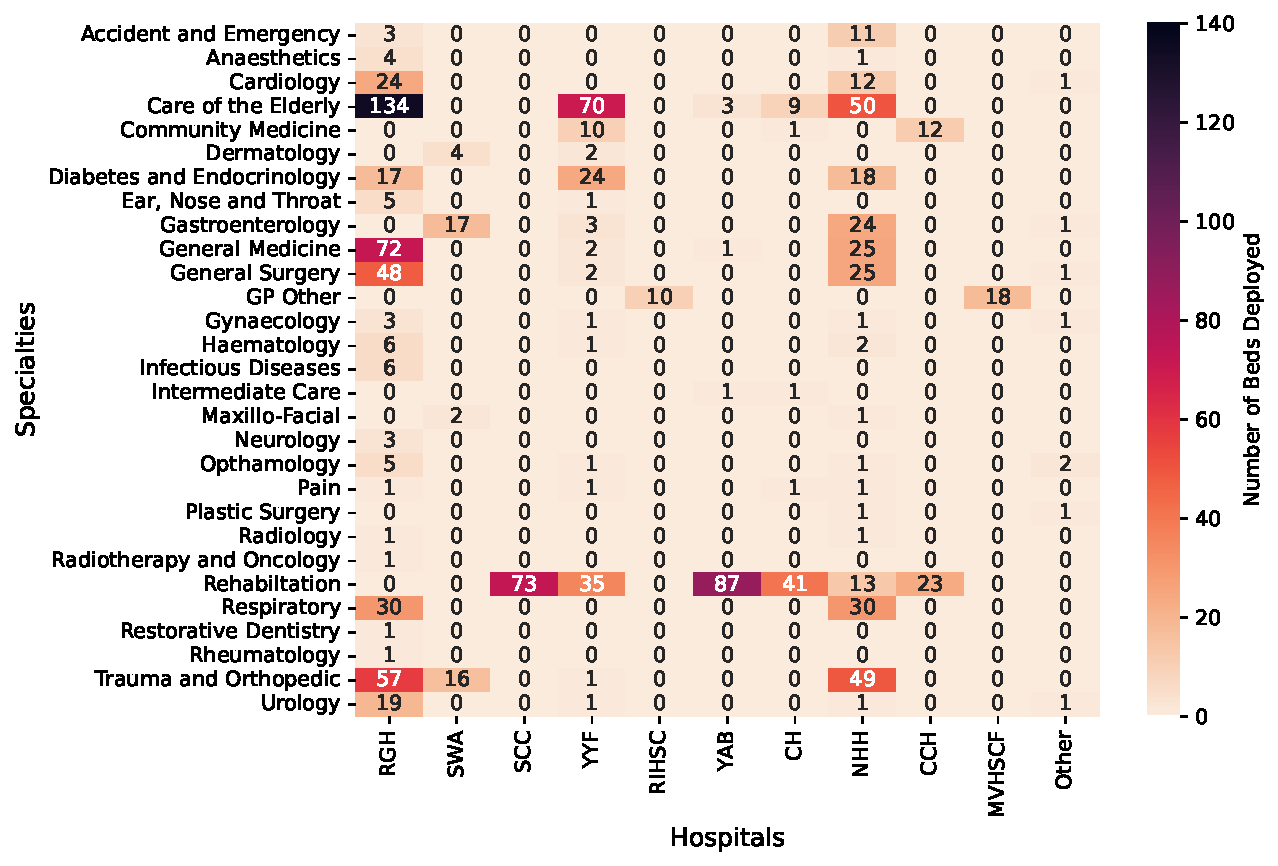
\includegraphics[scale=0.4]{Figures - Heatmaps/Fig8.pdf}
  \captionsetup{font={scriptsize}}
  \captionof{figure}{{Heatmap of bed locations for each specialty within each\\ hospital for the two-stage stochastic model using the regression tree and \\average LOS for 2019-2020.}}
  \label{fig:app5b}
\end{minipage}
\end{figure}
% \begin{minipage}[c]{0.4\linewidth}
%         \begin{figure}[h!]
%             \centering
%             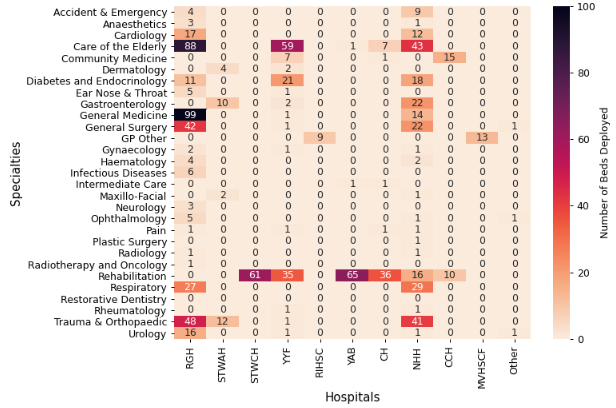
\includegraphics[width=.48\linewidth]{Chapters/Figures - Appendix/App4a.png}
%             \caption{Number of patients waiting up to 26 weeks in Wales (Jan. `18 - Aug. `22).}
%         \end{figure}
%     \end{minipage}\hspace{1cm}
%     \begin{minipage}[c]{0.4\linewidth}
%         \begin{figure}[h!]
%             \centering
%             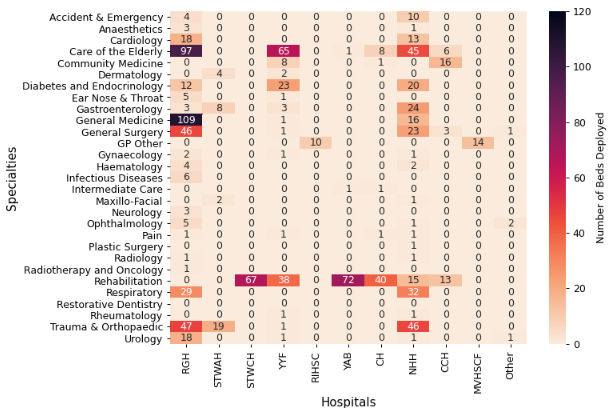
\includegraphics[width=.48\linewidth]{Chapters/Figures - Appendix/App4b.png}
%             \caption{Number of patients waiting over 36 weeks in Wales (Jan. `18 - Aug. `22).}
%         \end{figure}
%     \end{minipage}
    
% \begin{figure*}[t!]
%         \subfloat[A Cap]{%
%             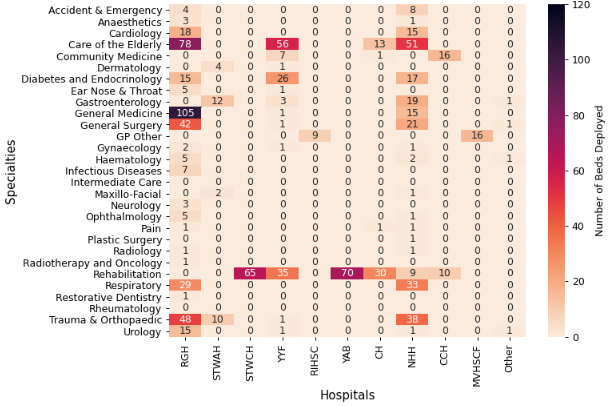
\includegraphics[width=.48\linewidth]{Chapters/Figures - Appendix/App3a.png}%
%             \label{subfig:a}%
%         }\hfill
%         \subfloat[B Cap]{%
%             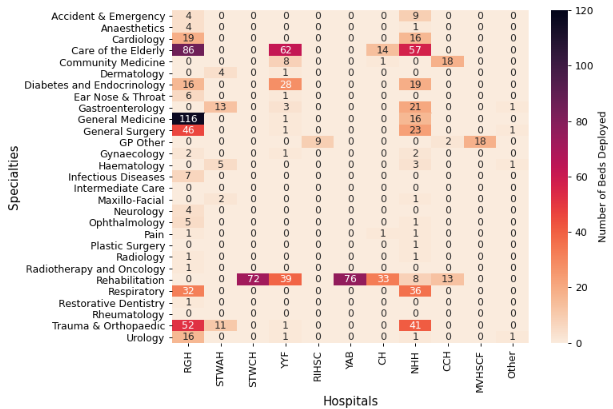
\includegraphics[width=.48\linewidth]{Chapters/Figures - Appendix/App3b.png}%
%             \label{subfig:b}%
%         }\\
%         \subfloat[C Cap]{%
%             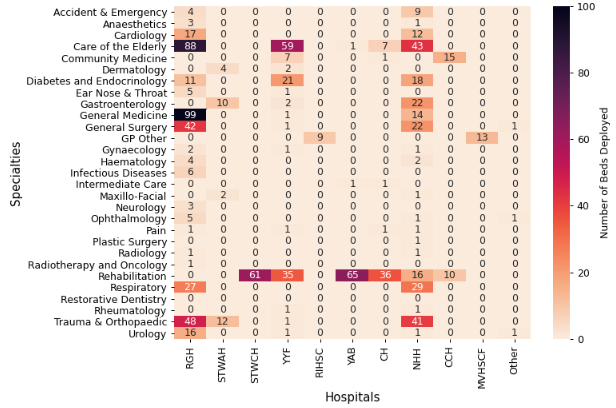
\includegraphics[width=.48\linewidth]{Chapters/Figures - Appendix/App4a.png}%
%             \label{subfig:c}%
%         }\hfill
%         \subfloat[D Cap]{%
%             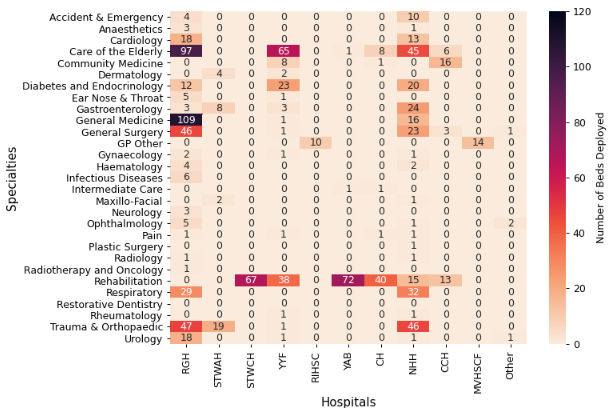
\includegraphics[width=.48\linewidth]{Chapters/Figures - Appendix/App4b.png}%
%             \label{subfig:d}%

%         }
%         \caption{Caption}
%         \label{fig:fig}
% \end{figure*}
\end{landscape}




\begin{landscape}
    \begin{table}[h!]
    \centering\scalebox{0.8}{
    \begin{tabular}{lcccccccccccccccccc}\toprule
\multirow{2}{*}{\textbf{Specialty}}& \multicolumn{3}{c}{\textbf{Region 1}} & \multicolumn{3}{c}{\textbf{Region 2}}& \multicolumn{3}{c}{\textbf{Region 3}}\\\cmidrule(lr){2-4} \cmidrule(lr){5-7}\cmidrule(lr){8-10}
& \textbf{2017-2018} & \textbf{2018-2019} & \textbf{2019-2020} & \textbf{2017-2018} & \textbf{2018-2019} & \textbf{2019-2020} & \textbf{2017-2018} & \textbf{2018-2019} & \textbf{2019-2020} \\\midrule

Accident \& Emergency&	3.2862&	3.1969&	2.4505&	0.0000&	0.0000&	0.0000&	0.0000&	0.0000&	0.0000\\
Anaesthetics	&2.7907&	2.3695&	2.6954&	0.0000&	0.0000&	0.0000&	0.0000&	0.0000&	0.0000\\
Cardiology	&16.9908&	15.9287&	19.5686&	0.0000&	0.0000&	0.0000&	0.0000&	0.0000&	0.0000\\
Care of the Elderly&	86.2987&	101.7951&	124.1676&	56.7726&	59.3095&	57.9663&	0.0000&	0.2609&	2.6423\\
Community Medicine	&0.0000&	0.0000&	0.0000&	6.2182&	7.2636&	7.7736&	0.0000&	0.0000&	0.0000\\
Dermatology	&2.9946&	3.0185&	2.8964&	0.8336&	1.2245&	0.9701&	0.0000&	0.0000&	0.0000\\
Diabetes and Endocrinology&	13.8852&	10.2042&	13.9090&	23.7736&	20.7721&	20.4075&	0.0000&	0.0000&	0.0000\\
Ear Nose \& Throat&	4.5786&	4.1889&	3.9077&	0.0099&	0.0033&	0.0022&	0.0000&	0.0000&	0.0000\\
Gastroenterology	&11.5280&	9.1310&	14.4347&	1.9533&	1.8463&	1.9979&	0.0000&	0.0000&	0.0000\\
General Medicine	&102.9001&	99.0452&	61.3219&	0.3693&	0.8681&	1.6574&	0.0000&	0.0000&	0.0650\\
General Surgery	&40.7516&	42.1739&	40.0680&	0.5145&	0.6929&	1.2279&	0.0000&	0.0000&	0.0000\\
GP Other	&0.0000&	0.0000&	0.0000&	7.3663&	8.8037&	7.5505&	0.0000&	0.0000&	0.0000\\
Gynaecology	&1.6100&	1.3820&	1.8843&	0.1921&	0.0735&	0.0529&	0.0000&	0.0000&	0.0000\\
Haematology	&4.1320&	3.3443&	4.3536&	0.0000&	0.0000&	0.1950&	0.0000&	0.0000&	0.0000\\
Infectious Diseases	&6.2340&	5.0822&	5.0511&	0.0000&	0.0000&	0.0000&	0.0000&	0.0000&	0.0000\\
Intermediate Care	&0.0000&	0.0000&	0.0000&	0.0000&	0.0000&	0.0000&	0.0000&	0.0269&	0.6293\\
Maxillo-Facial&	1.3366&	1.3814&	0.9905&	0.0000&	0.0000&	0.0000&	0.0000&	0.0000&	0.0000\\
Neurology	&2.8786&	2.2274&	2.2958&	0.0000&	0.0000&	0.0000&	0.0000&	0.0000&	0.0000\\
Ophthalmology	&3.9421&	4.0835&	4.0948&	0.0000&	0.0000&	0.0367&	0.0000&	0.0000&	0.0000\\
Pain	&0.1126&	0.1268&	0.0936&	0.0000&	0.0232&	0.0099&	0.0000&	0.0000&	0.0000\\
Plastic Surgery	&0.0000&	0.0000&	0.0000&	0.0000&	0.0000&	0.0000&	0.0000&	0.0000&	0.0000\\
Radiology	&0.0066&	0.0313&	0.0318&	0.0000&	0.0000&	0.0000&	0.0000&	0.0000&	0.0000\\
Radiotherapy and Oncology&	0.0061&	0.0049&	0.0033&	0.0000&	0.0000&	0.0000&	0.0000&	0.0000&	0.0000\\
Rehabilitation	&64.1492&	56.7391&	63.4545&	24.5786&	25.2688&	21.4197&	58.7946&	63.8572&	81.1403\\
Respiratory	&27.8692&	26.1755&	25.5186&	0.0000&	0.0000&	0.0000&	0.0000&	0.0000&	0.0000\\
Restorative Dentistry	&0.0011&	0.0000&	0.0011&	0.0000&	0.0000&	0.0000&	0.0000&	0.0000&	0.0000\\
Rheumatology	&0.0000&	0.0000&	0.0011&	0.0000&	0.1473&	0.0000&	0.0000&	0.0000&	0.0000\\
Trauma \& Orthopaedic&	54.3186&	62.5405&	56.4987&	0.3162&	0.4968&	0.2410&	0.0000&	0.0000&	0.0000\\
Urology	&13.6899&	15.8597&	16.0522&	0.1457&	0.1941&	0.0963&	0.0000&	0.0000&	0.0000\\

\bottomrule
\end{tabular}  } 
\caption{The daily bed demands for each specialty for regions one, two and three within ABUHB for three individual years’ worth of patient admissions, using the regression tree and the year specific average LOS.}
%\caption{Regions One, Two and Three Daily Demands for Three Individual Years of ABUHB Patient Admissions to Four Decimal Places - Regression Tree and Year Specific Average LOS}
    \label{apptab:LinkedDemands3a}
\end{table}

\begin{table}[h!]
    \centering\scalebox{0.8}{
    \begin{tabular}{lcccccccccccccccccc}\toprule
\multirow{2}{*}{\textbf{Specialty}}& \multicolumn{3}{c}{\textbf{Region 4}} & \multicolumn{3}{c}{\textbf{Region 5}}& \multicolumn{3}{c}{\textbf{Region 6}}\\\cmidrule(lr){2-4} \cmidrule(lr){5-7}\cmidrule(lr){8-10}
& \textbf{2017-2018} & \textbf{2018-2019} & \textbf{2019-2020} & \textbf{2017-2018} & \textbf{2018-2019} & \textbf{2019-2020} & \textbf{2017-2018} & \textbf{2018-2019} & \textbf{2019-2020} \\\midrule

Accident \& Emergency&	0.0000&	0.0000&	0.0000&	7.6680&	8.6804&	9.9681&	0.0000&	0.0000&	0.0000\\
Anaesthetics&	0.0000&	0.0000&	0.0000&	0.4638&	0.4268&	0.9722&	0.0000&	0.0000&	0.0000\\
Cardiology&	0.0000&	0.0000&	0.0000&	16.1539&	14.2806&	11.1400&	0.0000&	0.0000&	0.0011\\
Care of the Elderly&	12.5281&	6.5938&	6.8223&	52.3094&	45.1508&	41.2107&	0.0000&	0.0000&	0.0000\\
Community Medicine	&0.4234&	0.2117&	0.4222&	14.1831&	15.4549&	9.9576&	0.0000&	0.0000&	0.0000\\
Dermatology&	0.0000&	0.0000&	0.0000&	0.0000&	0.0000&	0.0000&	0.0000&	0.0000&	0.0000\\
Diabetes and Endocrinology&	0.0000&	0.0000&	0.0000&	16.6698&	17.8823&	15.3511&	0.0000&	0.0000&	0.0000\\
Ear Nose \& Throat&	0.0000&	0.0000&	0.0000&	0.0000&	0.0000&	0.0000&	0.0000&	0.0000&	0.0000\\
Gastroenterology&	0.0000&	0.0000&	0.0000&	18.7998&	21.9374&	19.9778&	0.3047&	0.0000&	0.0022\\
General Medicine	&0.0000&	0.0000&	0.0000&	13.9936&	14.0130&	20.9445&	0.0000&	0.0000&	0.0000\\
General Surgery	&0.0000&	0.0000&	0.0000&	20.4583&	21.6905&	21.4020&	0.0011&	0.0011&	0.0011\\
GP Other	&0.0000&	0.0000&	0.0000&	14.1544&	13.2848&	14.3738&	0.0000&	0.0000&	0.0000\\
Gynaecology&	0.0000&	0.0000&	0.0000&	0.9738&	0.9246&	0.6943&	0.0000&	0.0000&	0.0011\\
Haematology&	0.0000&	0.0000&	0.0000&	1.8249&	1.7582&	2.0842&	0.0011&	0.0000&	0.0000\\
Infectious Diseases	&0.0000&	0.0000&	0.0000&	0.0000&	0.0000&	0.0000&	0.0000&	0.0000&	0.0000\\
Intermediate Care	&0.0000&	0.3333&	0.3699&	0.0000&	0.0000&	0.0000&	0.0000&	0.0000&	0.0000\\
Maxillo-Facial&	0.0000	&0.0000	&0.0000&	0.1061	&0.0747&	0.0969&	0.0000	&0.0000&	0.0000\\
Neurology&	0.0000&	0.0000&	0.0000&	0.0000&	0.0000&	0.0000&	0.0000&	0.0000&	0.0000\\
Ophthalmology&	0.0000&	0.0000&	0.0000&	0.3948&	0.4613&	0.4636&	0.0000&	0.9640&	1.2960\\
Pain&	0.0166&	0.0110&	0.0176&	0.0519&	0.0442&	0.0396&	0.0000&	0.0000&	0.0000\\
Plastic Surgery	&0.0000&	0.0000&	0.0000&	0.0521&	0.0464&	0.0462&	0.0000&	0.0000&	0.0011\\
Radiology&	0.0000&	0.0000&	0.0000&	0.0091&	0.0011&	0.0225&	0.0000&	0.0000&	0.0000\\
Radiotherapy and Oncology&	0.0000&	0.0000&	0.0000&	0.0000&	0.0000&	0.0000&	0.0000&	0.0000&	0.0000\\
Rehabilitation&	29.5478&	33.4318&	35.5989&	10.7206&	16.2437&	23.0764&	0.0000&	0.0000&	0.0000\\
Respiratory&	0.0000&	0.0000&	0.0000&	32.7445&	29.8673&	25.8748&	0.0000&	0.0000&	0.0000\\
Restorative Dentistry	&0.0000&	0.0000&	0.0000&	0.0000&	0.0000&	0.0000&	0.0000&	0.0000&	0.0000\\
Rheumatology&	0.0000&	0.0000&	0.0000&	0.0000&	0.0215&	0.0000&	0.0000&	0.0000&	0.0000\\
Trauma \& Orthopaedic&	0.0000&	0.0000&	0.0000&	36.3659&	44.0053&	41.3888&	0.0000&	0.0000&	0.0000\\
Urology&	0.0000&	0.0000&	0.0000&	0.5179&	0.4967&	0.5494&	0.0210&	0.0169&	0.0226\\


\bottomrule


\end{tabular}  } 
\caption{The daily bed demands for each specialty for regions four, five and six within ABUHB for three individual years’ worth of patient admissions, using the regression tree and the year specific average LOS.}
    \label{apptab:LinkedDemands3b}
\end{table}


\begin{figure}[h!]
\centering
\begin{minipage}{0.4\linewidth}
  \centering
  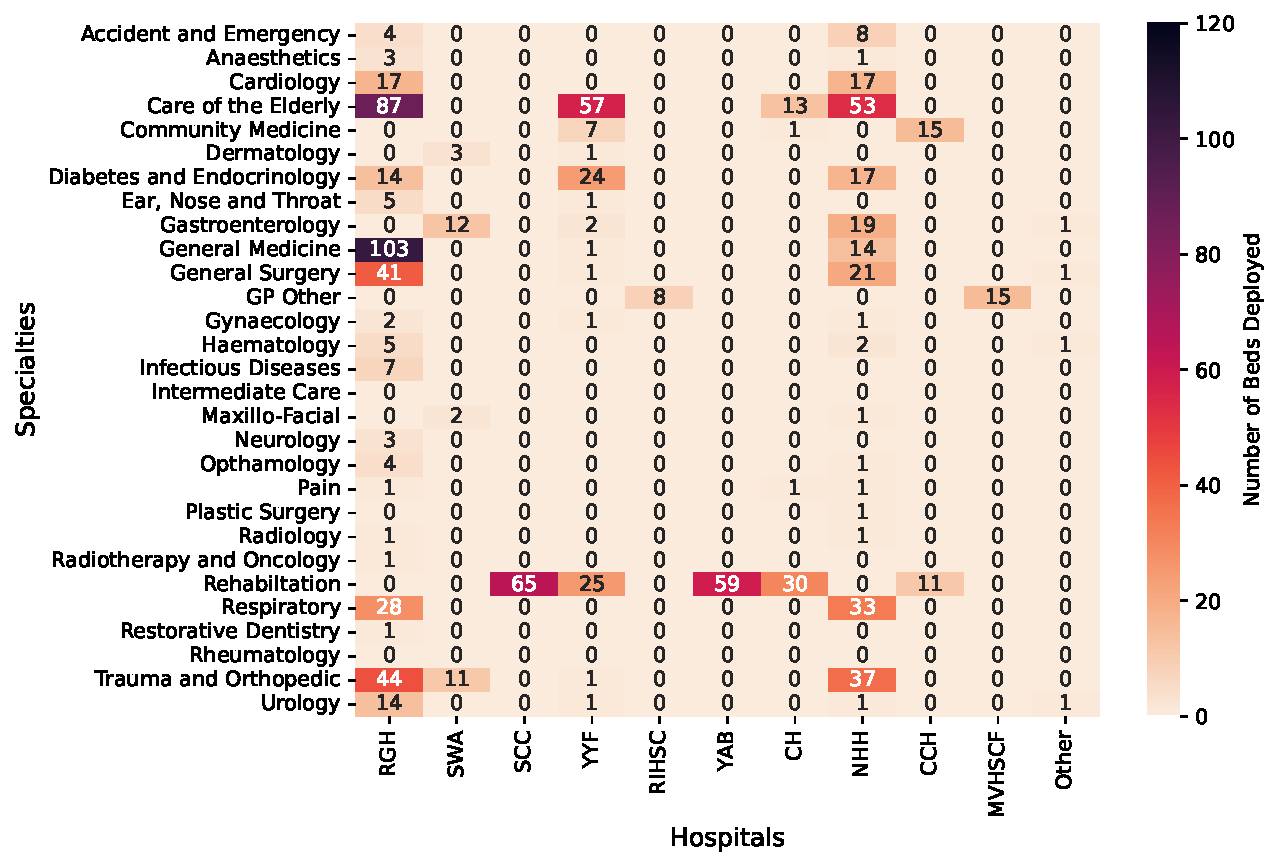
\includegraphics[scale=0.4]{Figures - Heatmaps/Fig9.pdf}
  \captionsetup{font={scriptsize}}
  \captionof{figure}{{Heatmap of bed locations for each specialty within each\\ hospital for the deterministic model using the regression tree and \\average year LOS for 2017-2018.}}
 % \captionof{figure}{{Heatmap of Bed Locations for Each Specialty within Each\\ Hospital - Deterministic Results - Regression Tree and Average Year LOS - \\2017-2018}}
  \label{fig:app7a}
\end{minipage}%
\begin{minipage}{0.4\linewidth}
  \centering
  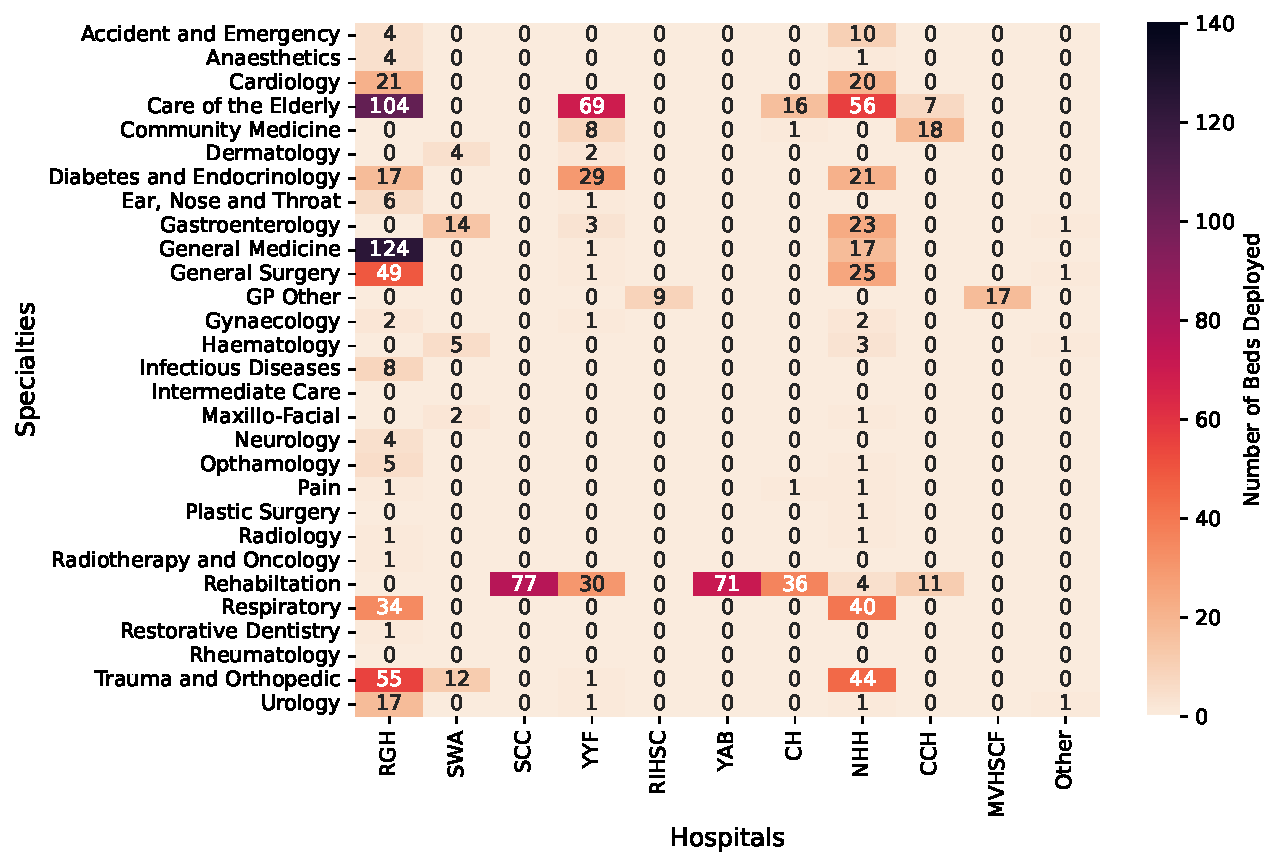
\includegraphics[scale=0.4]{Figures - Heatmaps/Fig10.pdf}  \captionsetup{font={scriptsize}}
  \captionof{figure}{{Heatmap of bed locations for each specialty within each\\ hospital for the two-stage stochastic model using the regression tree and \\average year LOS for 2017-2018.}}
  \label{fig:app7b}
\end{minipage}
\end{figure}

\begin{figure}[h!]
\centering
\begin{minipage}{0.4\linewidth}
  \centering
  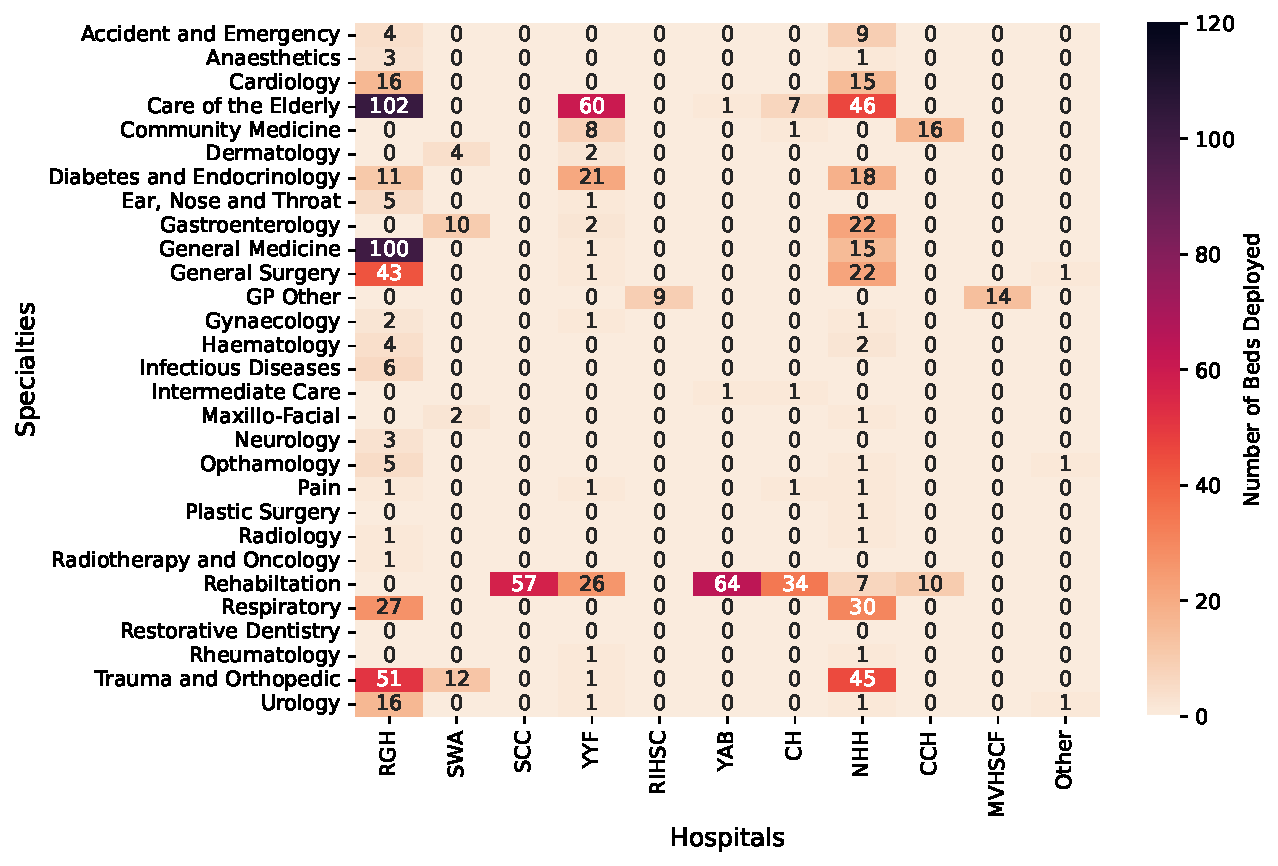
\includegraphics[scale=0.4]{Figures - Heatmaps/Fig11.pdf}
\captionsetup{font={scriptsize}}
  \captionof{figure}{{Heatmap of bed locations for each specialty within each\\ hospital for the deterministic model using the regression tree and \\average year LOS for 2018-2019.}}
  \label{fig:app8a}
\end{minipage}%
\begin{minipage}{0.4\linewidth}
  \centering
  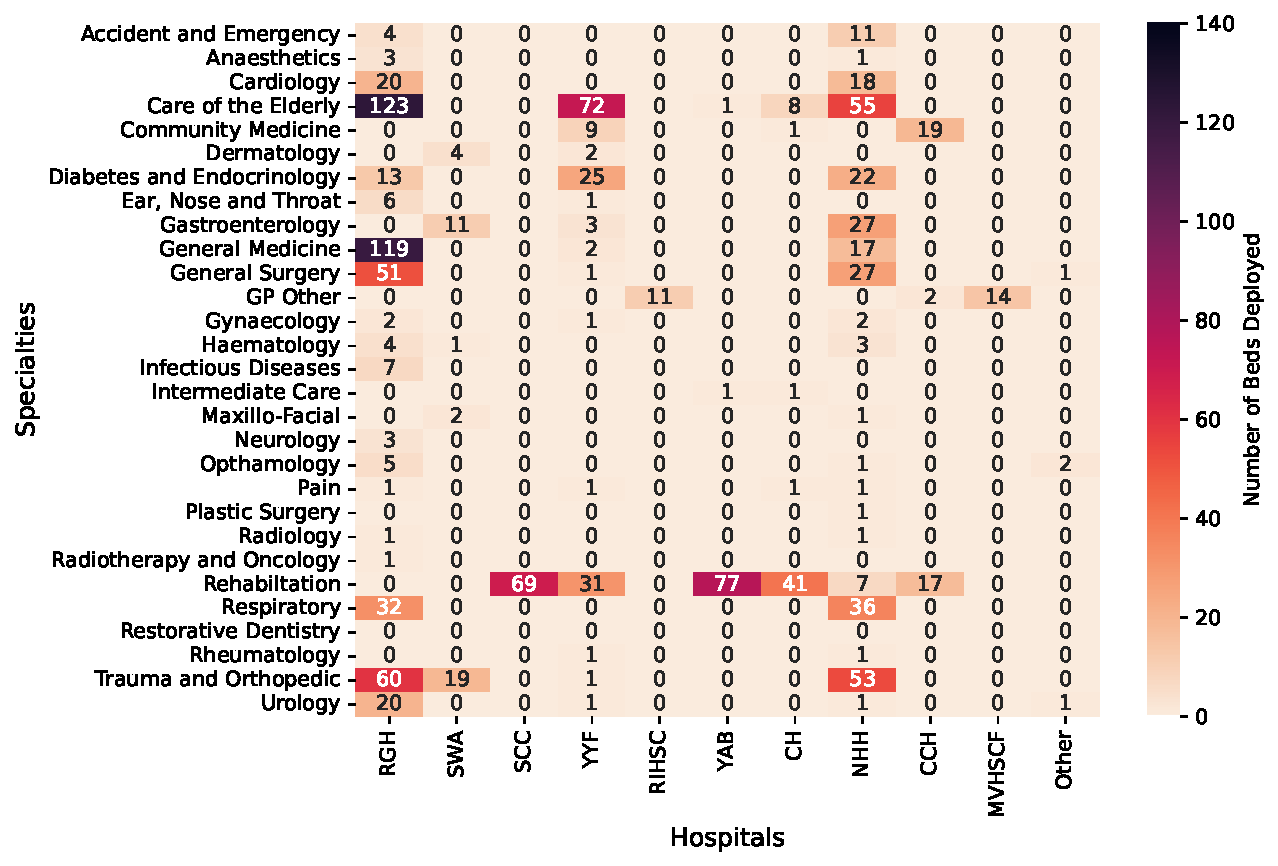
\includegraphics[scale=0.4]{Figures - Heatmaps/Fig12.pdf}
  \captionsetup{font={scriptsize}}
  \captionof{figure}{{Heatmap of bed locations for each specialty within each\\ hospital for the two-stage stochastic model using the regression tree and \\average year LOS for 2018-2019.}}
  \label{fig:app8b}
\end{minipage}
\end{figure}

\begin{figure}[h!]
\centering
\begin{minipage}{0.4\linewidth}
  \centering
  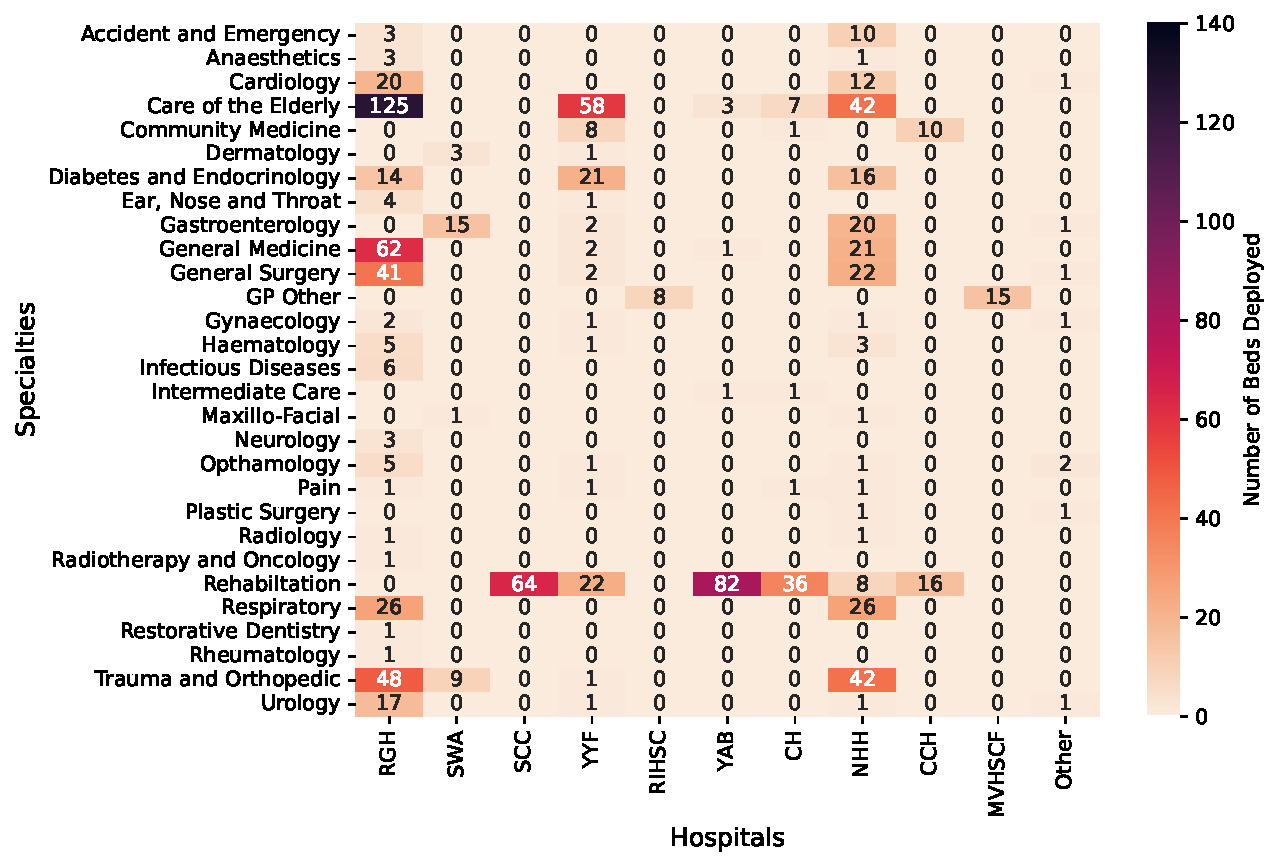
\includegraphics[scale=0.4]{Figures - Heatmaps/Fig13.pdf}
\captionsetup{font={scriptsize}}
  \captionof{figure}{{Heatmap of bed locations for each specialty within each\\ hospital for the deterministic model using the regression tree and \\average year LOS for 2019-2020.}}
  \label{fig:app9a}
\end{minipage}%
\begin{minipage}{0.4\linewidth}
  \centering
  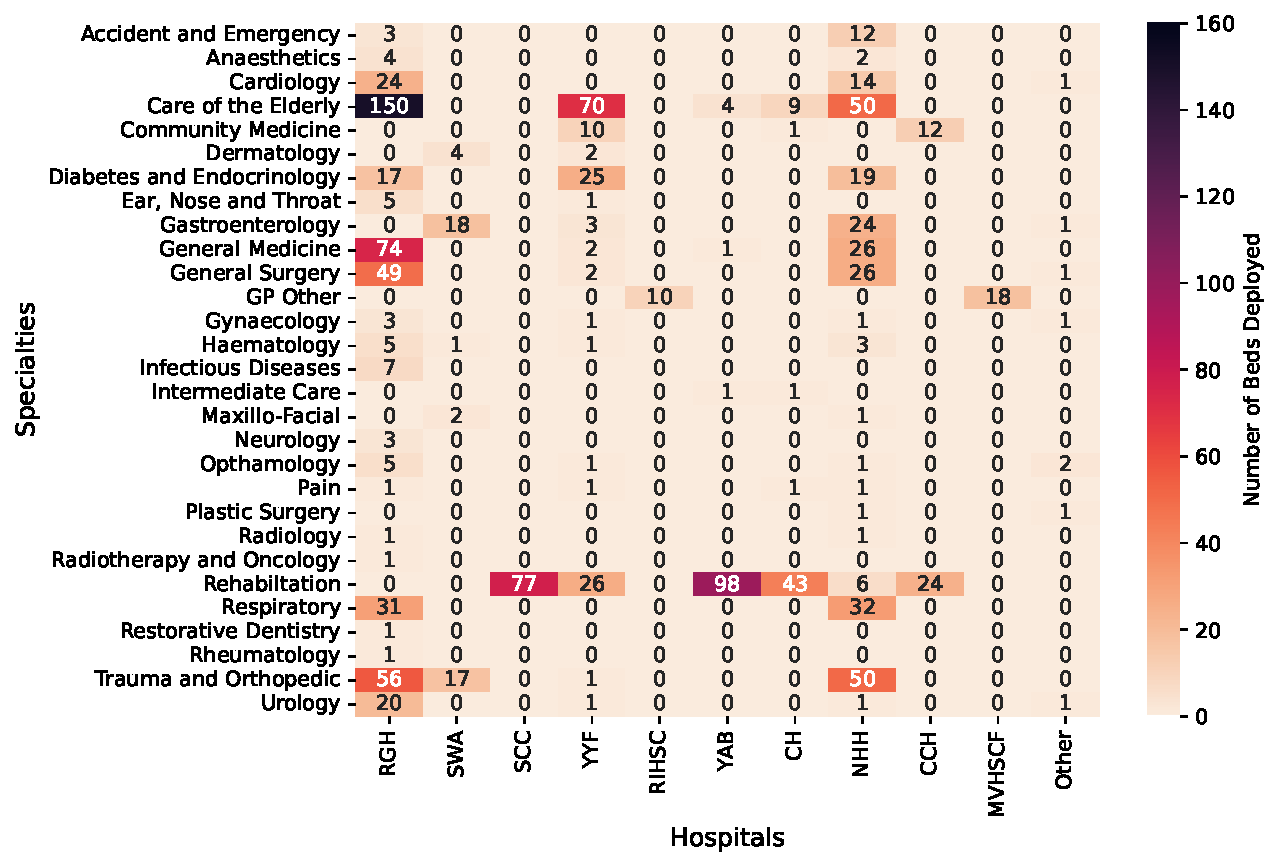
\includegraphics[scale=0.4]{Figures - Heatmaps/Fig14.pdf}
  \captionsetup{font={scriptsize}}
  \captionof{figure}{{Heatmap of bed locations for each specialty within each\\ hospital for the two-stage stochastic model using the regression tree and \\average year LOS for 2019-2020.}}
  \label{fig:app9b}
\end{minipage}
\end{figure}
\end{landscape}
\section{Regression Trees - Specific LOS}
\begin{table}[h!]
    \centering\scalebox{0.75}{
    \begin{tabular}{lccccccc}\toprule
\textbf{Specialty}& 	\textbf{Region 1}& 	\textbf{Region 2}	& \textbf{Region 3}	& \textbf{Region 4}	& \textbf{Region 5}& 	\textbf{Region 6} \\\midrule
Accident \& Emergency&2.1168&	0.0000&	0.0000&	0.0000&	9.1761&	0.0000\\
Anaesthetics&4.5894&	0.0000&	0.0000&	0.0000&	0.7719&	0.0000\\
Cardiology&15.5265&	0.0000&	0.0000&	0.0000&	9.7901&	0.0000\\
Care of the Elderly&93.9772&	57.7354&	0.7573&	8.7856&	46.4398&	0.0000\\
Community Medicine&0.0000&	7.0073&	0.0000&	0.3139&	13.0137&	0.0000\\
Dermatology \& Endocrinology &2.2591&	0.0000&	0.0000&	0.0000&	0.0000&	0.0000\\
Diabetes&14.4489&	21.2409&	0.0000&	0.0000&	17.2290&	0.0000\\
Ear, Nose \& Throat &3.1104&	0.0009&	0.0000&	0.0000&	0.0000&	0.0000\\
Gastroenterology&12.3120&	0.0985&	0.0000&	0.0000&	19.7765&	0.0009\\
General Medicine&84.4854&	0.9818&	0.0119&	0.0000&	14.1013&	0.0000\\
General Surgery&45.5192&	0.2318&	0.0000&	0.0000&	21.3011&	0.0000\\
GP Other&0.0000&	9.8723&	0.0000&	0.0000&	15.3102&	0.0000\\
Gynaecology&2.0046&	0.0721&	0.0000&	0.0000&	1.0766&	0.0000\\
Haematology&2.7792&	0.0265&	0.0000&	0.0000&	1.1332&	0.0000\\
Infectious Diseases&7.1195&	0.0000&	0.0000&	0.0000&	0.0000&	0.0000\\
Intermediate Care&0.0000&	0.0000&	0.3449&	0.3239&	0.0000&	0.0000\\
Maxillo-Facial&1.0547&	0.0000&	0.0000&	0.0000&	0.0027&	0.0000\\
Neurology&1.5620&	0.0000&	0.0000&	0.0000&	0.0000&	0.0000\\
Ophthalmology&1.3704&	0.0027&	0.0000&	0.0000&	0.0009&	0.0036\\
Pain&0.0018&	0.0000&	0.0000&	0.0018&	0.0000&	0.0000\\
Plastic Surgery&0.0000&	0.0000&	0.0000&	0.0000&	0.0137&	0.0000\\
Radiology&0.0100&	0.0000&	0.0000&	0.0000&	0.0000&	0.0000\\
Radiotherapy and Oncology &0.2245&	0.0000&	0.0000&	0.0000&	0.0000&	0.0000\\
Rehabilitation&63.0173&	33.0922&	69.4863&	32.1077&	24.5538&	0.0000\\
Respiratory Dentistry&29.4717&	0.0000&	0.0000&	0.0000&	27.7290&	0.0000\\
Restorative&0.0000&	0.0000&	0.0000&	0.0000&	0.0000&	0.0000\\
Rheumatology&0.0000&	0.0000&	0.0000&	0.0000&	0.0128&	0.0000\\
Trauma&59.1807&	0.2956&	0.0000&	0.0000&	40.6989&	0.0000\\
Urology&11.3257&	0.0036&	0.0000&	0.0000&	0.0255&	0.0401\\

\bottomrule
    \end{tabular}}
    \caption{The daily bed demands for each specialty grouped by regions within ABUHB for three years’ worth of patient admissions, using the regression tree and specific LOS.}
    %\caption{Linked Predictive and Prescriptive Demands - Regression Tree and Specific LOS - Three Years' Worth of Data}
    \label{apptab:LinkedDemands4}
\end{table}


\begin{figure}[h!]
    \centering
    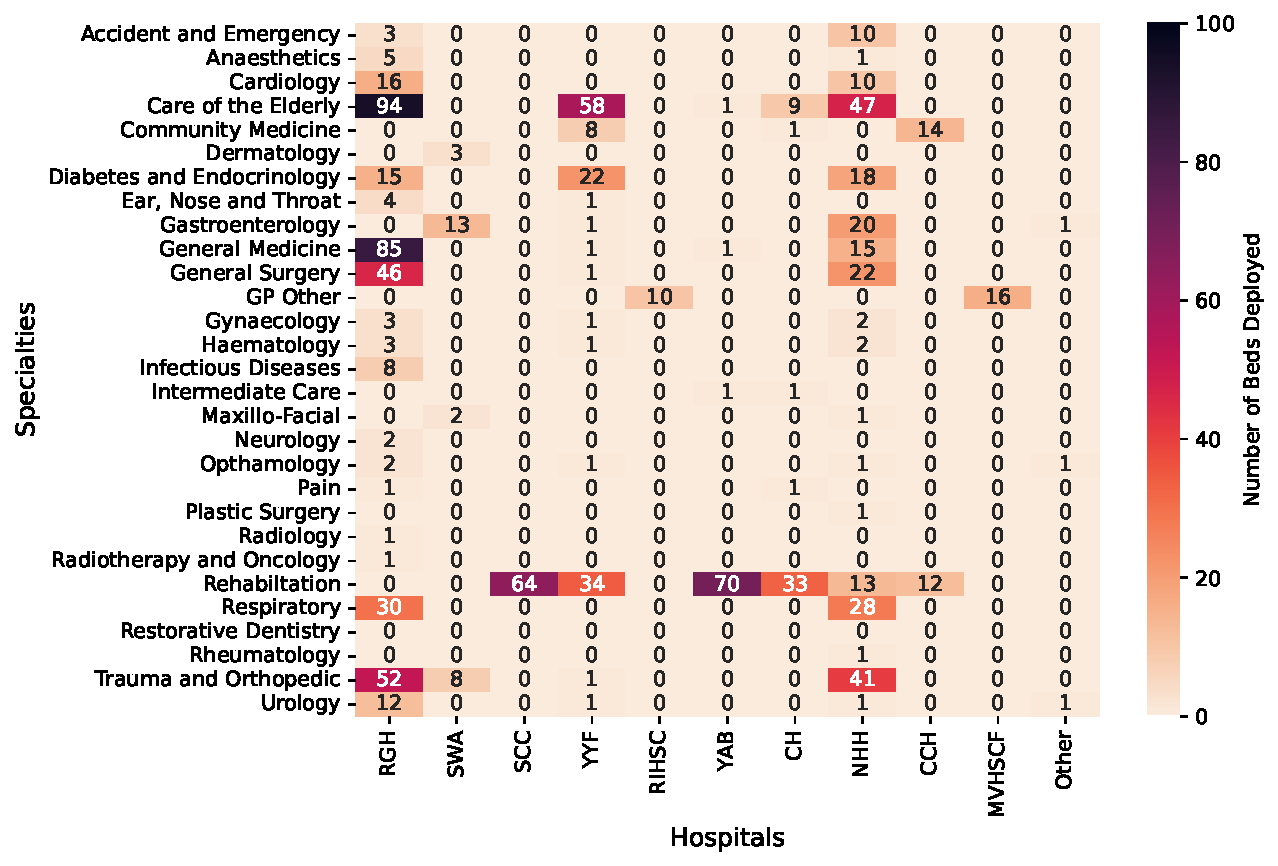
\includegraphics[scale=0.55]{Figures - Heatmaps/Fig15.pdf}
  \caption{Heatmap of bed locations for each specialty within each hospital for the deterministic model using the regression tree and specific LOS over three years' worth of data.}
    \label{fig:app10a}
\end{figure}
\begin{figure}[h!]
    \centering
    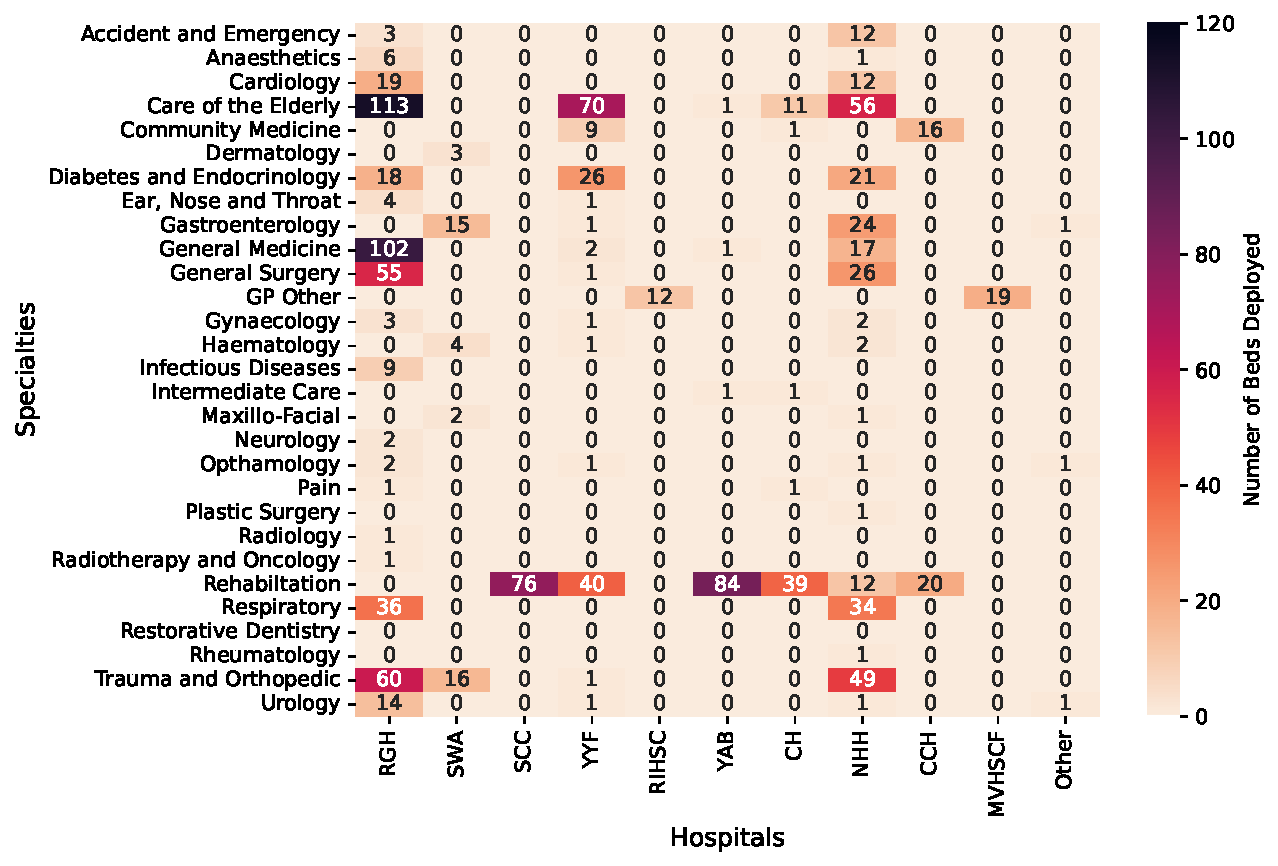
\includegraphics[scale=0.55]{Figures - Heatmaps/Fig16.pdf}
  \caption{Heatmap of bed locations for each specialty within each hospital for the two-stage stochastic model using the regression tree and specific LOS over three years' worth of data.}
    \label{fig:app10b}
\end{figure}

\begin{landscape}
    \begin{table}[h!]
    \centering\scalebox{0.8}{
    \begin{tabular}{lcccccccccccccccccc}\toprule
\multirow{2}{*}{\textbf{Specialty}}& \multicolumn{3}{c}{\textbf{Region 1}} & \multicolumn{3}{c}{\textbf{Region 2}}& \multicolumn{3}{c}{\textbf{Region 3}}\\\cmidrule(lr){2-4} \cmidrule(lr){5-7}\cmidrule(lr){8-10}
& \textbf{2017-2018} & \textbf{2018-2019} & \textbf{2019-2020} & \textbf{2017-2018} & \textbf{2018-2019} & \textbf{2019-2020} & \textbf{2017-2018} & \textbf{2018-2019} & \textbf{2019-2020} \\\midrule
Accident \& Emergency&	2.2932&	2.2000&	1.8579&	0.0000&	0.0000&	0.0000&	0.0000&	0.0000&	0.0000\\
Anaesthetics	&4.4932&	4.4712&	4.8033&	0.0000&	0.0000&	0.0000&	0.0000&	0.0000&	0.0000\\
Cardiology	&16.7918&	14.0630&	15.7240&	0.0000&	0.0000&	0.0000&	0.0000&	0.0000&	0.0000\\
Care of the Elderly&	76.4575&	88.0658&	117.3443&	55.8247&	58.4877&	58.8907&	0.0000&	0.4000&	1.8689\\
Community Medicine&	0.0000&	0.0000&	0.0000&	7.1671&	6.1014&	7.7514&	0.0000&	0.0000&	0.0000\\
Dermatology	&2.6877&	1.9918&	2.0984&	0.0000&	0.0000&	0.0000&	0.0000&	0.0000&	0.0000\\
Diabetes and Endocrinology&	16.5863&	11.4356&	15.3224&	24.7041&	19.8055&	19.2186&	0.0000&	0.0000&	0.0000\\
Ear Nose \& Throat&	2.9616&	3.6192&	2.7514&	0.0027&	0.0000&	0.0000&	0.0000&	0.0000&	0.0000\\
Gastroenterology	&11.4438&	9.8219&	15.6612&	0.1260&	0.0219&	0.1475&	0.0000&	0.0000&	0.0000\\
General Medicine&	105.6712&	96.0603&	51.8142&	0.2877&	1.1479&	1.5082&	0.0000&	0.0000&	0.0355\\
General Surgery&	47.9068&	45.3479&	43.3087&	0.2000&	0.2301&	0.2650&	0.0000&	0.0000&	0.0000\\
GP Other&	0.0000&	0.0000&	0.0000&	9.6795&	10.1151&	9.8224&	0.0000&	0.0000&	0.0000\\
Gynaecology	&2.4301&	1.7233&	1.8607&	0.0795&	0.0740&	0.0628&	0.0000&	0.0000&	0.0000\\
Haematology	&3.1096&	2.4384&	2.7896&	0.0000&	0.0000&	0.0792&	0.0000&	0.0000&	0.0000\\
Infectious Diseases&	8.0767&	6.3918&	6.8907&	0.0000&	0.0000&	0.0000&	0.0000&	0.0000&	0.0000\\
Intermediate Care&	0.0000&	0.0000&	0.0000&	0.0000&	0.0000&	0.0000&	0.0000&	0.0082&	1.0246\\
Maxillo-Facial&	1.1068&	0.9178&	1.1393&	0.0000&	0.0000&	0.0000&	0.0000&	0.0000&	0.0000\\
Neurology	&1.4301&	1.5534&	1.7022&	0.0000&	0.0000&	0.0000&	0.0000&	0.0000&	0.0000\\
Ophthalmology	&1.4712&	1.2685&	1.3716&	0.0000&	0.0000&	0.0082&	0.0000&	0.0000&	0.0000\\
Pain	&0.0000&	0.0000&	0.0055&	0.0000&	0.0000&	0.0000&	0.0000&	0.0000&	0.0000\\
Plastic Surgery&	0.0000&	0.0000&	0.0000&	0.0000&	0.0000&	0.0000&	0.0000&	0.0000&	0.0000\\
Radiology	&0.0055&	0.0164&	0.0082&	0.0000&	0.0000&	0.0000&	0.0000&	0.0000&	0.0000\\
Radiotherapy and Oncology&	0.0000&	0.0000&	0.6721&	0.0000&	0.0000&	0.0000&	0.0000&	0.0000&	0.0000\\
Rehabilitation	&64.7671&	63.1151&	61.1749&	34.9123&	34.8384&	29.5355&	69.9671&	65.3863&	73.0956\\
Respiratory	&29.8658&	30.4137&	28.1393&	0.0000&	0.0000&	0.0000&	0.0000&	0.0000&	0.0000\\
Restorative Dentistry&	0.0000&	0.0000&	0.0000&	0.0000&	0.0000&	0.0000&	0.0000&	0.0000&	0.0000\\
Rheumatology	&0.0000&	0.0000&	0.0000&	0.0000&	0.0000&	0.0000&	0.0000&	0.0000&	0.0000\\
Trauma \& Orthopaedic&	56.0082&	60.6164&	60.9126&	0.3808&	0.2712&	0.2350&	0.0000&	0.0000&	0.0000\\
Urology	&10.3671&	12.5726&	11.0383&	0.0027&	0.0055&	0.0027&	0.0000&	0.0000&	0.0000\\

\bottomrule
\end{tabular}  } 
\caption{The daily bed demands for each specialty for regions one, two and three within ABUHB for three individual years’ worth of patient admissions, using the regression tree and the year specific LOS.}
%\caption{Regions One, Two and Three Daily Demands for Three Individual Years of ABUHB Patient Admissions to Four Decimal Places - Regression Tree and Year Specific LOS}
    \label{apptab:LinkedDemands5a}
\end{table}

    \begin{table}[h!]
    \centering\scalebox{0.8}{
    \begin{tabular}{lcccccccccccccccccc}\toprule
\multirow{2}{*}{\textbf{Specialty}}& \multicolumn{3}{c}{\textbf{Region 4}} & \multicolumn{3}{c}{\textbf{Region 5}}& \multicolumn{3}{c}{\textbf{Region 6}}\\\cmidrule(lr){2-4} \cmidrule(lr){5-7}\cmidrule(lr){8-10}
& \textbf{2017-2018} & \textbf{2018-2019} & \textbf{2019-2020} & \textbf{2017-2018} & \textbf{2018-2019} & \textbf{2019-2020} & \textbf{2017-2018} & \textbf{2018-2019} & \textbf{2019-2020} \\\midrule
Accident \& Emergency&	0.0000&	0.0000&	0.0000&	8.5452&	10.0630&	8.9208&	0.0000&	0.0000&	0.0000\\
Anaesthetics&	0.0000&	0.0000&	0.0000&	0.4247&	0.7753&	1.1148&	0.0000&	0.0000&	0.0000\\
Cardiology&	0.0000&	0.0000&	0.0000&	10.6603&	10.2137&	8.5000&	0.0000&	0.0000&	0.0000\\
Care of the Elderly&	12.4192&	6.5233&	7.4180&	53.7178&	44.1726&	41.4426&	0.0000&	0.0000&	0.0000\\
Community Medicine&	0.3671&	0.1397&	0.4344&	16.7151&	14.0466&	8.2923&	0.0000&	0.0000&	0.0000\\
Dermatology&	0.0000&	0.0000&	0.0000&	0.0000&	0.0000&	0.0000&	0.0000&	0.0000&	0.0000\\
Diabetes and Endocrinology&	0.0000&	0.0000&	0.0000&	17.8575&	18.4000&	15.4344&	0.0000&	0.0000&	0.0000\\
Ear Nose \& Throat&	0.0000&	0.0000&	0.0000&	0.0000&	0.0000&	0.0000&	0.0000&	0.0000&	0.0000\\
Gastroenterology&	0.0000&	0.0000&	0.0000&	18.0164&	21.3781&	19.9344&	0.0000&	0.0000&	0.0027\\
General Medicine&	0.0000&	0.0000&	0.0000&	11.9644&	11.7342&	18.5929&	0.0000&	0.0000&	0.0000\\
General Surgery&	0.0000&	0.0000&	0.0000&	21.1041&	22.6219&	20.1803&	0.0000&	0.0000&	0.0000\\
GP Other&	0.0000&	0.0000&	0.0000&	14.7781&	13.8740&	17.2732&	0.0000&	0.0000&	0.0000\\
Gynaecology&	0.0000&	0.0000&	0.0000&	1.1753&	1.4438&	0.6120&	0.0000&	0.0000&	0.0000\\
Haematology&	0.0000&	0.0000&	0.0000&	1.2932&	1.0438&	1.0628&	0.0000&	0.0000&	0.0000\\
Infectious Diseases&	0.0000&	0.0000&	0.0000&	0.0000&	0.0000&	0.0000&	0.0000&	0.0000&	0.0000\\
Intermediate Care&	0.0000&	0.6000&	0.3716&	0.0000&	0.0000&	0.0000&	0.0000&	0.0000&	0.0000\\
Maxillo-Facial&	0.0000&	0.0000&	0.0000&	0.0000&	0.0000&	0.0082&	0.0000&	0.0000&	0.0000\\
Neurology&	0.0000&	0.0000&	0.0000&	0.0000&	0.0000&	0.0000&	0.0000&	0.0000&	0.0000\\
Ophthalmology&	0.0000&	0.0000&	0.0000&	0.0000&	0.0000&	0.0027&	0.0000&	0.0055&	0.0055\\
Pain&	0.0055&	0.0000&	0.0000&	0.0000&	0.0000&	0.0000&	0.0000&	0.0000&	0.0000\\
Plastic Surgery&	0.0000&	0.0000&	0.0000&	0.0000&	0.0000&	0.0410&	0.0000&	0.0000&	0.0000\\
Radiology&	0.0000&	0.0000&	0.0000&	0.0000&	0.0000&	0.0000&	0.0000&	0.0000&	0.0000\\
Radiotherapy and Oncology&	0.0000&	0.0000&	0.0000&	0.0000&	0.0000&	0.0000&	0.0000&	0.0000&	0.0000\\
Rehabilitation&	29.6877&	33.0521&	33.5792&	18.3918&	25.3288&	29.9262&	0.0000&	0.0000&	0.0000\\
Respiratory&	0.0000&	0.0000&	0.0000&	30.6411&	29.4301&	23.1284&	0.0000&	0.0000&	0.0000\\
Restorative Dentistry&	0.0000&	0.0000&	0.0000&	0.0000&	0.0000&	0.0000&	0.0000&	0.0000&	0.0000\\
Rheumatology&	0.0000&	0.0000&	0.0000&	0.0000&	0.0384&	0.0000&	0.0000&	0.0000&	0.0000\\
Trauma \& Orthopaedic&	0.0000&	0.0000&	0.0000&	41.8192&	40.3178&	39.9617&	0.0000&	0.0000&	0.0000\\
Urology&	0.0000&	0.0000&	0.0000&	0.0110&	0.0192&	0.0464&	0.0384&	0.0384&	0.0437\\

\bottomrule
\end{tabular}} 
\caption{The daily bed demands for each specialty for regions four, five and six within ABUHB for three individual years’ worth of patient admissions, using the regression tree and the year specific LOS.}
    \label{apptab:LinkedDemands5b}
\end{table}
\end{landscape}
\begin{landscape}
    
\begin{figure}[h!]
\centering
\begin{minipage}{0.4\linewidth}
  \centering
  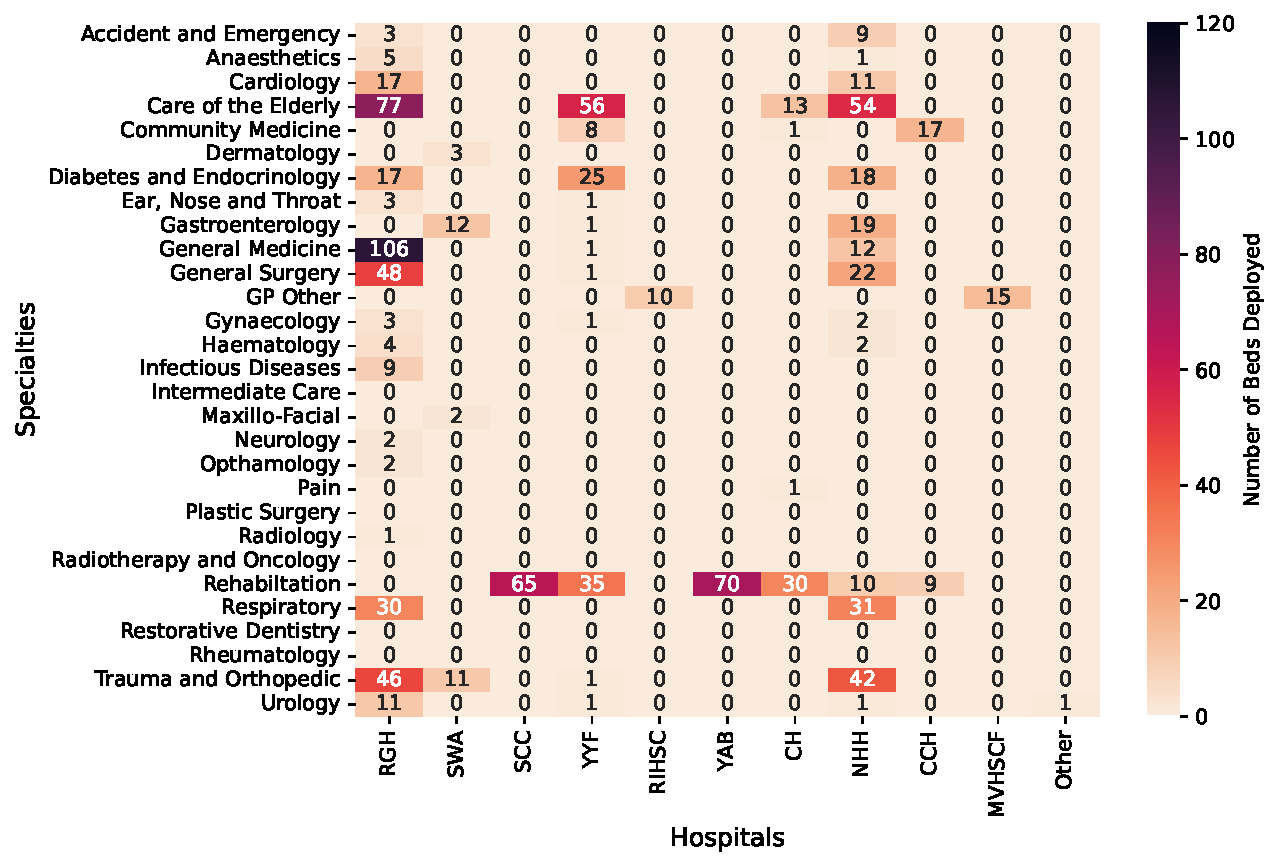
\includegraphics[scale=0.4]{Figures - Heatmaps/Fig17.pdf}
  \captionsetup{font={scriptsize}}
  \captionof{figure}{{Heatmap of bed locations for each specialty within each\\ hospital for the deterministic model using the regression tree and \\specific LOS for 2017-2018.}}
  \label{fig:app11a}
\end{minipage}%
\begin{minipage}{0.4\linewidth}
  \centering
  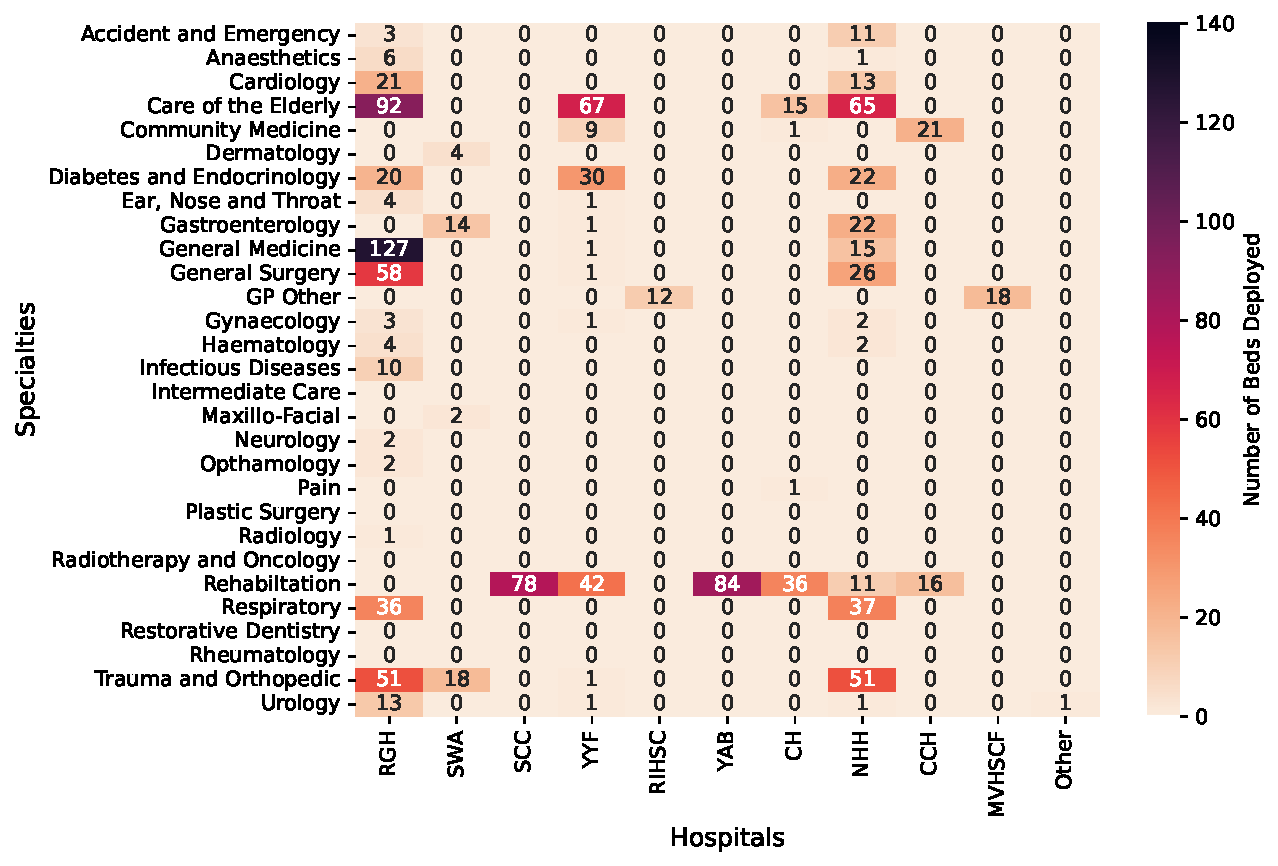
\includegraphics[scale=0.4]{Figures - Heatmaps/Fig18.pdf}  \captionsetup{font={scriptsize}}
  \captionof{figure}{Heatmap of bed locations for each specialty within each\\ hospital for the two-stage stochastic model using the regression tree and \\specific LOS for 2017-2018.}
  \label{fig:app11b}
\end{minipage}
\end{figure}

\begin{figure}[h!]
\centering
\begin{minipage}{0.4\linewidth}
  \centering
  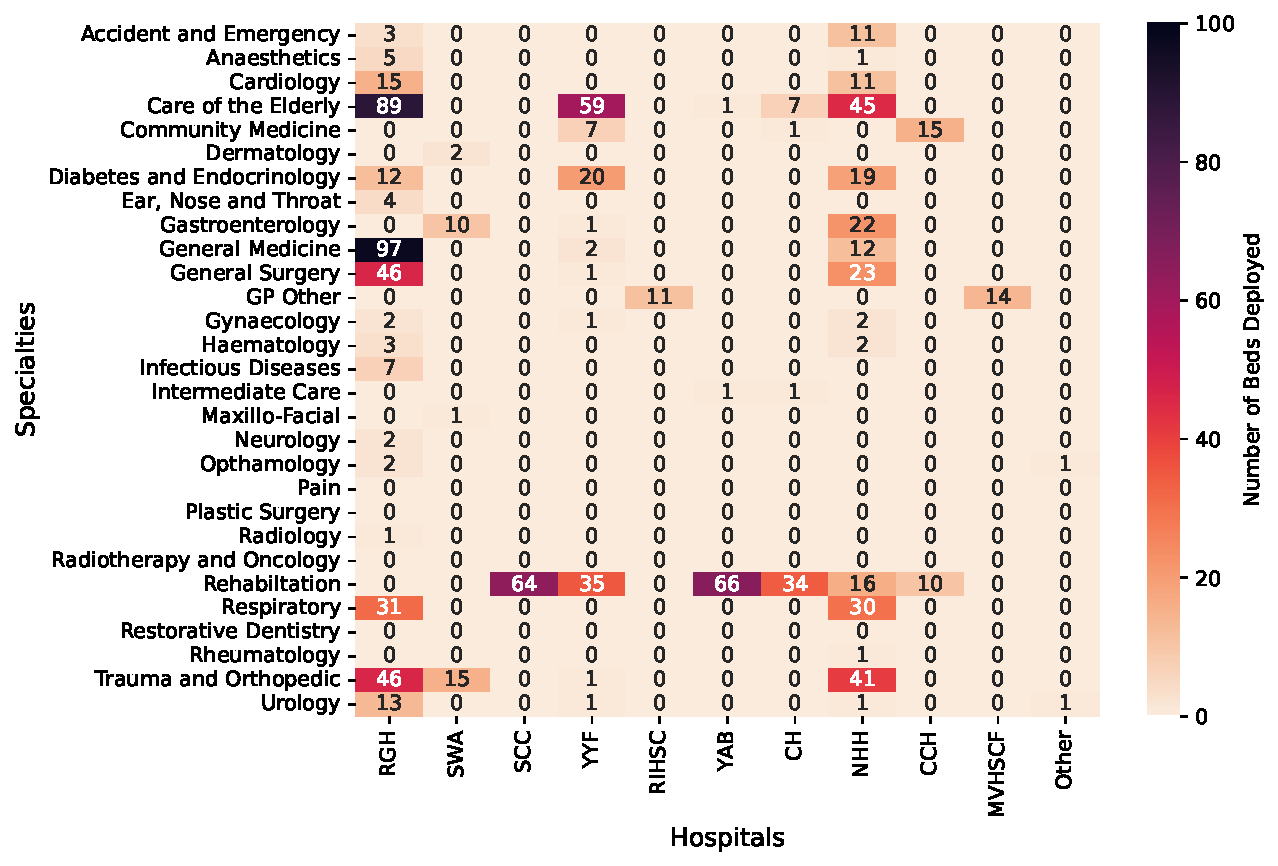
\includegraphics[scale=0.4]{Figures - Heatmaps/Fig19.pdf}
\captionsetup{font={scriptsize}}
  \captionof{figure}{{Heatmap of bed locations for each specialty within each\\ hospital for the deterministic model using the regression tree and \\specific LOS for 2018-2019.}}
  \label{fig:app12a}
\end{minipage}%
\begin{minipage}{0.4\linewidth}
  \centering
  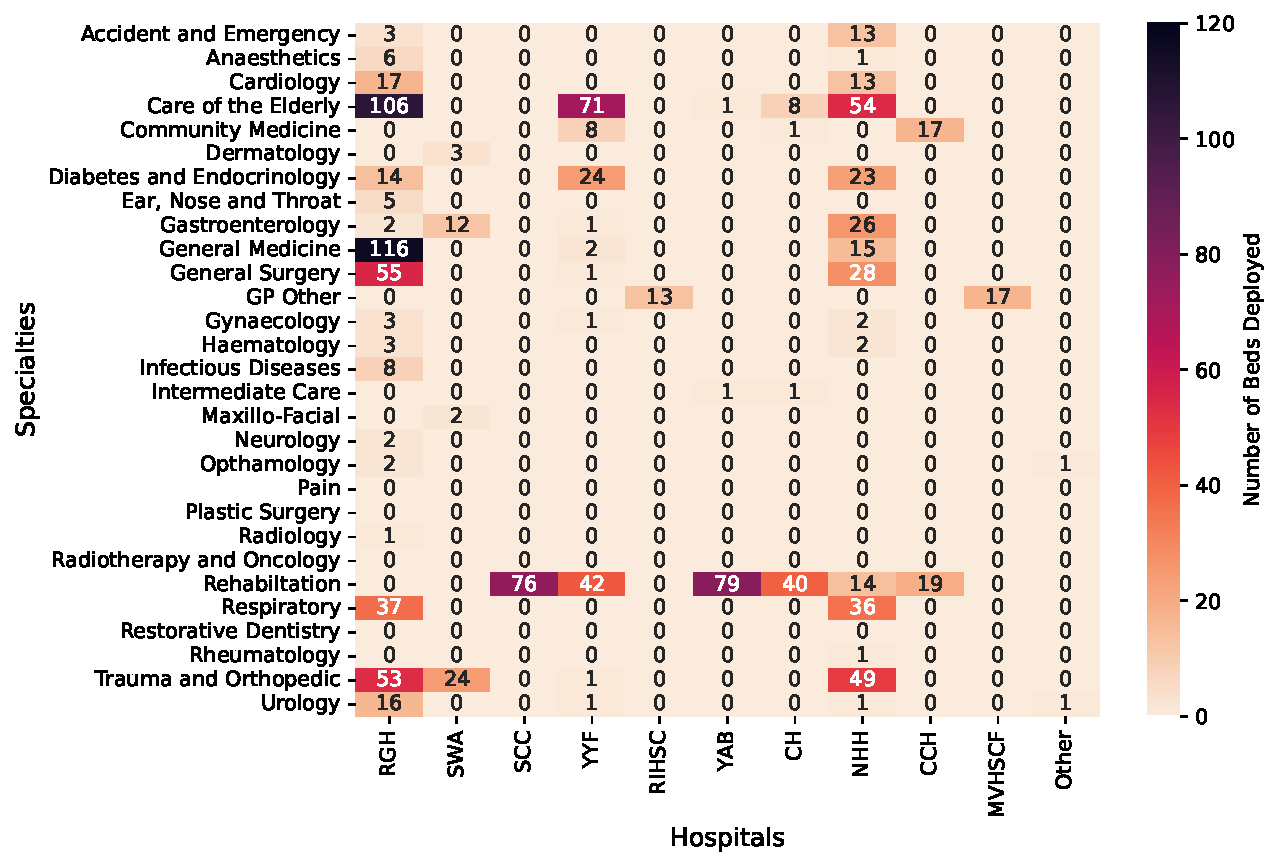
\includegraphics[scale=0.4]{Figures - Heatmaps/Fig20.pdf}
  \captionsetup{font={scriptsize}}
  \captionof{figure}{{Heatmap of bed locations for each specialty within each\\ hospital for the two-stage stochastic model using the regression tree and \\specific LOS for 2018-2019.}}
  \label{fig:app12b}
\end{minipage}
\end{figure}

\begin{figure}[h!]
\centering
\begin{minipage}{0.4\linewidth}
  \centering
  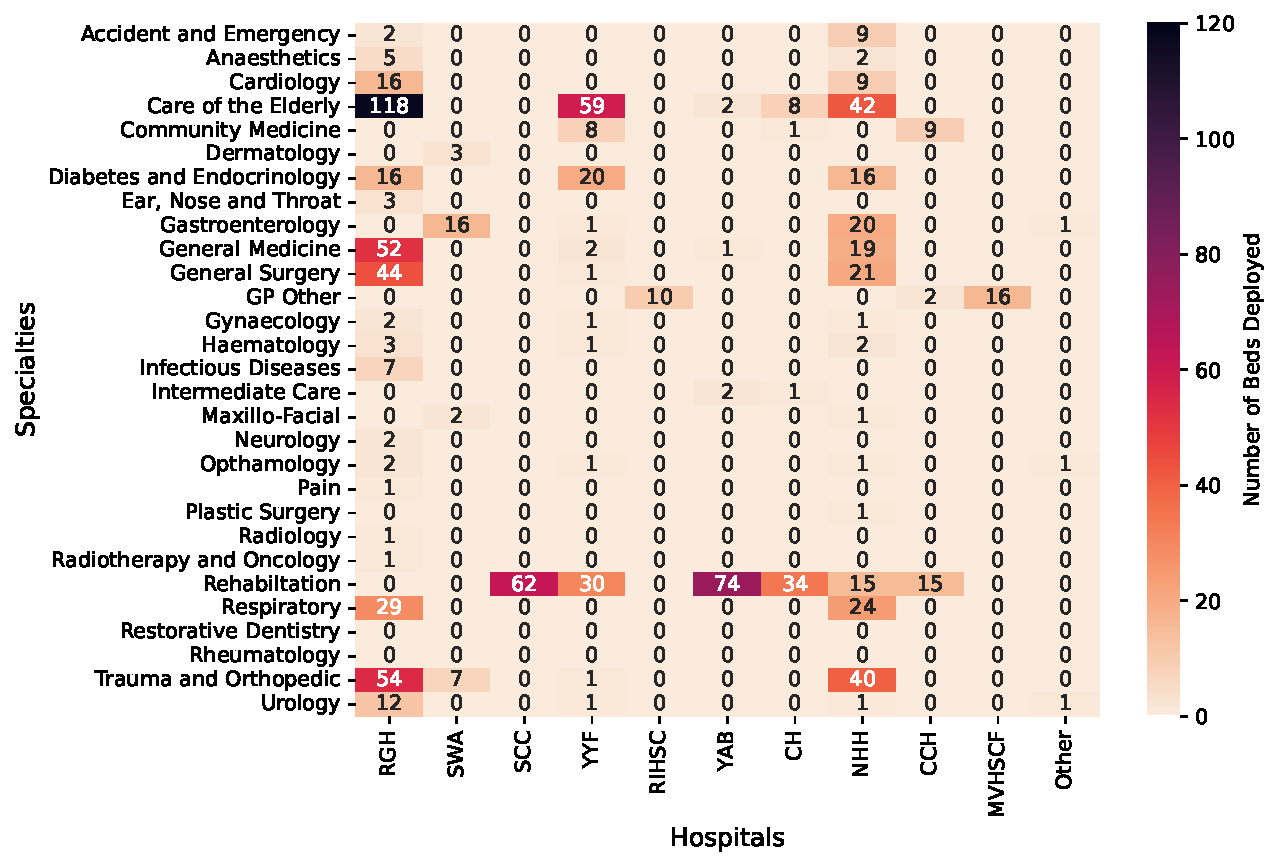
\includegraphics[scale=0.4]{Figures - Heatmaps/Fig21.pdf}
\captionsetup{font={scriptsize}}
  \captionof{figure}{{Heatmap of bed locations for each specialty within each\\ hospital for the deterministic model using the regression tree and \\specific LOS for 2019-2020.}}
  \label{fig:app13a}
\end{minipage}%
\begin{minipage}{0.4\linewidth}
  \centering
  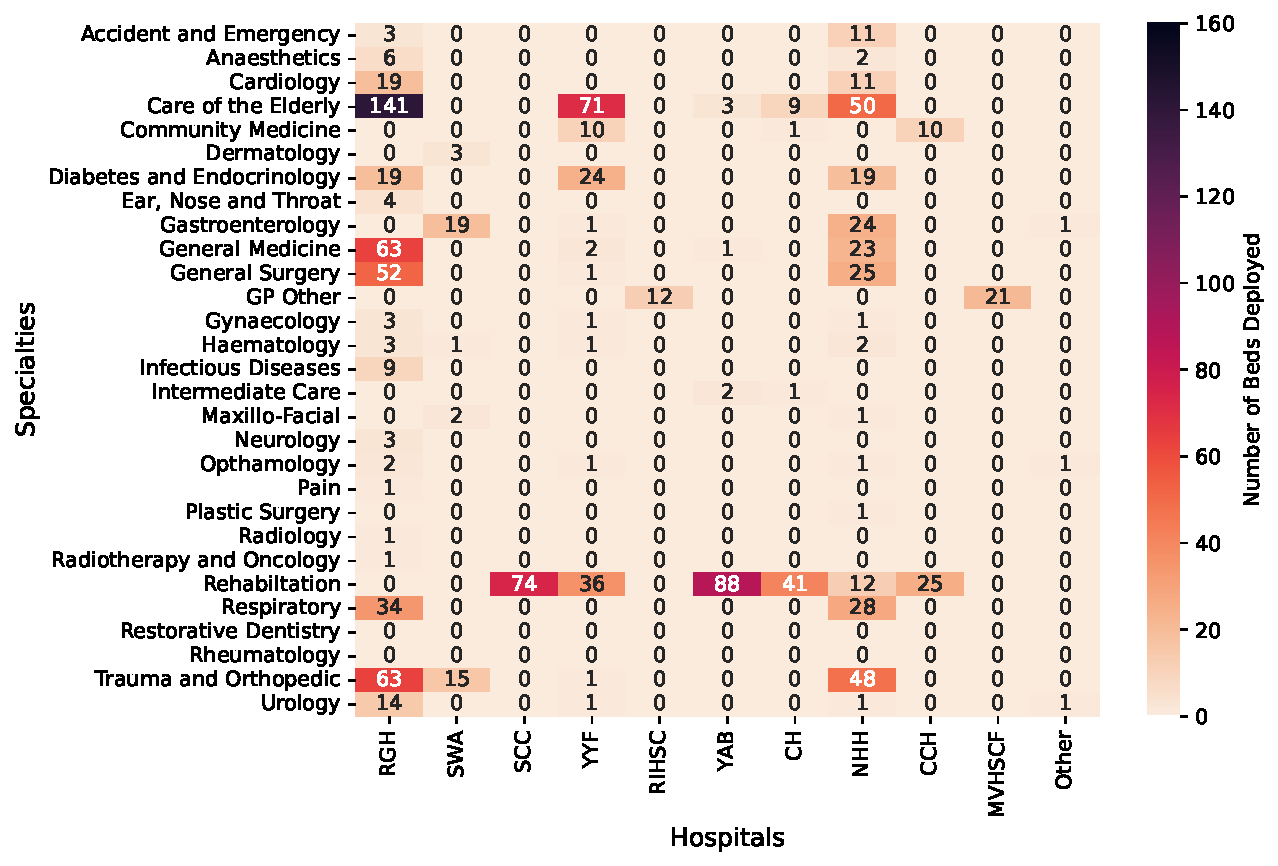
\includegraphics[scale=0.4]{Figures - Heatmaps/Fig22.pdf}
  \captionsetup{font={scriptsize}}
  \captionof{figure}{{Heatmap of bed locations for each specialty within each\\ hospital for the two-stage stochastic model using the regression tree and \\specific LOS for 2019-2020.}}
  \label{fig:app13b}
\end{minipage}
\end{figure}
\end{landscape}

\section{Classification Trees - Average LOS}

\begin{table}[h!]
    \centering\scalebox{0.78}{
    \begin{tabular}{ccccccc} \toprule
\textbf{Specialty} &	\textbf{Region 1}	&\textbf{Region 2}&	\textbf{Region 3}&	\textbf{Region 4}	&\textbf{Region 5}&	\textbf{Region 6} \\\midrule
Accident \& Emergency&	2.9437	&0.0000&	0.0000&	0.0000&	8.3492&	0.0000\\
Anaesthetics&	4.1522&	0.0000&	0.0000&	0.0000&	0.6332&	0.0000\\
Cardiology&	24.9347&	0.0000&	0.0000&	0.0000&	16.8229&	0.0001\\
Care of the Elderly&	119.0511&	46.6365&	0.5724&	3.8356&	58.7402&	0.0000\\
Community Medicine&	0.0000&	3.1172&	0.0000&	0.1218&	4.6880&	0.0000\\
Dermatology&	1.6374&	0.3027&	0.0000&	0.0000&	0.0000&	0.0000\\
Diabetes and Endocrinology&	18.8983	&17.7172&	0.0000&	0.0000&	24.1221&	0.0000\\
Ear Nose \& Throat&	6.9407&	0.0178&	0.0000&	0.0000&	0.0000&	0.0000\\
Gastroenterology&	15.9809&	0.6828&	0.0000&	0.0000&	27.8963&	0.0307\\
General Medicine&	83.8888&	0.4873&	0.0077&	0.0000&	15.2006&	0.0000\\
General Surgery&	64.0241&	0.3538&	0.0000&	0.0000&	33.8609&	0.0025\\
GP Other&	0.0000&	3.3973&	0.0000&	0.0000&	5.1629&	0.0000\\
Gynaecology&	2.8824&	0.2171&	0.0000&	0.0000&	1.4492&	0.0008\\
Haematology&	5.4136&	0.0635&	0.0000&	0.0000&	2.1941&	0.0001\\
Infectious Diseases&	8.1705&	0.0000&	0.0000&	0.0000&	0.0000&	0.0000\\
Intermediate Care&	0.0000&	0.0000&	0.2922&	0.3288&	0.0000&	0.0000\\
Maxillo-Facial&	1.2233	&0.0000&	0.0000&	0.0000&	0.0288&	0.0000\\
Neurology&	3.6535&	0.0000&	0.0000&	0.0000&	0.0000&	0.0000\\
Ophthalmology&	2.4715&	0.0122&	0.0000&	0.0000&	0.1323&	0.2449\\
Pain&	0.0335&	0.0033&	0.0000&	0.0045&	0.0136&	0.0000\\
Plastic Surgery&	0.0000&	0.0000&	0.0000&	0.0000&	0.0146&	0.0001\\
Radiology&	0.0262&	0.0000&	0.0000&	0.0000&	0.0135&	0.0000\\
Radiotherapy and Oncology&	0.0026	&0.0000&	0.0000&	0.0000&	0.0000&	0.0000\\
Rehabilitation&	26.2528&	13.1021&	38.7217&	14.1127&	10.8981&	0.0000\\
Respiratory&	39.6264&	0.0000&	0.0000&	0.0000&	42.5619&	0.0000\\
Restorative Dentistry&	0.0002&	0.0000&	0.0000&	0.0000&	0.0000&	0.0000\\
Rheumatology&	0.0001&	0.0487&	0.0000&	0.0000&	0.0122&	0.0000\\
Trauma \& Orthopaedic&	64.6427	&0.2885&	0.0000&	0.0000&	44.6021&	0.0000\\
Urology&	22.2711&	0.0411&	0.0000&	0.0000&	0.1389&	0.0043\\
\bottomrule


    \end{tabular}}
    \caption{The daily bed demands for each specialty grouped by regions within ABUHB for three years’ worth of patient admissions, using the classification tree and average LOS.}
    %\caption{Linked Predictive and Prescriptive Demands - Classification Tree and Average LOS - Three Years' Worth of Data}
    \label{apptab:LinkedDemands6}
\end{table}


\begin{figure}[h!]
    \centering
    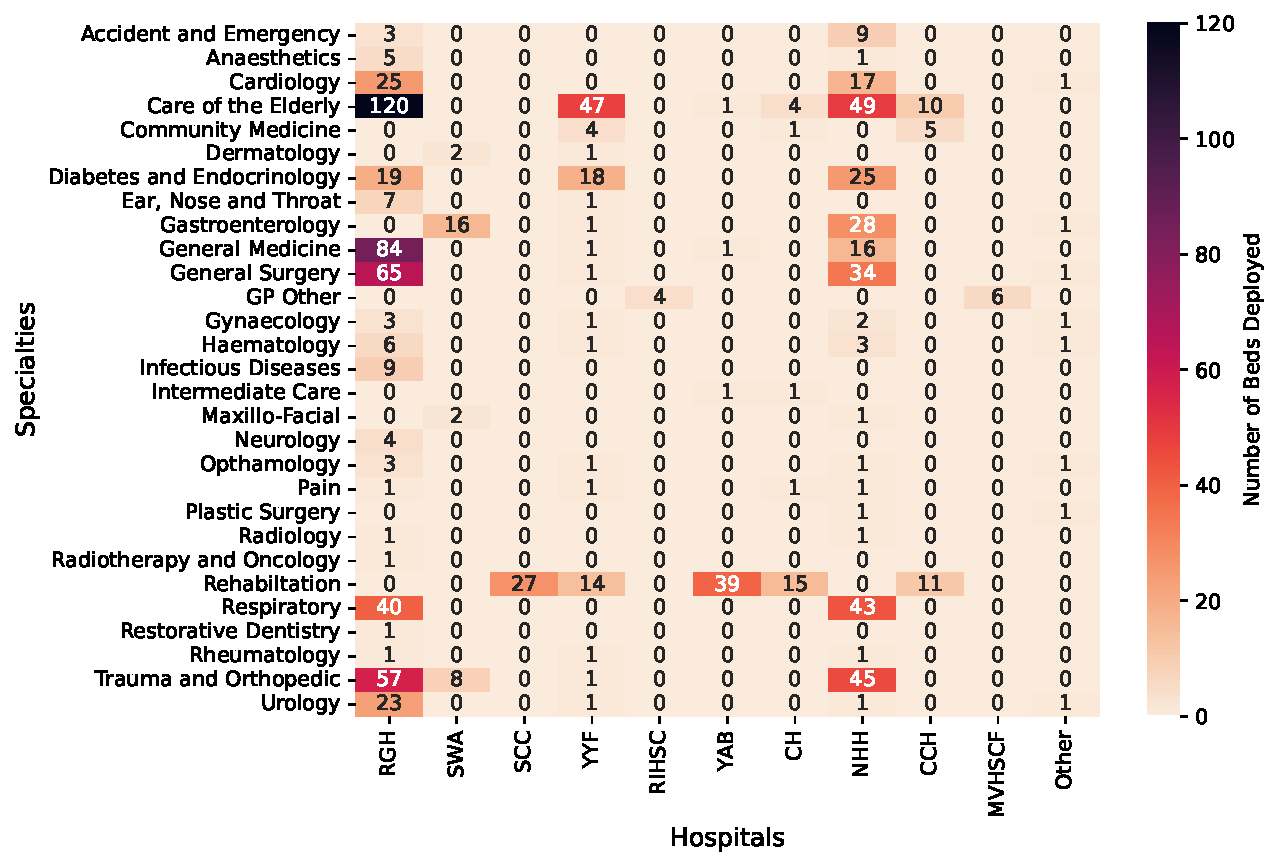
\includegraphics[scale=0.55]{Figures - Heatmaps/Fig23.pdf}
\caption{Heatmap of bed locations for each specialty within each hospital for the deterministic model using the classification tree and average LOS over three years' worth of data.}
    \label{fig:app14a}
\end{figure}
\begin{figure}[h!]
    \centering
    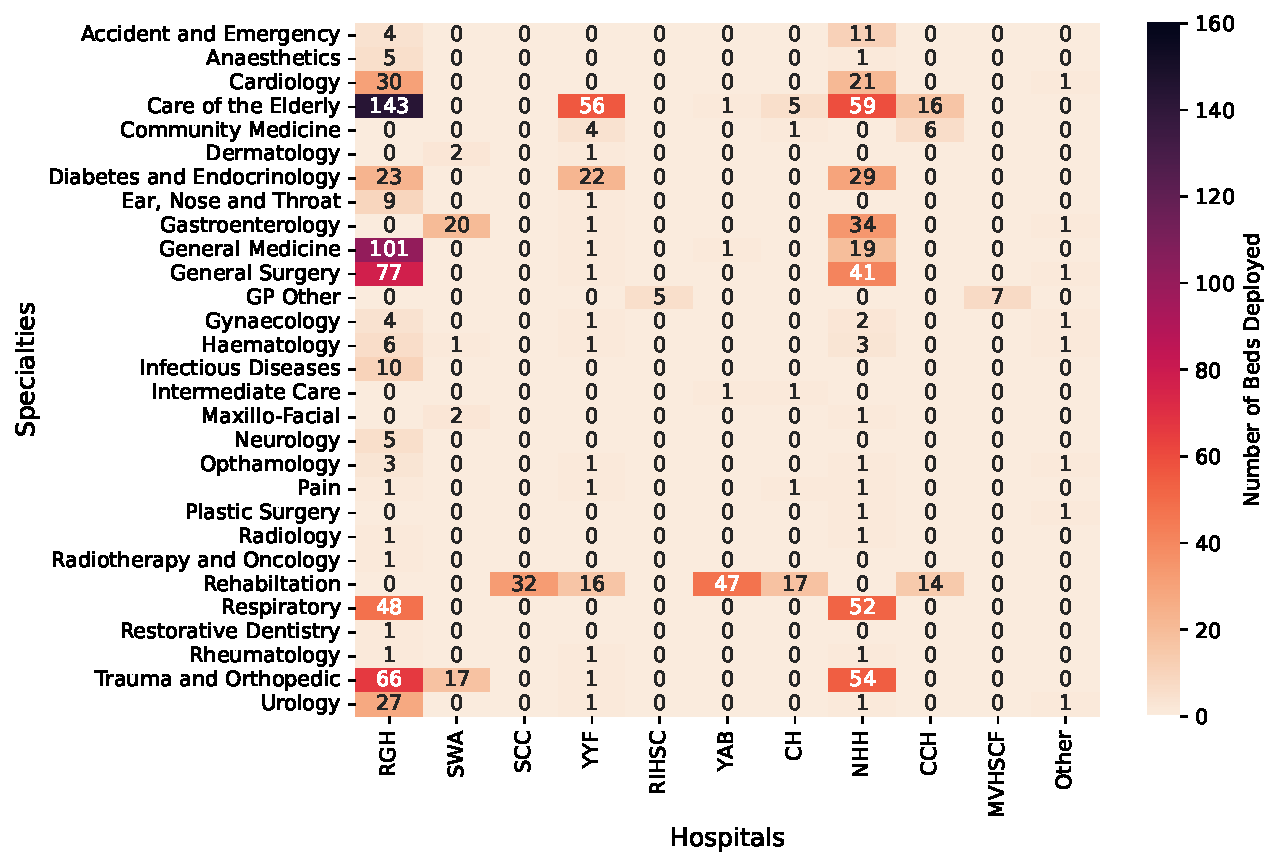
\includegraphics[scale=0.55]{Figures - Heatmaps/Fig24.pdf}
    \caption{Heatmap of bed locations for each specialty within each hospital for the two-stage stochastic model using the classification tree and average LOS over three years' worth of data.}
    \label{fig:app14b}
\end{figure}

\begin{landscape}

   \begin{table}[h!]
    \centering\scalebox{0.8}{
    \begin{tabular}{lcccccccccccccccccc}\toprule
\multirow{2}{*}{\textbf{Specialty}}& \multicolumn{3}{c}{\textbf{Region 1}} & \multicolumn{3}{c}{\textbf{Region 2}}& \multicolumn{3}{c}{\textbf{Region 3}}\\\cmidrule(lr){2-4} \cmidrule(lr){5-7}\cmidrule(lr){8-10}
& \textbf{2017-2018} & \textbf{2018-2019} & \textbf{2019-2020} & \textbf{2017-2018} & \textbf{2018-2019} & \textbf{2019-2020} & \textbf{2017-2018} & \textbf{2018-2019} & \textbf{2019-2020} \\\midrule
Accident \& Emergency&	3.2363&	3.1680&	2.4283&	0.0000&	0.0000&	0.0000&	0.0000&	0.0000&	0.0000\\
Anaesthetics&	4.4607&	3.7660&	4.2297&	0.0000&	0.0000&	0.0000&	0.0000&	0.0000&	0.0000\\
Cardiology&	24.2501&	22.6507&	27.8952&	0.0000&	0.0000&	0.0000&	0.0000&	0.0000&	0.0000\\
Care of the Elderly&	99.2695&	117.1490&	140.6756&	45.0459&	48.8485&	46.0167&	0.0000&	0.1463&	1.5683\\
Community Medicine&	0.0000&	0.0000&	0.0000&	3.1079&	2.9616&	3.2817&	0.0000&	0.0000&	0.0000\\
Dermatology&	1.5668&	1.8460&	1.4996&	0.2500&	0.3673&	0.2910&	0.0000&	0.0000&	0.0000\\
Diabetes and Endocrinology&	20.5858&	15.1737&	20.9300&	19.0863&	17.3310&	16.7370&	0.0000&	0.0000&	0.0000\\
Ear Nose \& Throat&	7.4638&	6.8977&	6.4620&	0.0344&	0.0115&	0.0076&	0.0000&	0.0000&	0.0000\\
Gastroenterology&	15.5449&	12.0964&	20.2896&	0.7179&	0.6021&	0.7282&	0.0000&	0.0000&	0.0000\\
General Medicine&	97.5751&	94.9051&	59.2536&	0.2090&	0.4413&	0.8107&	0.0000&	0.0000&	0.0232\\
General Surgery&	63.3663&	66.2451&	62.4650&	0.2488&	0.3001&	0.5120&	0.0000&	0.0000&	0.0000\\
GP Other&	0.0000&	0.0000&	0.0000&	3.0713&	3.5466&	3.5734&	0.0000&	0.0000&	0.0000\\
Gynaecology&	3.0095&	2.4954&	3.1416&	0.3757&	0.1601&	0.1158&	0.0000&	0.0000&	0.0000\\
Haematology&	5.7301&	4.5135&	5.9957&	0.0000&	0.0000&	0.1902&	0.0000&	0.0000&	0.0000\\
Infectious Diseases&	9.3236&	7.5686&	7.6208&	0.0000&	0.0000&	0.0000&	0.0000&	0.0000&	0.0000\\
Intermediate Care&	0.0000&	0.0000&	0.0000&	0.0000&	0.0000&	0.0000&	0.0000&	0.0366&	0.8387\\
Maxillo-Facial&	1.3817&	1.3665&	0.9226&	0.0000&	0.0000&	0.0000&	0.0000&	0.0000&	0.0000\\
Neurology&	4.2779&	3.2917&	3.3918&	0.0000&	0.0000&	0.0000&	0.0000&	0.0000&	0.0000\\
Ophthalmology&	2.4465&	2.5135&	2.4547&	0.0000&	0.0000&	0.0365&	0.0000&	0.0000&	0.0000\\
Pain&	0.0338&	0.0388&	0.0281&	0.0000&	0.0070&	0.0030&	0.0000&	0.0000&	0.0000\\
Plastic Surgery&	0.0000&	0.0000&	0.0000&	0.0000&	0.0000&	0.0000&	0.0000&	0.0000&	0.0000\\
Radiology&	0.0020&	0.0379&	0.0388&	0.0000&	0.0000&	0.0000&	0.0000&	0.0000&	0.0000\\
Radiotherapy and Oncology&	0.0042&	0.0025&	0.0010&	0.0000&	0.0000&	0.0000&	0.0000&	0.0000&	0.0000\\
Rehabilitation&	28.3000&	24.9361&	25.5243&	13.5650&	13.8940&	11.8506&	33.5651&	36.2707&	46.3084\\
Respiratory&	42.2210&	39.5059&	38.5387&	0.0000&	0.0000&	0.0000&	0.0000&	0.0000&	0.0000\\
Restorative Dentistry&	0.0003&	0.0000&	0.0003&	0.0000&	0.0000&	0.0000&	0.0000&	0.0000&	0.0000\\
Rheumatology&	0.0000&	0.0000&	0.0003&	0.0000&	0.1463&	0.0000&	0.0000&	0.0000&	0.0000\\
Trauma \& Orthopaedic&	59.6046&	71.7496&	62.5797&	0.2491&	0.3731&	0.2435&	0.0000&	0.0000&	0.0000\\
Urology&	20.1980&	23.1760&	23.4361&	0.0136&	0.0981&	0.0116&	0.0000&	0.0000&	0.0000\\
\bottomrule

    \end{tabular}  } 
    \caption{The daily bed demands for each specialty for regions one, two and three within ABUHB for three individual years’ worth of patient admissions, using the classification tree and the node average LOS.}
%\caption{Regions One, Two and Three Daily Demands for Three Individual Years of ABUHB Patient Admissions to Four Decimal Places - Classification Tree and Average Node LOS}
    \label{apptab:LinkedDemands7a}
\end{table}


   \begin{table}[h!]
    \centering\scalebox{0.8}{
    \begin{tabular}{lcccccccccccccccccc}\toprule
\multirow{2}{*}{\textbf{Specialty}}& \multicolumn{3}{c}{\textbf{Region 4}} & \multicolumn{3}{c}{\textbf{Region 5}}& \multicolumn{3}{c}{\textbf{Region 6}}\\\cmidrule(lr){2-4} \cmidrule(lr){5-7}\cmidrule(lr){8-10}
& \textbf{2017-2018} & \textbf{2018-2019} & \textbf{2019-2020} & \textbf{2017-2018} & \textbf{2018-2019} & \textbf{2019-2020} & \textbf{2017-2018} & \textbf{2018-2019} & \textbf{2019-2020} \\\midrule
Accident \& Emergency&	0.0000&	0.0000&	0.0000&	7.6680&	8.6804&	9.9681&	0.0000&	0.0000&	0.0000\\
Anaesthetics&	0.0000&	0.0000&	0.0000&	0.4638&	0.4268&	0.9722&	0.0000&	0.0000&	0.0000\\
Cardiology&	0.0000&	0.0000&	0.0000&	16.1539&	14.2806&	11.1400&	0.0000&	0.0000&	0.0011\\
Care of the Elderly&	12.5281&	6.5938&	6.8223&	52.3094&	45.1508&	41.2107&	0.0000&	0.0000&	0.0000\\
Community Medicine&	0.4234&	0.2117&	0.4222&	14.1831&	15.4549&	9.9576&	0.0000&	0.0000&	0.0000\\
Dermatology&	0.0000&	0.0000&	0.0000&	0.0000&	0.0000&	0.0000&	0.0000&	0.0000&	0.0000\\
Diabetes and Endocrinology&	0.0000&	0.0000&	0.0000&	16.6698&	17.8823&	15.3511&	0.0000&	0.0000&	0.0000\\
Ear Nose \& Throat&	0.0000&	0.0000&	0.0000&	0.0000&	0.0000&	0.0000&	0.0000&	0.0000&	0.0000\\
Gastroenterology&	0.0000&	0.0000&	0.0000&	18.7998&	21.9374&	19.9778&	0.3047&	0.0000&	0.0022\\
General Medicine&	0.0000&	0.0000&	0.0000&	13.9936&	14.0130&	20.9445&	0.0000&	0.0000&	0.0000\\
General Surgery&	0.0000&	0.0000&	0.0000&	20.4583&	21.6905&	21.4020&	0.0011&	0.0011&	0.0011\\
GP Other&	0.0000&	0.0000&	0.0000&	14.1544&	13.2848&	14.3738&	0.0000&	0.0000&	0.0000\\
Gynaecology&	0.0000&	0.0000&	0.0000&	0.9738&	0.9246&	0.6943&	0.0000&	0.0000&	0.0011\\
Haematology&	0.0000&	0.0000&	0.0000&	1.8249&	1.7582&	2.0842&	0.0011&	0.0000&	0.0000\\
Infectious Diseases&	0.0000&	0.0000&	0.0000&	0.0000&	0.0000&	0.0000&	0.0000&	0.0000&	0.0000\\
Intermediate Care&	0.0000&	0.3333&	0.3699&	0.0000&	0.0000&	0.0000&	0.0000&	0.0000&	0.0000\\
Maxillo-Facial&	0.0000&	0.0000&	0.0000&	0.1061&	0.0747&	0.0969&	0.0000&	0.0000&	0.0000\\
Neurology&	0.0000&	0.0000&	0.0000&	0.0000&	0.0000&	0.0000&	0.0000&	0.0000&	0.0000\\
Ophthalmology&	0.0000&	0.0000&	0.0000&	0.3948&	0.4613&	0.4636&	0.0000&	0.9640&	1.2960\\
Pain&	0.0166&	0.0110&	0.0176&	0.0519&	0.0442&	0.0396&	0.0000&	0.0000&	0.0000\\
Plastic Surgery&	0.0000&	0.0000&	0.0000&	0.0521&	0.0464&	0.0462&	0.0000&	0.0000&	0.0011\\
Radiology&	0.0000&	0.0000&	0.0000&	0.0091&	0.0011&	0.0225&	0.0000&	0.0000&	0.0000\\
Radiotherapy and Oncology&	0.0000&	0.0000&	0.0000&	0.0000&	0.0000&	0.0000&	0.0000&	0.0000&	0.0000\\
Rehabilitation&	29.5478&	33.4318&	35.5989&	10.7206&	16.2437&	23.0764&	0.0000&	0.0000&	0.0000\\
Respiratory&	0.0000&	0.0000&	0.0000&	32.7445&	29.8673&	25.8748&	0.0000&	0.0000&	0.0000\\
Restorative Dentistry&	0.0000&	0.0000&	0.0000&	0.0000&	0.0000&	0.0000&	0.0000&	0.0000&	0.0000\\
Rheumatology&	0.0000&	0.0000&	0.0000&	0.0000&	0.0215&	0.0000&	0.0000&	0.0000&	0.0000\\
Trauma \& Orthopaedic&	0.0000&	0.0000&	0.0000&	36.3659&	44.0053&	41.3888&	0.0000&	0.0000&	0.0000\\
Urology&	0.0000&	0.0000&	0.0000&	0.5179&	0.4967&	0.5494&	0.0210&	0.0169&	0.0226\\
\bottomrule


    \end{tabular}  } 
    \caption{The daily bed demands for each specialty for regions four, five and six within ABUHB for three individual years’ worth of patient admissions, using the classification tree and the node average LOS.}
    \label{apptab:LinkedDemands7b}
\end{table}
\end{landscape}

\begin{landscape}
    
\begin{figure}[h!]
\centering
\begin{minipage}{0.4\linewidth}
  \centering
  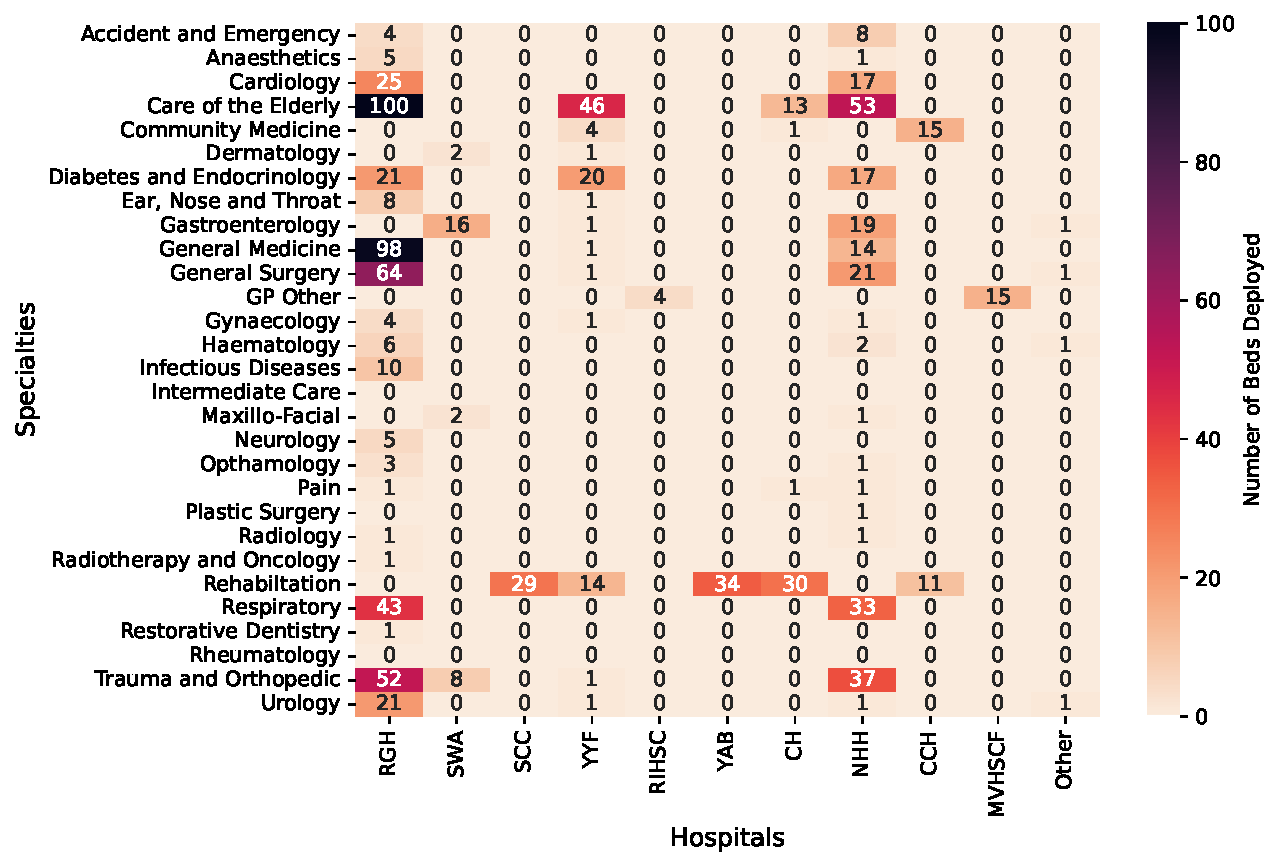
\includegraphics[scale=0.4]{Figures - Heatmaps/Fig25.pdf}
  \captionsetup{font={scriptsize}}
  \captionof{figure}{{Heatmap of bed locations for each specialty within each\\ hospital for the deterministic model using the classification tree and \\average LOS for 2017-2018.}}
  \label{fig:app15a}
\end{minipage}%
\begin{minipage}{0.4\linewidth}
  \centering
  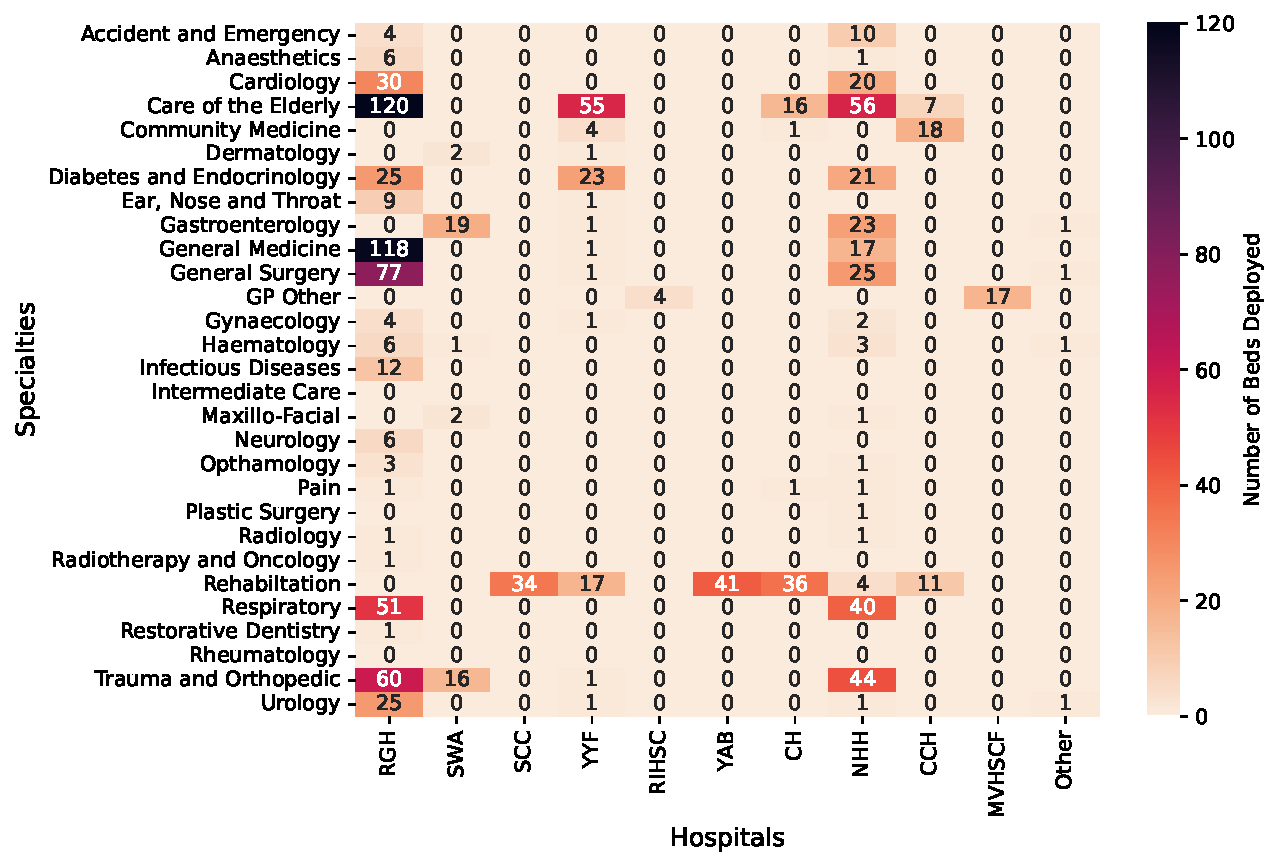
\includegraphics[scale=0.4]{Figures - Heatmaps/Fig26.pdf}  \captionsetup{font={scriptsize}}
  \captionof{figure}{Heatmap of bed locations for each specialty within each\\ hospital for the two-stage stochastic model using the classification tree and \\average LOS for 2017-2018.}
  \label{fig:app15b}
\end{minipage}
\end{figure}

\begin{figure}[h!]
\centering
\begin{minipage}{0.4\linewidth}
  \centering
  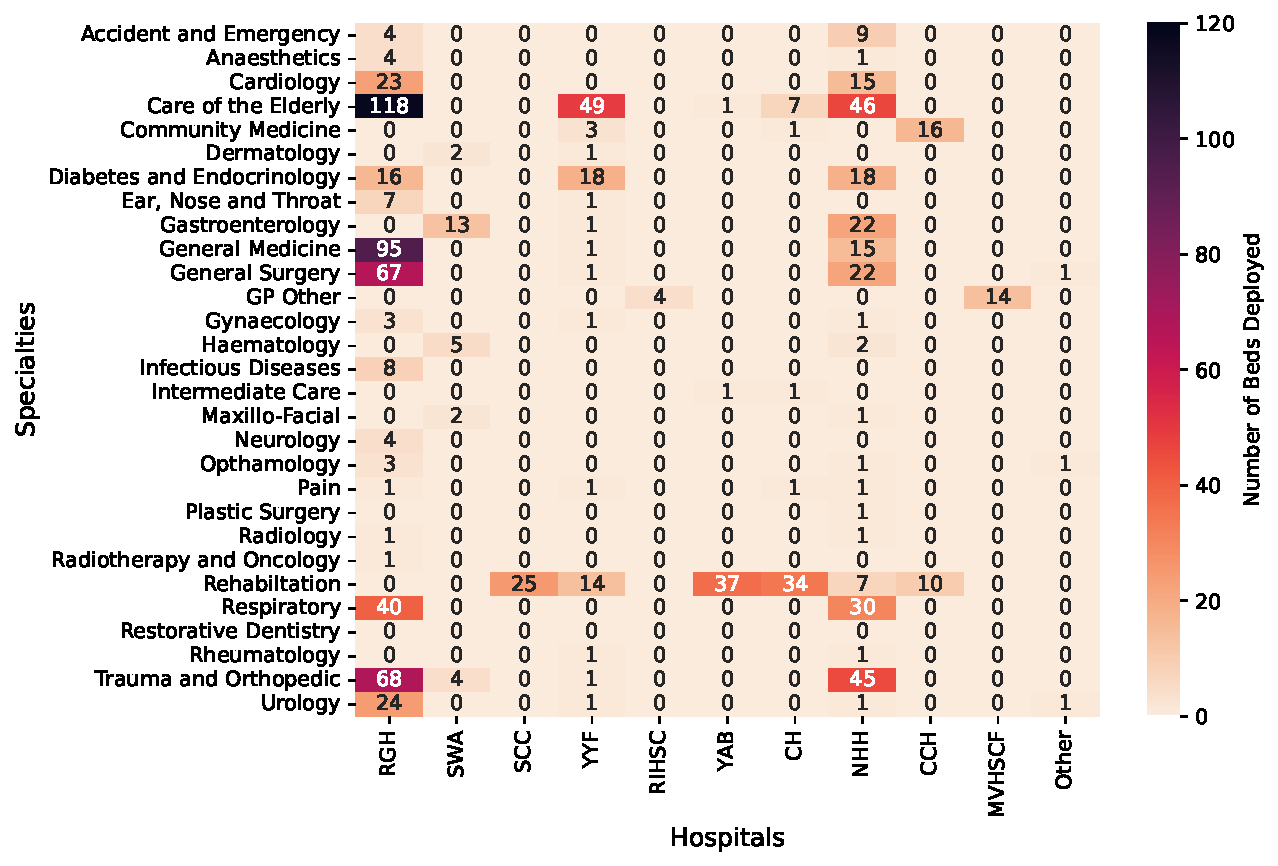
\includegraphics[scale=0.4]{Figures - Heatmaps/Fig27.pdf}
\captionsetup{font={scriptsize}}
  \captionof{figure}{{Heatmap of bed locations for each specialty within each\\ hospital for the deterministic model using the classification tree and \\average LOS for 2018-2019.}}
  \label{fig:app16a}
\end{minipage}%
\begin{minipage}{0.4\linewidth}
  \centering
  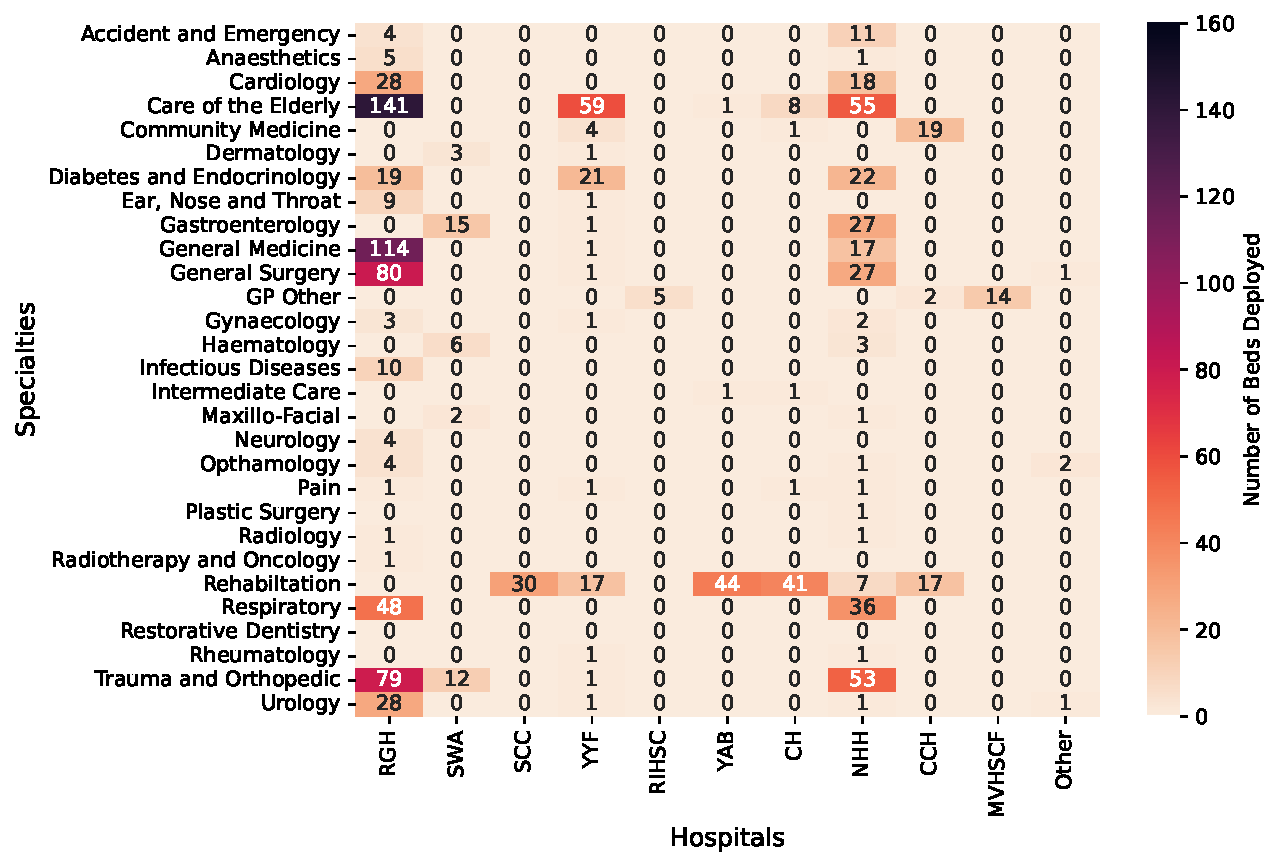
\includegraphics[scale=0.4]{Figures - Heatmaps/Fig28.pdf}
  \captionsetup{font={scriptsize}}
  \captionof{figure}{{Heatmap of bed locations for each specialty within each\\ hospital for the two-stage stochastic model using the classification tree and \\average LOS for 2018-2019.}}
  \label{fig:app16b}
\end{minipage}
\end{figure}

\begin{figure}[h!]
\centering
\begin{minipage}{0.4\linewidth}
  \centering
  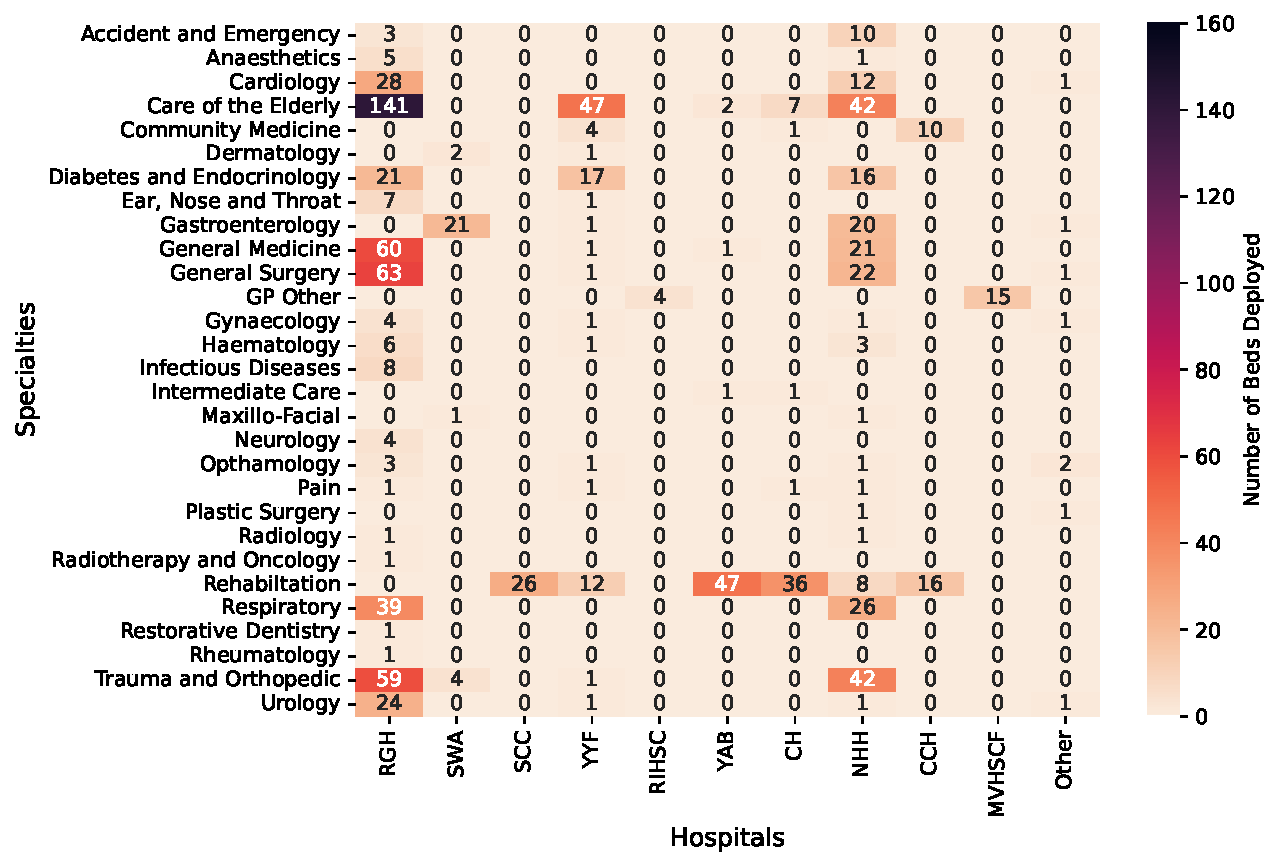
\includegraphics[scale=0.4]{Figures - Heatmaps/Fig29.pdf}
\captionsetup{font={scriptsize}}
  \captionof{figure}{{Heatmap of bed locations for each specialty within each\\ hospital for the deterministic model using the classification tree and \\average LOS for 2019-2020.}}
  \label{fig:app17a}
\end{minipage}%
\begin{minipage}{0.4\linewidth}
  \centering
  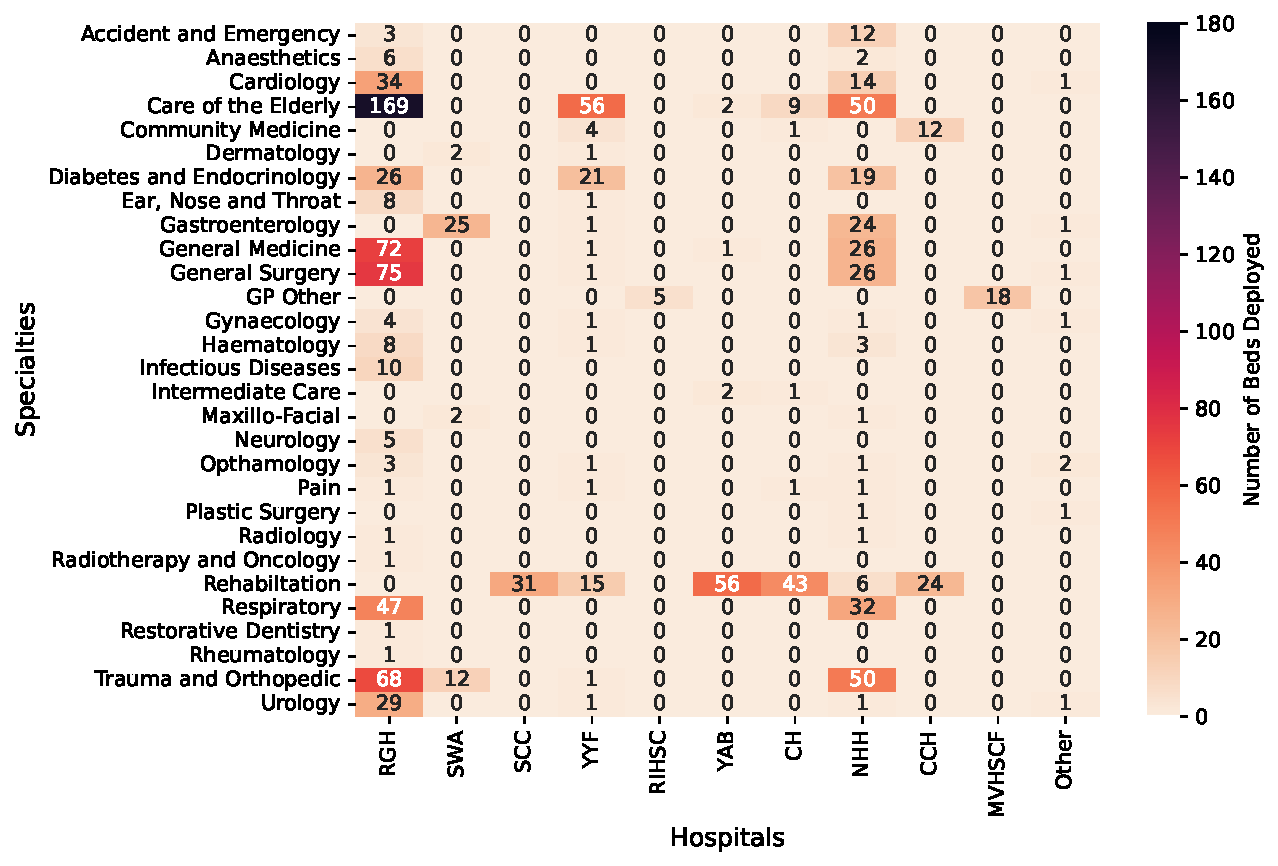
\includegraphics[scale=0.4]{Figures - Heatmaps/Fig30.pdf}
  \captionsetup{font={scriptsize}}
  \captionof{figure}{{Heatmap of bed locations for each specialty within each\\ hospital for the two-stage stochastic model using the classification tree and \\average LOS for 2019-2020.}}
  \label{fig:app17b}
\end{minipage}
\end{figure}
\end{landscape}

\begin{landscape}
    \begin{table}[h!]
    \centering\scalebox{0.8}{
    \begin{tabular}{lcccccccccccccccccc}\toprule
\multirow{2}{*}{\textbf{Specialty}}& \multicolumn{3}{c}{\textbf{Region 1}} & \multicolumn{3}{c}{\textbf{Region 2}}& \multicolumn{3}{c}{\textbf{Region 3}}\\\cmidrule(lr){2-4} \cmidrule(lr){5-7}\cmidrule(lr){8-10}
& \textbf{2017-2018} & \textbf{2018-2019} & \textbf{2019-2020} & \textbf{2017-2018} & \textbf{2018-2019} & \textbf{2019-2020} & \textbf{2017-2018} & \textbf{2018-2019} & \textbf{2019-2020} \\\midrule
Accident \& Emergency&	3.2546&	3.3498&	2.2753&	0.0000&	0.0000&	0.0000&	0.0000&	0.0000&	0.0000\\
Anaesthetics&	4.5748&	3.6941&	4.2057&	0.0000&	0.0000&	0.0000&	0.0000&	0.0000&	0.0000\\
Cardiology&	24.8467&	22.1565&	27.8232&	0.0000&	0.0000&	0.0000&	0.0000&	0.0000&	0.0000\\
Care of the Elderly&	101.8083&	114.9121&	139.8770&	46.1980&	47.9158&	45.7555&	0.0000&	0.1435&	1.5595\\
Community Medicine	&0.0000&	0.0000&	0.0000&	3.1874&	2.9051&	3.2631&	0.0000&	0.0000&	0.0000\\
Dermatology&	1.5243&	1.6713&	1.7106&	0.2269&	0.2859&	0.3767&	0.0000&	0.0000&	0.0000\\
Diabetes and Endocrinology&	21.1122&	14.8840&	20.8111&	19.5744&	17.0001&	16.6421&	0.0000&	0.0000&	0.0000\\
Ear Nose \& Throat&	7.8616&	6.8260&	6.1524&	0.0430&	0.0120&	0.0054&	0.0000&	0.0000&	0.0000\\
Gastroenterology&	15.8905&	11.7729&	20.3049&	0.6772&	0.4819&	0.8694&	0.0000&	0.0000&	0.0000\\
General Medicine	&103.9455&	95.2600&	53.5851&	0.2227&	0.4430&	0.7331&	0.0000&	0.0000&	0.0209\\
General Surgery	&64.8113&	65.3150&	61.9319&	0.3083&	0.2920&	0.4636&	0.0000&	0.0000&	0.0000\\
GP Other	&0.0000&	0.0000&	0.0000&	3.1499&	3.4789&	3.5531&	0.0000&	0.0000&	0.0000\\
Gynaecology&	2.9168&	2.5419&	3.1850&	0.3355&	0.1718&	0.1331&	0.0000&	0.0000&	0.0000\\
Haematology&	5.9642&	4.4035&	6.0321&	0.0000&	0.0000&	0.1848&	0.0000&	0.0000&	0.0000\\
Infectious Diseases	&9.5621&	7.4241&	7.5776&	0.0000&	0.0000&	0.0000&	0.0000&	0.0000&	0.0000\\
Intermediate Care	&0.0000&	0.0000&	0.0000&	0.0000&	0.0000&	0.0000&	0.0000&	0.0359&	0.8339\\
Maxillo-Facial&	1.4029&	1.3015&	0.9645&	0.0000&	0.0000&	0.0000&	0.0000&	0.0000&	0.0000\\
Neurology&	4.3873&	3.2286&	3.3727&	0.0000&	0.0000&	0.0000&	0.0000&	0.0000&	0.0000\\
Ophthalmology&	2.4090&	2.2876&	2.7137&	0.0000&	0.0000&	0.0363&	0.0000&	0.0000&	0.0000\\
Pain&	0.0307&	0.0305&	0.0363&	0.0000&	0.0054&	0.0038&	0.0000&	0.0000&	0.0000\\
Plastic Surgery	&0.0000&	0.0000&	0.0000&	0.0000&	0.0000&	0.0000&	0.0000&	0.0000&	0.0000\\
Radiology&	0.0018&	0.0369&	0.0392&	0.0000&	0.0000&	0.0000&	0.0000&	0.0000&	0.0000\\
Radiotherapy and Oncology&	0.0060&	0.0024&	0.0013&	0.0000&	0.0000&	0.0000&	0.0000&	0.0000&	0.0000\\
Rehabilitation&	29.0237&	24.4600&	25.3794&	13.9119&	13.6287&	11.7833&	34.4235&	35.5782&	46.0456\\
Respiratory&	42.8309&	38.2732&	37.8883&	0.0000&	0.0000&	0.0000&	0.0000&	0.0000&	0.0000\\
Restorative Dentistry	&0.0003&	0.0000&	0.0004&	0.0000&	0.0000&	0.0000&	0.0000&	0.0000&	0.0000\\
Rheumatology&	0.0000&	0.0000&	0.0004&	0.0000&	0.1435&	0.0000&	0.0000&	0.0000&	0.0000\\
Trauma \& Orthopaedic&	61.4394&	70.5687&	61.4178&	0.2786&	0.3522&	0.2350&	0.0000&	0.0000&	0.0000\\
Urology&	20.3556&	23.2087&	23.0969&	0.0141&	0.0950&	0.0083&	0.0000&	0.0000&	0.0000\\

\bottomrule
\end{tabular}  } 
\caption{The daily bed demands for each specialty for regions one, two and three within ABUHB for three individual years’ worth of patient admissions, using the classification tree and the yearly average LOS.}
%\caption{Regions One, Two and Three Daily Demands for Three Individual Years of ABUHB Patient Admissions to Four Decimal Places - Classification Tree and Yearly Average LOS}
    \label{apptab:LinkedDemands8a}
\end{table}  



\begin{table}[h!]
    \centering\scalebox{0.8}{
    \begin{tabular}{lcccccccccccccccccc}\toprule
\multirow{2}{*}{\textbf{Specialty}}& \multicolumn{3}{c}{\textbf{Region 4}} & \multicolumn{3}{c}{\textbf{Region 4}}& \multicolumn{3}{c}{\textbf{Region 6}}\\\cmidrule(lr){2-4} \cmidrule(lr){5-7}\cmidrule(lr){8-10}
& \textbf{2017-2018} & \textbf{2018-2019} & \textbf{2019-2020} & \textbf{2017-2018} & \textbf{2018-2019} & \textbf{2019-2020} & \textbf{2017-2018} & \textbf{2018-2019} & \textbf{2019-2020} \\\midrule


Accident \& Emergency&	0.0000&	0.0000&	0.0000&	7.6680&	8.6804&	9.9681&	0.0000&	0.0000&	0.0000\\
Anaesthetics&	0.0000&	0.0000&	0.0000&	0.4638&	0.4268&	0.9722&	0.0000&	0.0000&	0.0000\\
Cardiology&	0.0000&	0.0000&	0.0000&	16.1539&	14.2806&	11.1400&	0.0000&	0.0000&	0.0011\\
Care of the Elderly&	12.5281&	6.5938&	6.8223&	52.3094&	45.1508&	41.2107&	0.0000&	0.0000&	0.0000\\
Community Medicine	&0.4234&	0.2117&	0.4222&	14.1831&	15.4549&	9.9576&	0.0000&	0.0000&	0.0000\\
Dermatology&	0.0000&	0.0000&	0.0000&	0.0000&	0.0000&	0.0000&	0.0000&	0.0000&	0.0000\\
Diabetes and Endocrinology&	0.0000&	0.0000&	0.0000&	16.6698&	17.8823&	15.3511&	0.0000&	0.0000&	0.0000\\
Ear Nose \& Throat&	0.0000&	0.0000&	0.0000&	0.0000&	0.0000&	0.0000&	0.0000&	0.0000&	0.0000\\
Gastroenterology&	0.0000&	0.0000&	0.0000&	18.7998&	21.9374&	19.9778&	0.3047&	0.0000&	0.0022\\
General Medicine	&0.0000&	0.0000&	0.0000&	13.9936&	14.0130&	20.9445&	0.0000&	0.0000&	0.0000\\
General Surgery	&0.0000&	0.0000&	0.0000&	20.4583&	21.6905&	21.4020&	0.0011&	0.0011&	0.0011\\
GP Other	&0.0000&	0.0000&	0.0000&	14.1544&	13.2848&	14.3738&	0.0000&	0.0000&	0.0000\\
Gynaecology&	0.0000&	0.0000&	0.0000&	0.9738&	0.9246&	0.6943&	0.0000&	0.0000&	0.0011\\
Haematology&	0.0000&	0.0000&	0.0000&	1.8249&	1.7582&	2.0842&	0.0011&	0.0000&	0.0000\\
Infectious Diseases	&0.0000&	0.0000&	0.0000&	0.0000&	0.0000&	0.0000&	0.0000&	0.0000&	0.0000\\
Intermediate Care	&0.0000&	0.3333&	0.3699&	0.0000&	0.0000&	0.0000&	0.0000&	0.0000&	0.0000\\
Maxillo-Facial&	0.0000&	0.0000&	0.0000&	0.1061&	0.0747&	0.0969&	0.0000&	0.0000&	0.0000\\
Neurology&	0.0000&	0.0000&	0.0000&	0.0000&	0.0000&	0.0000&	0.0000&	0.0000&	0.0000\\
Ophthalmology&	0.0000&	0.0000&	0.0000&	0.3948&	0.4613&	0.4636&	0.0000&	0.9640&	1.2960\\
Pain&	0.0166&	0.0110&	0.0176&	0.0519&	0.0442&	0.0396&	0.0000&	0.0000&	0.0000\\
Plastic Surgery	&0.0000&	0.0000&	0.0000&	0.0521&	0.0464&	0.0462&	0.0000&	0.0000&	0.0011\\
Radiology&	0.0000&	0.0000&	0.0000&	0.0091&	0.0011&	0.0225&	0.0000&	0.0000&	0.0000\\
Radiotherapy and Oncology&	0.0000&	0.0000&	0.0000&	0.0000&	0.0000&	0.0000&	0.0000&	0.0000&	0.0000\\
Rehabilitation&	29.5478&	33.4318&	35.5989&	10.7206&	16.2437&	23.0764&	0.0000&	0.0000&	0.0000\\
Respiratory&	0.0000&	0.0000&	0.0000&	32.7445&	29.8673&	25.8748&	0.0000&	0.0000&	0.0000\\
Restorative Dentistry	&0.0000&	0.0000&	0.0000&	0.0000&	0.0000&	0.0000&	0.0000&	0.0000&	0.0000\\
Rheumatology&	0.0000&	0.0000&	0.0000&	0.0000&	0.0215&	0.0000&	0.0000&	0.0000&	0.0000\\
Trauma \& Orthopaedic&	0.0000&	0.0000&	0.0000&	36.3659&	44.0053&	41.3888&	0.0000&	0.0000&	0.0000\\
Urology&	0.0000&	0.0000&	0.0000&	0.5179&	0.4967&	0.5494&	0.0210&	0.0169&	0.0226\\
\bottomrule
\end{tabular}  } 
\caption{The daily bed demands for each specialty for regions four, five and six within ABUHB for three individual years’ worth of patient admissions, using the classification tree and the yearly average LOS.}
    \label{apptab:LinkedDemands8b}
\end{table}

    
\end{landscape}

\begin{landscape}
    
\begin{figure}[h!]
\centering
\begin{minipage}{0.4\linewidth}
  \centering
  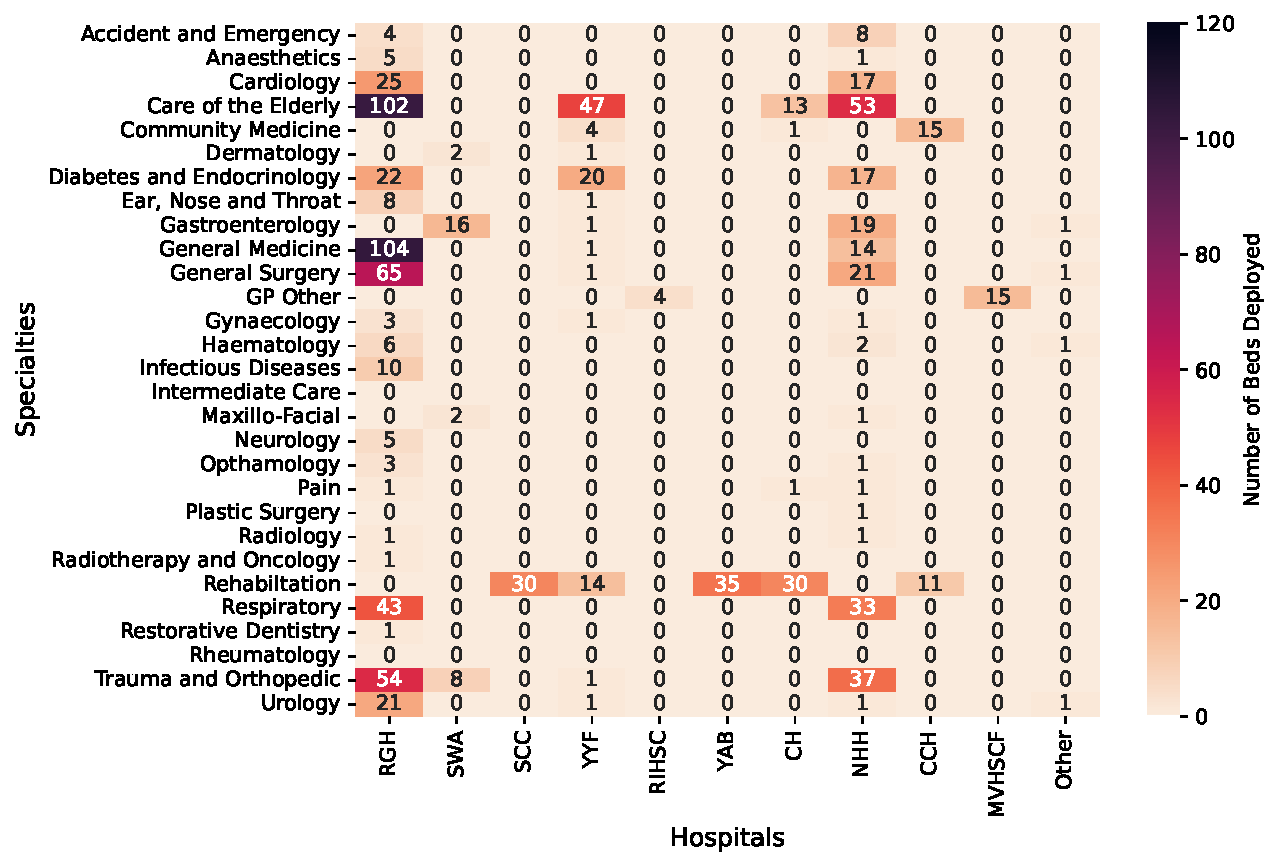
\includegraphics[scale=0.4]{Figures - Heatmaps/Fig31.pdf}
  \captionsetup{font={scriptsize}}
  \captionof{figure}{{Heatmap of bed locations for each specialty within each\\ hospital for the deterministic model using the classification tree and \\average year LOS for 2017-2018.}}
  \label{fig:app18a}
\end{minipage}%
\begin{minipage}{0.4\linewidth}
  \centering
  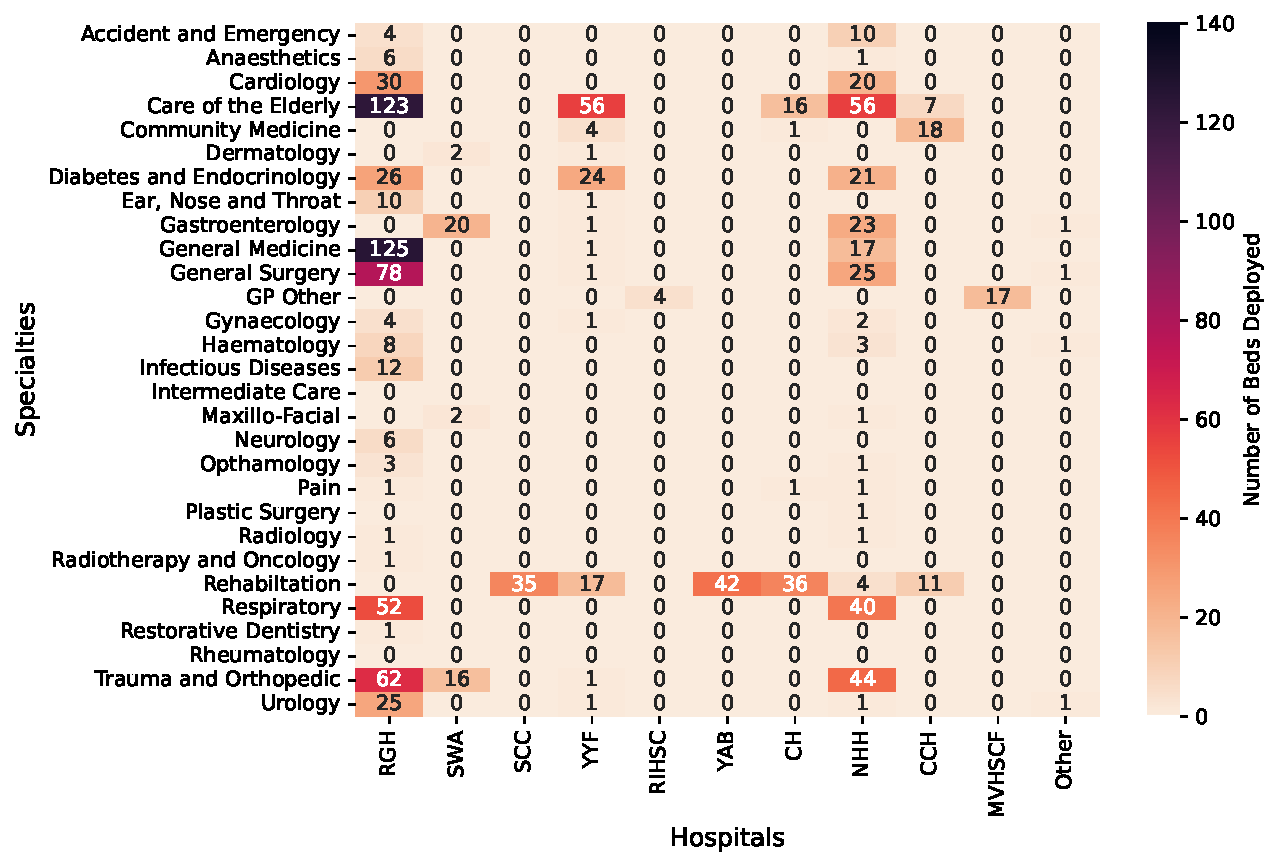
\includegraphics[scale=0.4]{Figures - Heatmaps/Fig32.pdf}  \captionsetup{font={scriptsize}}
  \captionof{figure}{{Heatmap of bed locations for each specialty within each\\ hospital for the two-stage stochastic model using the classification tree and \\average year LOS for 2017-2018.}}
  \label{fig:app18b}
\end{minipage}
\end{figure}

\begin{figure}[h!]
\centering
\begin{minipage}{0.4\linewidth}
  \centering
  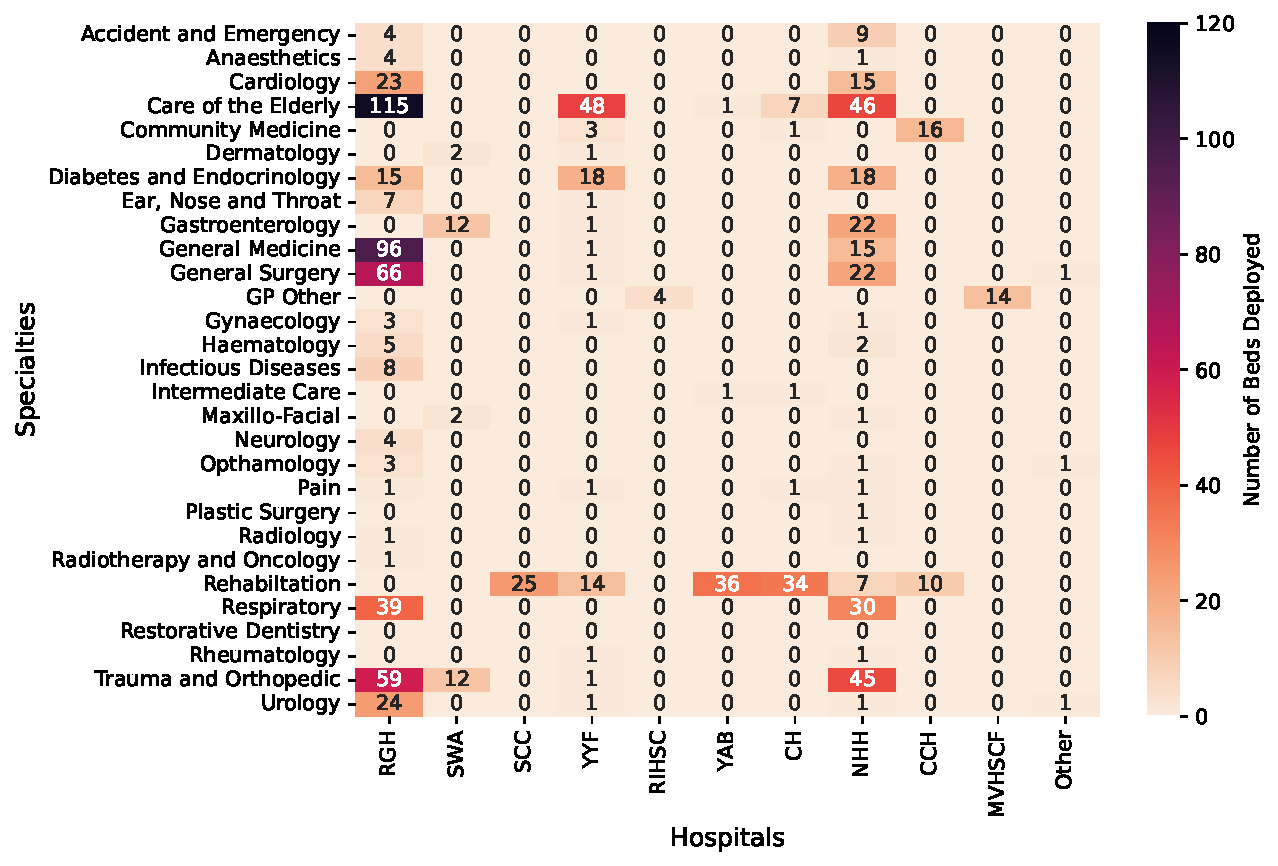
\includegraphics[scale=0.4]{Figures - Heatmaps/Fig33.pdf}
\captionsetup{font={scriptsize}}
  \captionof{figure}{{Heatmap of bed locations for each specialty within each\\ hospital for the deterministic model using the classification tree and \\average year LOS for 2018-2019.}}
  \label{fig:app19a}
\end{minipage}%
\begin{minipage}{0.4\linewidth}
  \centering
  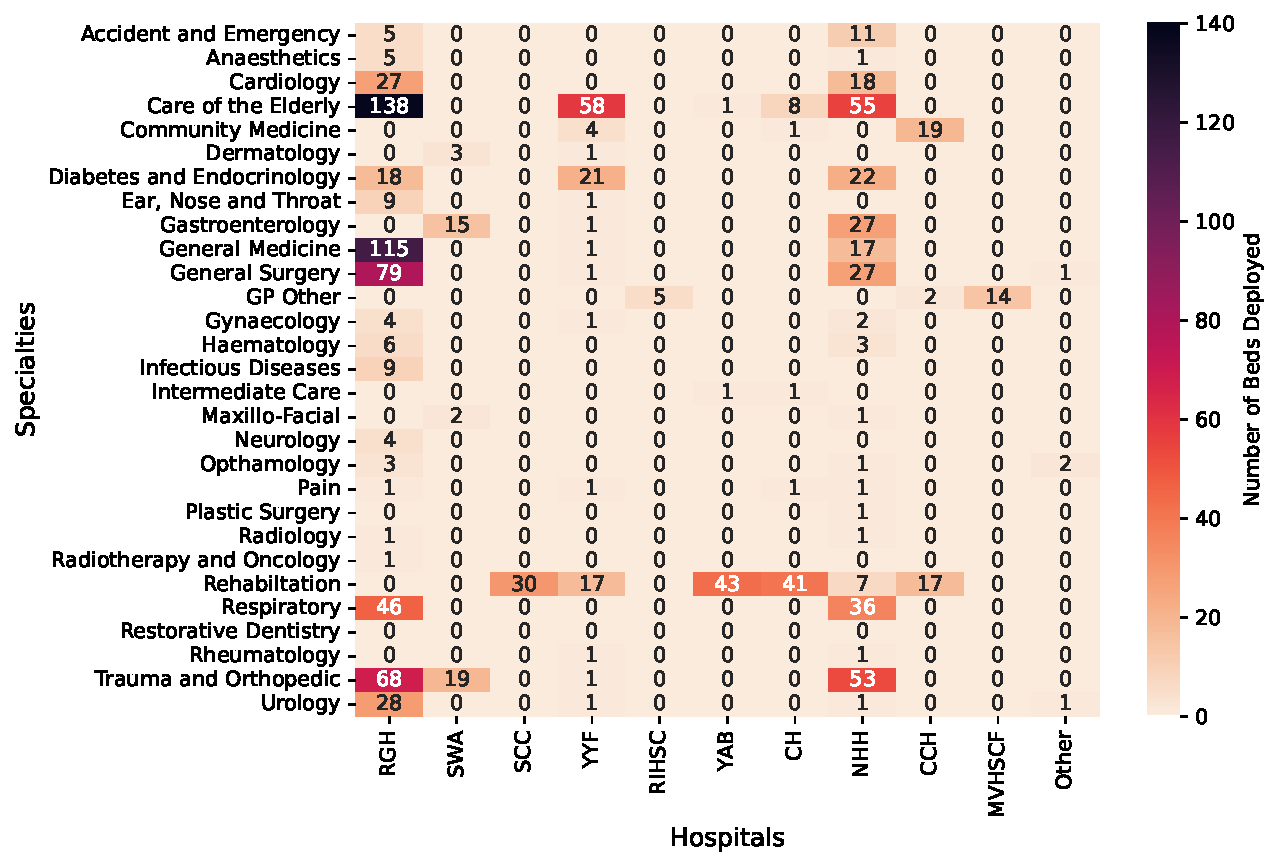
\includegraphics[scale=0.4]{Figures - Heatmaps/Fig34.pdf}
  \captionsetup{font={scriptsize}}
  \captionof{figure}{{Heatmap of bed locations for each specialty within each\\ hospital for the two-stage stochastic model using the classification tree and \\average year LOS for 2018-2019.}}
  \label{fig:app19b}
\end{minipage}
\end{figure}

\begin{figure}[h!]
\centering
\begin{minipage}{0.4\linewidth}
  \centering
  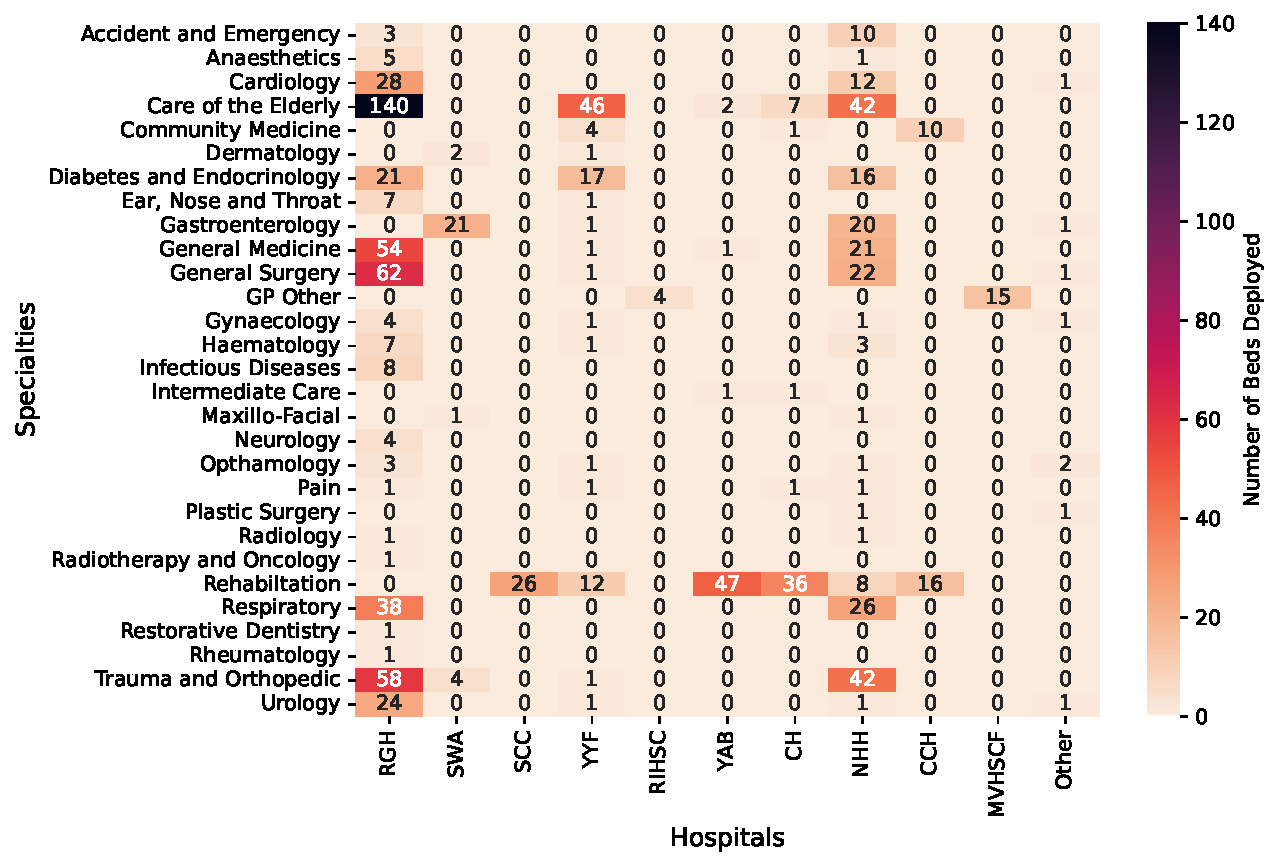
\includegraphics[scale=0.4]{Figures - Heatmaps/Fig35.pdf}
\captionsetup{font={scriptsize}}
  \captionof{figure}{{Heatmap of bed locations for each specialty within each\\ hospital for the deterministic model using the classification tree and \\average year LOS for 2019-2020.}}
  \label{fig:app20a}
\end{minipage}%
\begin{minipage}{0.4\linewidth}
  \centering
  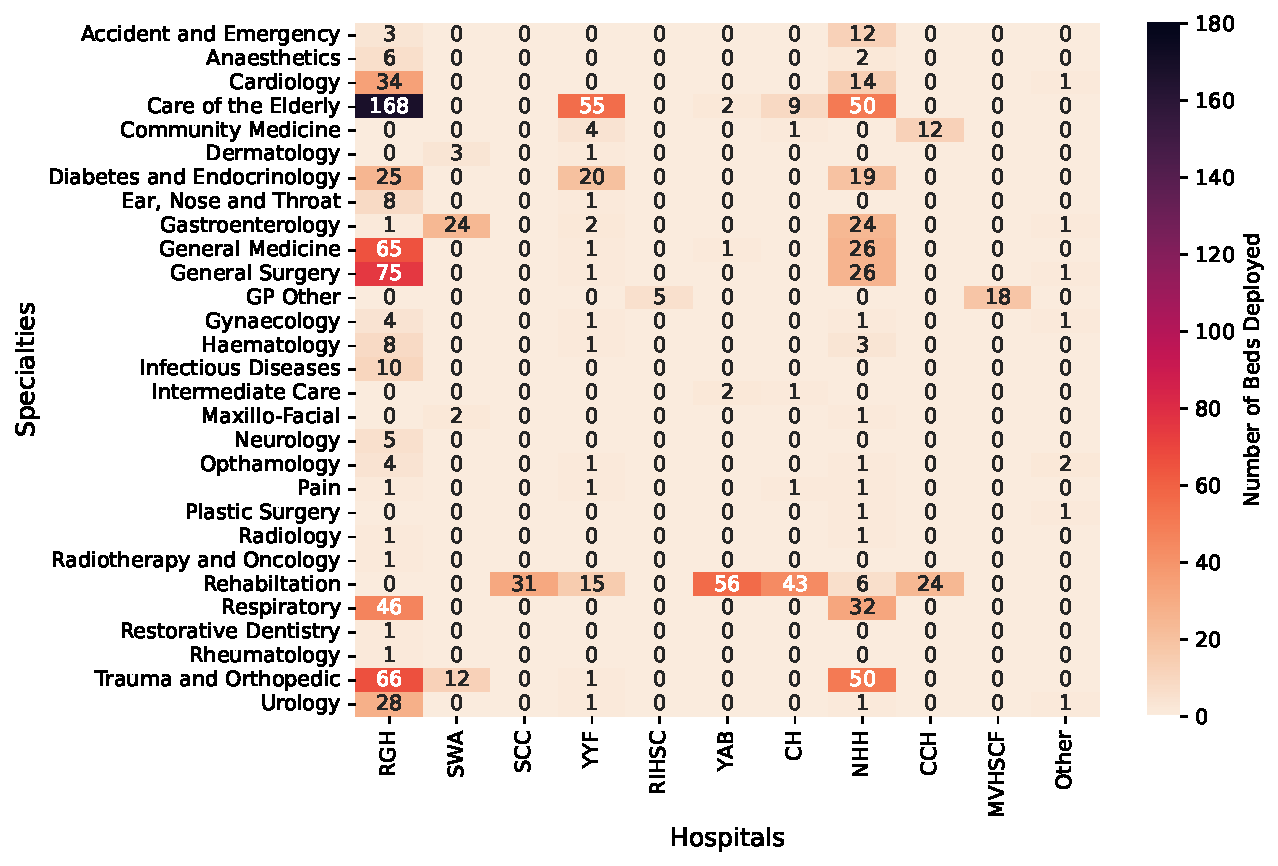
\includegraphics[scale=0.4]{Figures - Heatmaps/Fig36.pdf}
  \captionsetup{font={scriptsize}}
  \captionof{figure}{{Heatmap of bed locations for each specialty within each\\ hospital for the two-stage stochastic model using the classification tree and \\average year LOS for 2019-2020.}} 
  \label{fig:app20b}
\end{minipage}
\end{figure}
\end{landscape}

\section{Classification Trees - Specific LOS}

\begin{table}[h!]
    \centering\scalebox{0.78}{
    \begin{tabular}{lcccccc} \toprule
\textbf{Specialty} &	\textbf{Region 1}	&\textbf{Region 2}&	\textbf{Region 3}	&\textbf{Region 4}	&\textbf{Region 5}&	\textbf{Region 6} \\\midrule
Accident \& Emergency&	2.1168&	0.0000&	0.0000&	0.0000&	9.1761&	0.0000\\
Anaesthetics&	4.5894&	0.0000&	0.0000&	0.0000&	0.7719&	0.0000\\
Cardiology&	15.5265&	0.0000&	0.0000&	0.0000&	9.7901&	0.0000\\
Care of the Elderly&	93.9772&	57.7354&	0.7573&	8.7856&	46.4398&	0.0000\\
Community Medicine&	0.0000&	7.0073&	0.0000&	0.3139&	13.0137&	0.0000\\
Dermatology&	2.2591&	0.0000&	0.0000&	0.0000&	0.0000&	0.0000\\
Diabetes and Endocrinology&	14.4489&	21.2409&	0.0000&	0.0000&	17.2290&	0.0000\\
Ear Nose \& Throat&	3.1104&	0.0009&	0.0000&	0.0000&	0.0000&	0.0000\\
Gastroenterology&	12.3120&	0.0985&	0.0000&	0.0000&	19.7765&	0.0009\\
General Medicine&	84.4854&	0.9818&	0.0119&	0.0000&	14.1013&	0.0000\\
General Surgery&	45.5192&	0.2318&	0.0000&	0.0000&	21.3011&	0.0000\\
GP Other&	0.0000&	9.8723&	0.0000&	0.0000&	15.3102&	0.0000\\
Gynaecology&	2.0046&	0.0721&	0.0000&	0.0000&	1.0766&	0.0000\\
Haematology&	2.7792&	0.0265&	0.0000&	0.0000&	1.1332&	0.0000\\
Infectious Diseases&	7.1195&	0.0000&	0.0000&	0.0000&	0.0000&	0.0000\\
Intermediate Care&	0.0000&	0.0000&	0.3449&	0.3239&	0.0000&	0.0000\\
Maxillo-Facial&	1.0547&	0.0000&	0.0000&	0.0000&	0.0027&	0.0000\\
Neurology&	1.5620&	0.0000&	0.0000&	0.0000&	0.0000&	0.0000\\
Ophthalmology&	1.3704&	0.0027&	0.0000&	0.0000&	0.0009&	0.0036\\
Pain&	0.0018&	0.0000&	0.0000&	0.0018&	0.0000&	0.0000\\
Plastic Surgery&	0.0000&	0.0000&	0.0000&	0.0000&	0.0137&	0.0000\\
Radiology&	0.0100&	0.0000&	0.0000&	0.0000&	0.0000&	0.0000\\
Radiotherapy and Oncology&	0.2245&	0.0000&	0.0000&	0.0000&	0.0000&	0.0000\\
Rehabilitation&	63.0173&	33.0922&	69.4863&	32.1077&	24.5538&	0.0000\\
Respiratory&	29.4717&	0.0000&	0.0000&	0.0000&	27.7290&	0.0000\\
Restorative Dentistry&	0.0000&	0.0000&	0.0000&	0.0000&	0.0000&	0.0000\\
Rheumatology&	0.0000&	0.0000&	0.0000&	0.0000&	0.0128&	0.0000\\
Trauma \& Orthopaedic&	59.1807&	0.2956&	0.0000&	0.0000&	40.6989&	0.0000\\
Urology&	11.3257&	0.0036&	0.0000&	0.0000&	0.0255&	0.0401\\


\bottomrule

    \end{tabular}}
    \caption{The daily bed demands for each specialty grouped by regions within ABUHB for three years’ worth of patient admissions, using the classification tree and specific LOS.}
    %\caption{Linked Predictive and Prescriptive Demands - Classification Tree and Specific LOS - Three Years' Worth of Data}
    \label{apptab:LinkedDemands9}
\end{table}

\begin{figure}[h!]
    \centering
    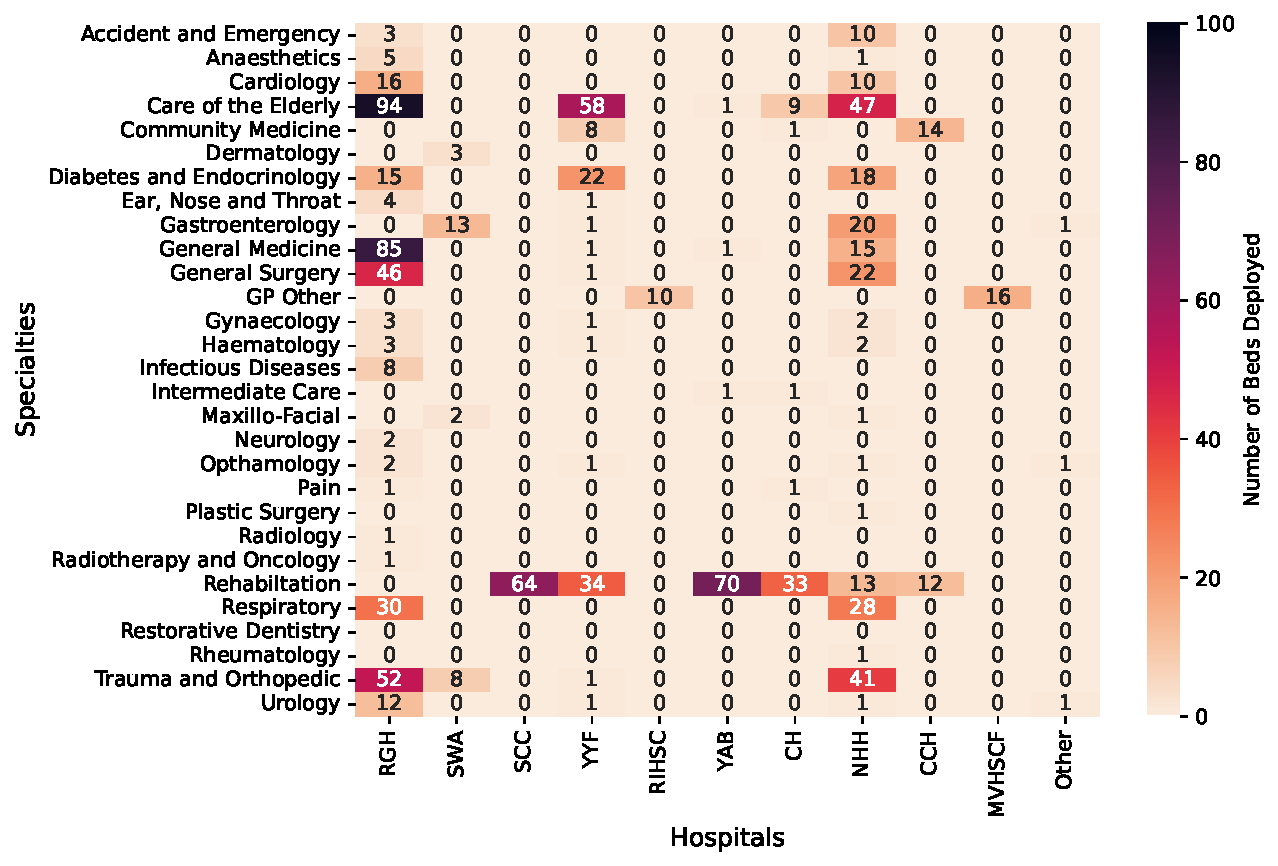
\includegraphics[scale=0.55]{Figures - Heatmaps/Fig37.pdf}
\caption{Heatmap of bed locations for each specialty within each hospital for the deterministic model using the classification tree and specific LOS over three years' worth of data.}
    \label{fig:app14a}
\end{figure}
\begin{figure}[h!]
    \centering
    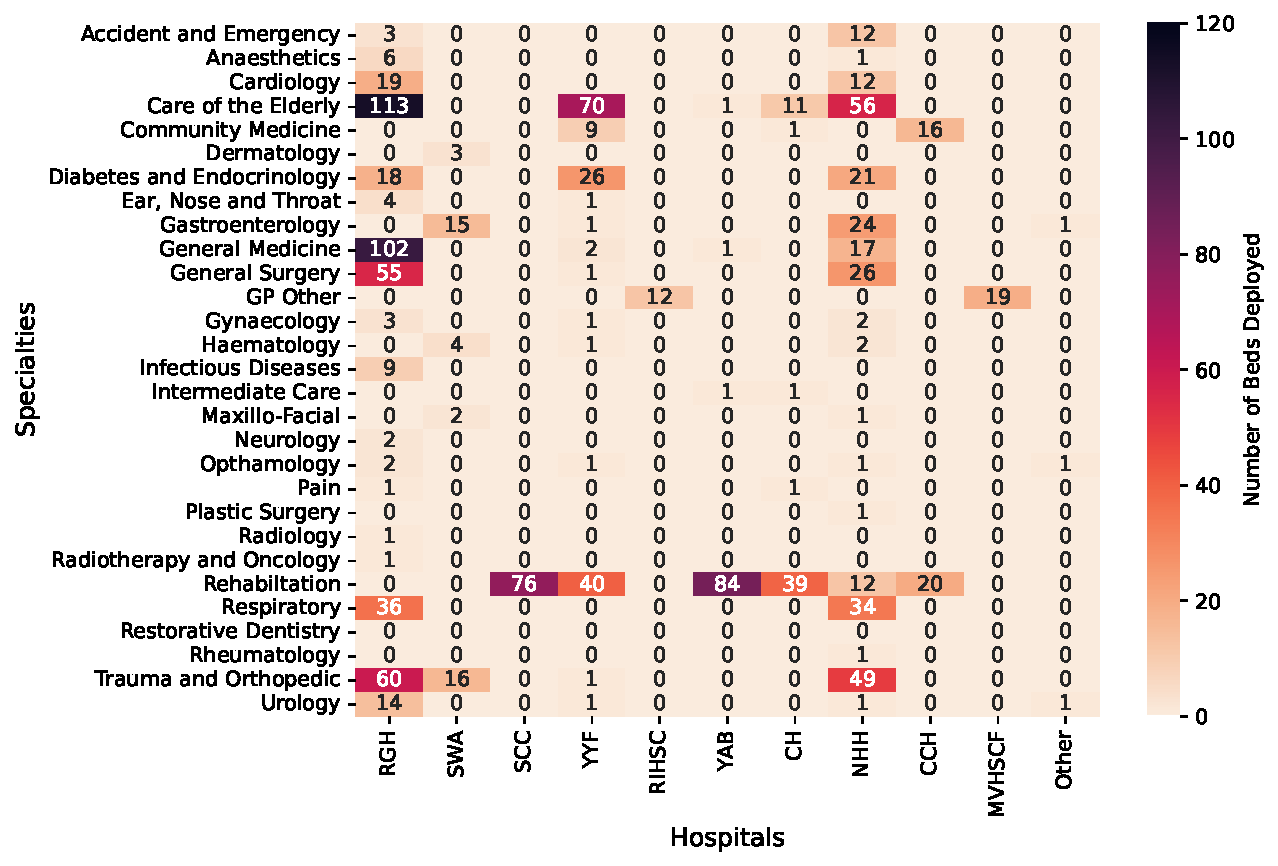
\includegraphics[scale=0.55]{Figures - Heatmaps/Fig38.pdf}
\caption{Heatmap of bed locations for each specialty within each hospital for the two-stage stochastic model using the classification tree and specific LOS over three years' worth of data.}
    \label{fig:app14b}
\end{figure}

\begin{landscape}

    \begin{table}[h!]
    \centering\scalebox{0.8}{
    \begin{tabular}{lcccccccccccccccccc}\toprule
\multirow{2}{*}{\textbf{Specialty}}& \multicolumn{3}{c}{\textbf{Region 1}} & \multicolumn{3}{c}{\textbf{Region 2}}& \multicolumn{3}{c}{\textbf{Region 3}}\\\cmidrule(lr){2-4} \cmidrule(lr){5-7}\cmidrule(lr){8-10}
& \textbf{2017-2018} & \textbf{2018-2019} & \textbf{2019-2020} & \textbf{2017-2018} & \textbf{2018-2019} & \textbf{2019-2020} & \textbf{2017-2018} & \textbf{2018-2019} & \textbf{2019-2020} \\\midrule
Accident \& Emergency&	2.2932&	2.2000&	1.8579&	0.0000&	0.0000&	0.0000&	0.0000&	0.0000&	0.0000\\
Anaesthetics&	4.4932&	4.4712&	4.8033&	0.0000&	0.0000&	0.0000&	0.0000&	0.0000&	0.0000\\
Cardiology&	16.7918&	14.0630&	15.7240&	0.0000&	0.0000&	0.0000&	0.0000&	0.0000&	0.0000\\
Care of the Elderly&	76.4575&	88.0658&	117.3443&	55.8247&	58.4877&	58.8907&	0.0000&	0.4000&	1.8689\\
Community Medicine&	0.0000&	0.0000&	0.0000&	7.1671&	6.1014&	7.7514&	0.0000&	0.0000&	0.0000\\
Dermatology&	2.6877&	1.9918&	2.0984&	0.0000&	0.0000&	0.0000&	0.0000&	0.0000&	0.0000\\
Diabetes and Endocrinology&	16.5863&	11.4356&	15.3224&	24.7041&	19.8055&	19.2186&	0.0000&	0.0000&	0.0000\\
Ear Nose \& Throat&	2.9616&	3.6192&	2.7514&	0.0027&	0.0000&	0.0000&	0.0000&	0.0000&	0.0000\\
Gastroenterology&	11.4438&	9.8219&	15.6612&	0.1260&	0.0219&	0.1475&	0.0000&	0.0000&	0.0000\\
General Medicine&	105.6712&	96.0603&	51.8142&	0.2877&	1.1479&	1.5082&	0.0000&	0.0000&	0.0355\\
General Surgery&	47.9068&	45.3479&	43.3087&	0.2000&	0.2301&	0.2650&	0.0000&	0.0000&	0.0000\\
GP Other&	0.0000&	0.0000&	0.0000&	9.6795&	10.1151&	9.8224&	0.0000&	0.0000&	0.0000\\
Gynaecology&	2.4301&	1.7233&	1.8607&	0.0795&	0.0740&	0.0628&	0.0000&	0.0000&	0.0000\\
Haematology&	3.1096&	2.4384&	2.7896&	0.0000&	0.0000&	0.0792&	0.0000&	0.0000&	0.0000\\
Infectious Diseases&	8.0767&	6.3918&	6.8907&	0.0000&	0.0000&	0.0000&	0.0000&	0.0000&	0.0000\\
Intermediate Care&	0.0000&	0.0000&	0.0000&	0.0000&	0.0000&	0.0000&	0.0000&	0.0082&	1.0246\\
Maxillo-Facial&	1.1068&	0.9178&	1.1393&	0.0000&	0.0000&	0.0000&	0.0000&	0.0000&	0.0000\\
Neurology&	1.4301&	1.5534&	1.7022&	0.0000&	0.0000&	0.0000&	0.0000&	0.0000&	0.0000\\
Ophthalmology&	1.4712&	1.2685&	1.3716&	0.0000&	0.0000&	0.0082&	0.0000&	0.0000&	0.0000\\
Pain&	0.0000&	0.0000&	0.0055&	0.0000&	0.0000&	0.0000&	0.0000&	0.0000&	0.0000\\
Plastic Surgery&	0.0000&	0.0000&	0.0000&	0.0000&	0.0000&	0.0000&	0.0000&	0.0000&	0.0000\\
Radiology&	0.0055&	0.0164&	0.0082&	0.0000&	0.0000&	0.0000&	0.0000&	0.0000&	0.0000\\
Radiotherapy and Oncology&	0.0000&	0.0000&	0.6721&	0.0000&	0.0000&	0.0000&	0.0000&	0.0000&	0.0000\\
Rehabilitation&	64.7671&	63.1151&	61.1749&	34.9123&	34.8384&	29.5355&	69.9671&	65.3863&	73.0956\\
Respiratory&	29.8658&	30.4137&	28.1393&	0.0000&	0.0000&	0.0000&	0.0000&	0.0000&	0.0000\\
Restorative Dentistry&	0.0000&	0.0000&	0.0000&	0.0000&	0.0000&	0.0000&	0.0000&	0.0000&	0.0000\\
Rheumatology&	0.0000&	0.0000&	0.0000&	0.0000&	0.0000&	0.0000&	0.0000&	0.0000&	0.0000\\
Trauma \& Orthopaedic&	56.0082&	60.6164&	60.9126&	0.3808&	0.2712&	0.2350&	0.0000&	0.0000&	0.0000\\
Urology&	10.3671&	12.5726&	11.0383&	0.0027&	0.0055&	0.0027&	0.0000&	0.0000&	0.0000\\

\bottomrule
\end{tabular}  } 
\caption{The daily bed demands for each specialty for regions one, two and three within ABUHB for three individual years’ worth of patient admissions, using the classification tree and the yearly specific LOS.}
    \label{apptab:LinkedDemands10a}
\end{table}  


    \begin{table}[h!]
    \centering\scalebox{0.8}{
    \begin{tabular}{lcccccccccccccccccc}\toprule
\multirow{2}{*}{\textbf{Specialty}}& \multicolumn{3}{c}{\textbf{Region 4}} & \multicolumn{3}{c}{\textbf{Region 5}}& \multicolumn{3}{c}{\textbf{Region 6}}\\\cmidrule(lr){2-4} \cmidrule(lr){5-7}\cmidrule(lr){8-10}
& \textbf{2017-2018} & \textbf{2018-2019} & \textbf{2019-2020} & \textbf{2017-2018} & \textbf{2018-2019} & \textbf{2019-2020} & \textbf{2017-2018} & \textbf{2018-2019} & \textbf{2019-2020} \\\midrule
Accident \& Emergency&	0.0000&	0.0000&	0.0000&	7.6680&	8.6804&	9.9681&	0.0000&	0.0000&	0.0000\\
Anaesthetics&	0.0000&	0.0000&	0.0000&	0.4638&	0.4268&	0.9722&	0.0000&	0.0000&	0.0000\\
Cardiology&	0.0000&	0.0000&	0.0000&	16.1539&	14.2806&	11.1400&	0.0000&	0.0000&	0.0011\\
Care of the Elderly&	12.5281&	6.5938&	6.8223&	52.3094&	45.1508&	41.2107&	0.0000&	0.0000&	0.0000\\
Community Medicine&	0.4234&	0.2117&	0.4222&	14.1831&	15.4549&	9.9576&	0.0000&	0.0000&	0.0000\\
Dermatology&	0.0000&	0.0000&	0.0000&	0.0000&	0.0000&	0.0000&	0.0000&	0.0000&	0.0000\\
Diabetes and Endocrinology&	0.0000&	0.0000&	0.0000&	16.6698&	17.8823&	15.3511&	0.0000&	0.0000&	0.0000\\
Ear Nose \& Throat&	0.0000&	0.0000&	0.0000&	0.0000&	0.0000&	0.0000&	0.0000&	0.0000&	0.0000\\
Gastroenterology&	0.0000&	0.0000&	0.0000&	18.7998&	21.9374&	19.9778&	0.3047&	0.0000&	0.0022\\
General Medicine&	0.0000&	0.0000&	0.0000&	13.9936&	14.0130&	20.9445&	0.0000&	0.0000&	0.0000\\
General Surgery&	0.0000&	0.0000&	0.0000&	20.4583&	21.6905&	21.4020&	0.0011&	0.0011&	0.0011\\
GP Other&	0.0000&	0.0000&	0.0000&	14.1544&	13.2848&	14.3738&	0.0000&	0.0000&	0.0000\\
Gynaecology&	0.0000&	0.0000&	0.0000&	0.9738&	0.9246&	0.6943&	0.0000&	0.0000&	0.0011\\
Haematology&	0.0000&	0.0000&	0.0000&	1.8249&	1.7582&	2.0842&	0.0011&	0.0000&	0.0000\\
Infectious Diseases&	0.0000&	0.0000&	0.0000&	0.0000&	0.0000&	0.0000&	0.0000&	0.0000&	0.0000\\
Intermediate Care&	0.0000&	0.3333&	0.3699&	0.0000&	0.0000&	0.0000&	0.0000&	0.0000&	0.0000\\
Maxillo-Facial&	0.0000&	0.0000&	0.0000&	0.1061&	0.0747&	0.0969&	0.0000&	0.0000&	0.0000\\
Neurology&	0.0000&	0.0000&	0.0000&	0.0000&	0.0000&	0.0000&	0.0000&	0.0000&	0.0000\\
Ophthalmology&	0.0000&	0.0000&	0.0000&	0.3948&	0.4613&	0.4636&	0.0000&	0.9640&	1.2960\\
Pain&	0.0166&	0.0110&	0.0176&	0.0519&	0.0442&	0.0396&	0.0000&	0.0000&	0.0000\\
Plastic Surgery&	0.0000&	0.0000&	0.0000&	0.0521&	0.0464&	0.0462&	0.0000&	0.0000&	0.0011\\
Radiology&	0.0000&	0.0000&	0.0000&	0.0091&	0.0011&	0.0225&	0.0000&	0.0000&	0.0000\\
Radiotherapy and Oncology&	0.0000&	0.0000&	0.0000&	0.0000&	0.0000&	0.0000&	0.0000&	0.0000&	0.0000\\
Rehabilitation&	29.5478&	33.4318&	35.5989&	10.7206&	16.2437&	23.0764&	0.0000&	0.0000&	0.0000\\
Respiratory&	0.0000&	0.0000&	0.0000&	32.7445&	29.8673&	25.8748&	0.0000&	0.0000&	0.0000\\
Restorative Dentistry&	0.0000&	0.0000&	0.0000&	0.0000&	0.0000&	0.0000&	0.0000&	0.0000&	0.0000\\
Rheumatology&	0.0000&	0.0000&	0.0000&	0.0000&	0.0215&	0.0000&	0.0000&	0.0000&	0.0000\\
Trauma \& Orthopaedic&	0.0000&	0.0000&	0.0000&	36.3659&	44.0053&	41.3888&	0.0000&	0.0000&	0.0000\\
Urology&	0.0000&	0.0000&	0.0000&	0.5179&	0.4967&	0.5494&	0.0210&	0.0169&	0.0226\\

\bottomrule
\end{tabular}  } 
\caption{The daily bed demands for each specialty for regions four, five and six within ABUHB for three individual years’ worth of patient admissions, using the classification tree and the yearly specific LOS.}
    \label{apptab:LinkedDemands10b}
\end{table}  
\end{landscape}
\begin{landscape}
    
\begin{figure}[h!]
\centering
\begin{minipage}{0.4\linewidth}
  \centering
  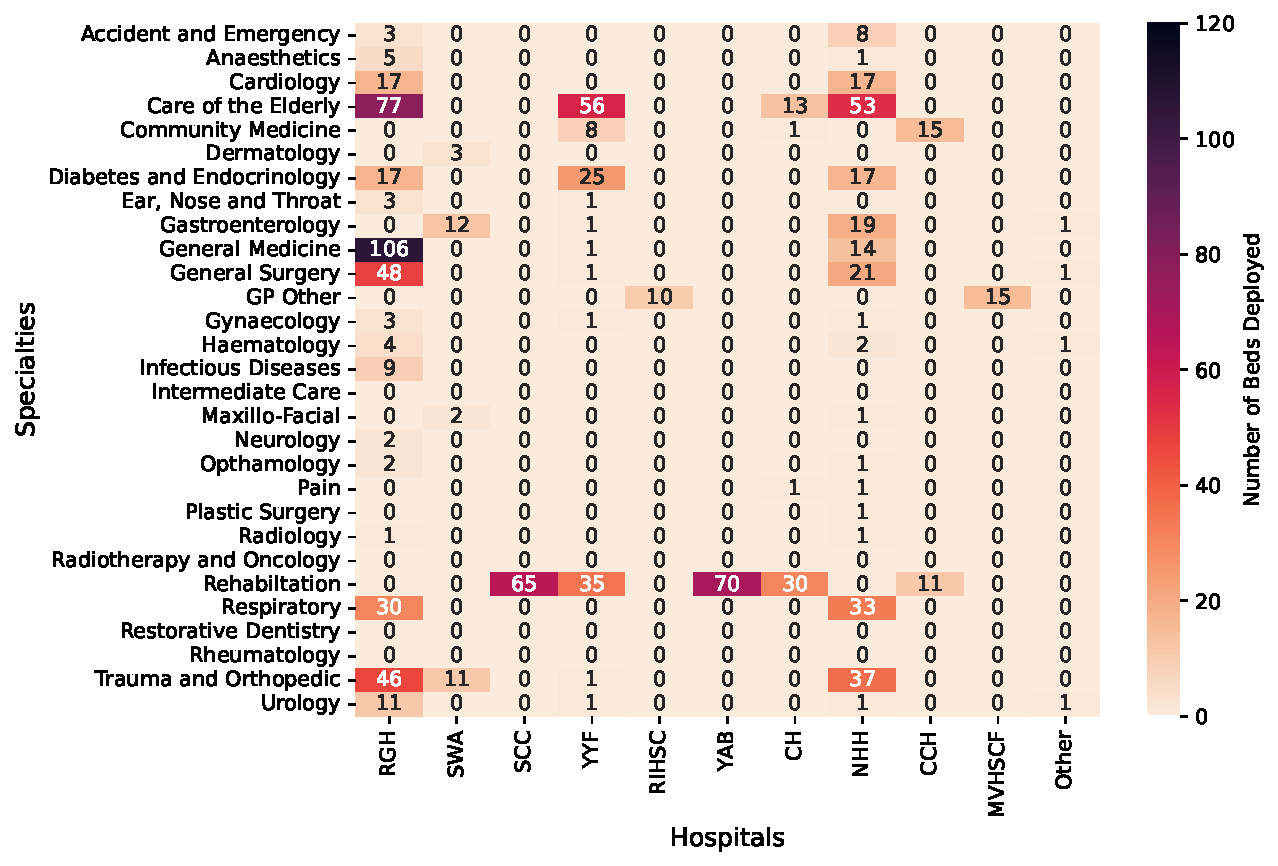
\includegraphics[scale=0.4]{Figures - Heatmaps/Fig39.pdf}
  \captionsetup{font={scriptsize}}
  \captionof{figure}{{Heatmap of bed locations for each specialty within each\\ hospital for the deterministic model using the classification tree and \\specific LOS for 2017-2018.}}
  \label{fig:app22a}
\end{minipage}%
\begin{minipage}{0.4\linewidth}
  \centering
  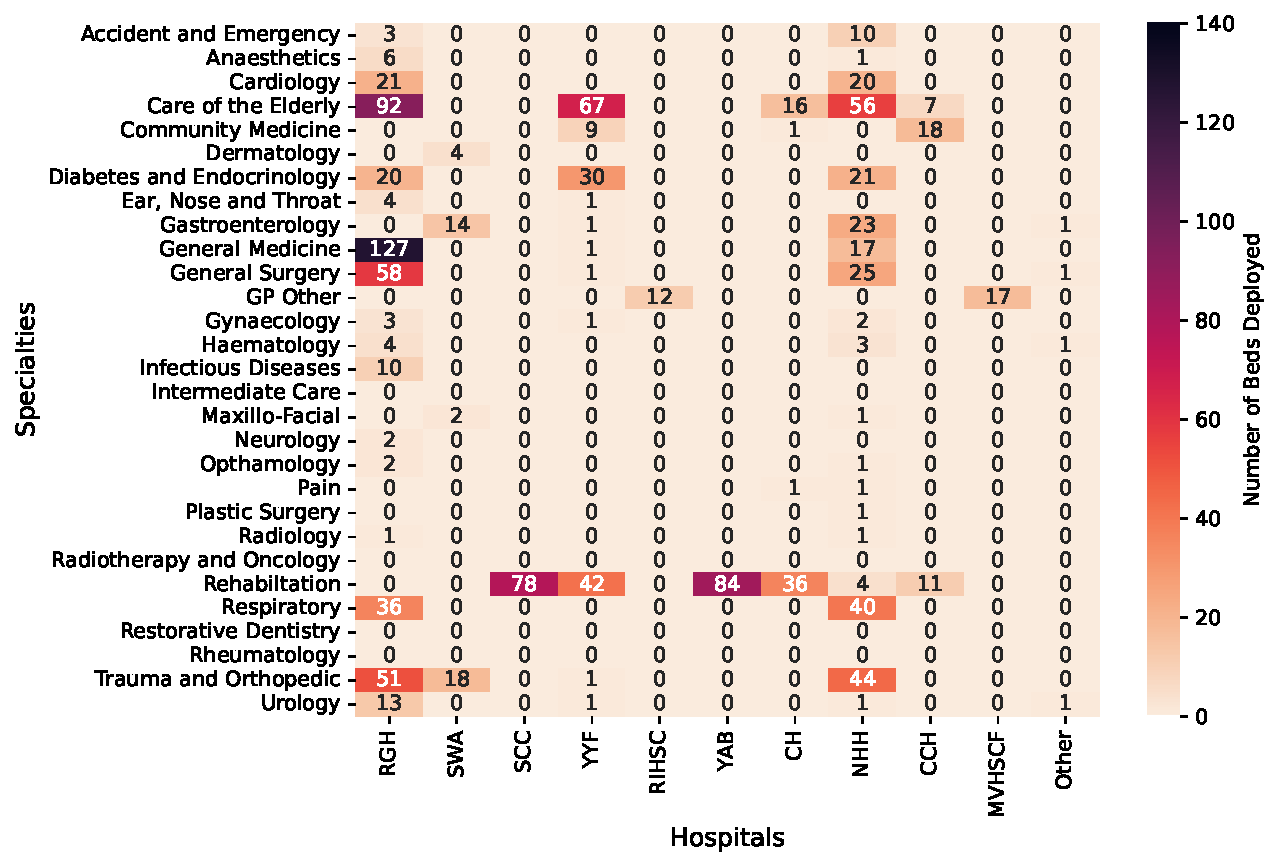
\includegraphics[scale=0.4]{Figures - Heatmaps/Fig40.pdf}  \captionsetup{font={scriptsize}}
  \captionof{figure}{Heatmap of bed locations for each specialty within each\\ hospital for the two-stage stochastic model using the classification tree and \\specific LOS for 2017-2018.}
  \label{fig:app22b}
\end{minipage}
\end{figure}

\begin{figure}[h!]
\centering
\begin{minipage}{0.4\linewidth}
  \centering
  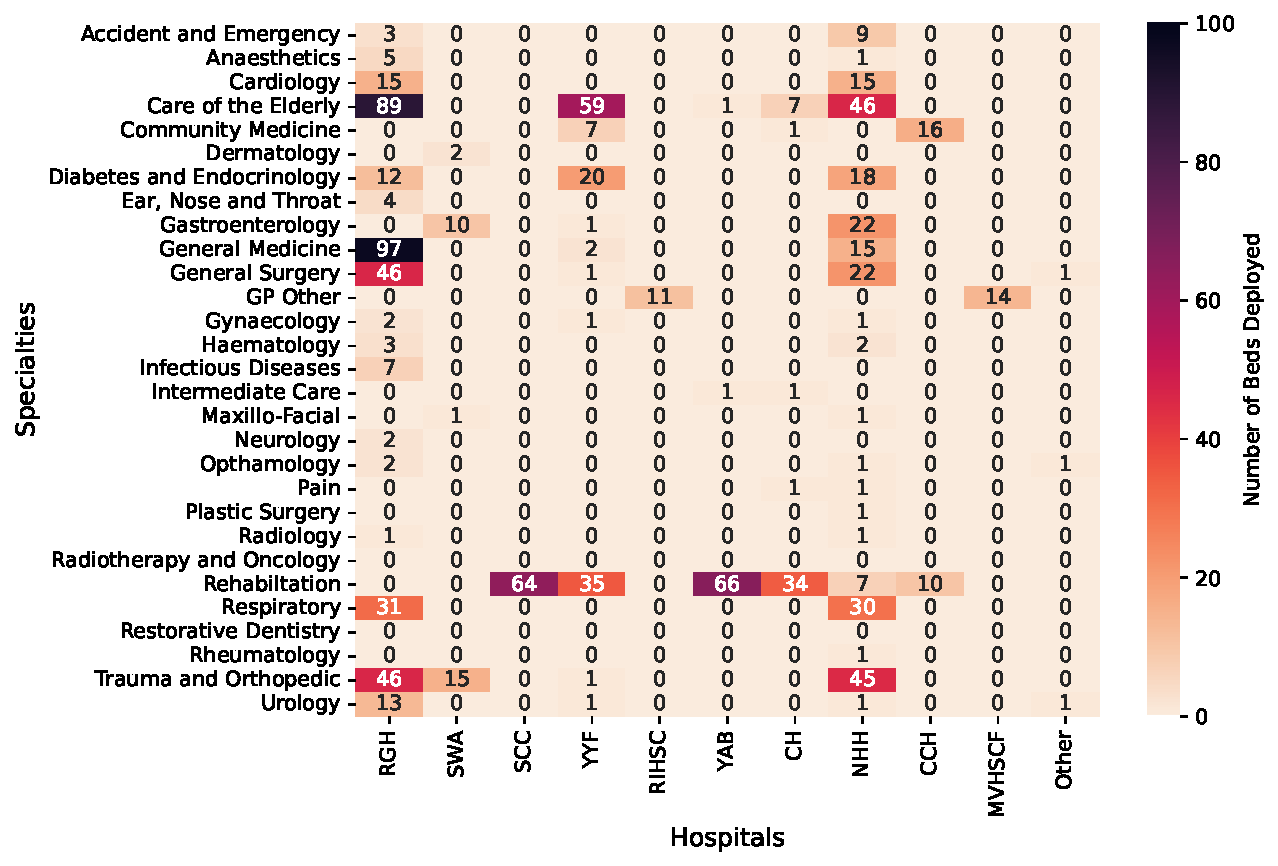
\includegraphics[scale=0.4]{Figures - Heatmaps/Fig41.pdf}
\captionsetup{font={scriptsize}}
  \captionof{figure}{{Heatmap of bed locations for each specialty within each\\ hospital for the deterministic model using the classification tree and \\specific LOS for 2018-2019.}}
  \label{fig:app23a}
\end{minipage}%
\begin{minipage}{0.4\linewidth}
  \centering
  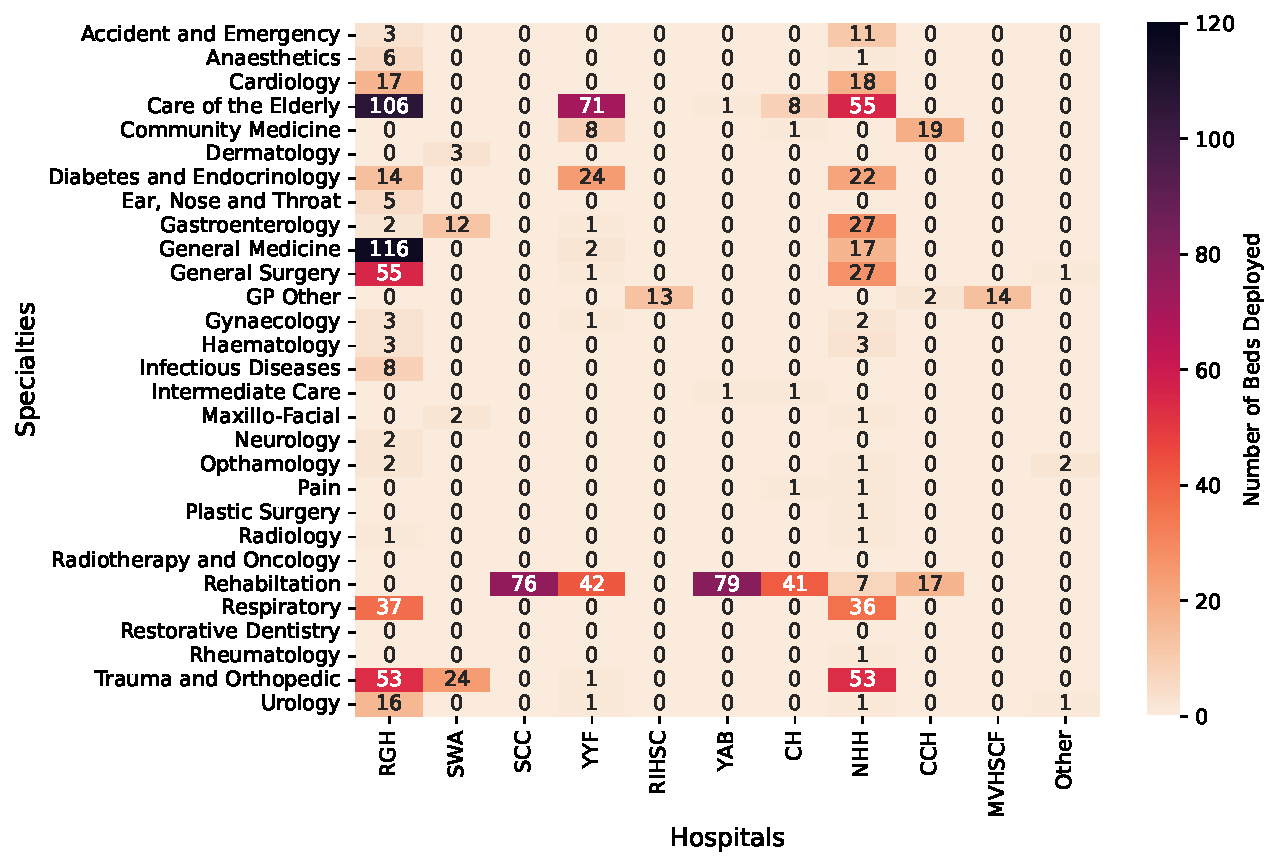
\includegraphics[scale=0.4]{Figures - Heatmaps/Fig42.pdf}
  \captionsetup{font={scriptsize}}
  \captionof{figure}{Heatmap of bed locations for each specialty within each\\ hospital for the two-stage stochastic model using the classification tree and \\specific LOS for 2018-2019.}
  \label{fig:app23b}
\end{minipage}
\end{figure}

\begin{figure}[h!]
\centering
\begin{minipage}{0.4\linewidth}
  \centering
  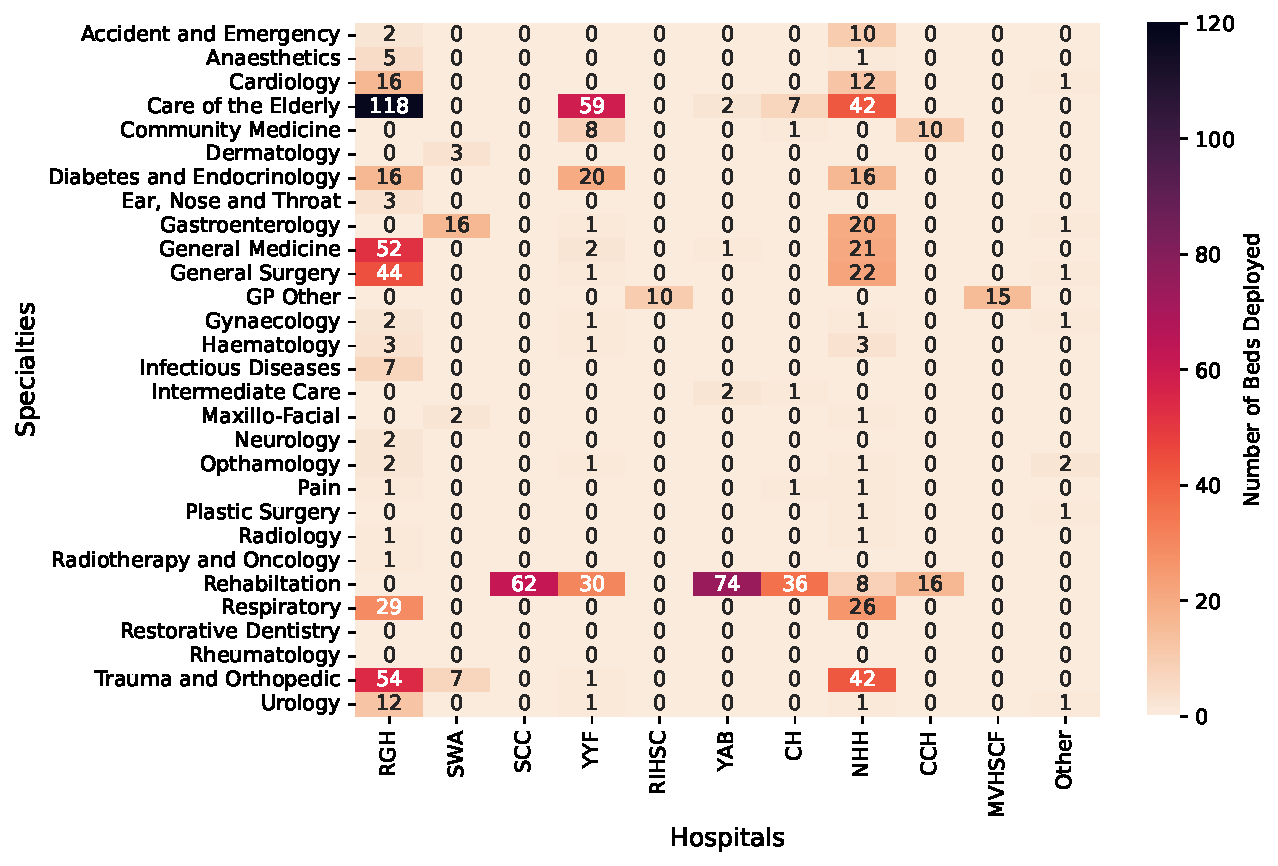
\includegraphics[scale=0.4]{Figures - Heatmaps/Fig43.pdf}
\captionsetup{font={scriptsize}}
  \captionof{figure}{Heatmap of bed locations for each specialty within each\\ hospital for the deterministic model using the classification tree and \\specific LOS for 2019-2020.}
  \label{fig:app24a}
\end{minipage}%
\begin{minipage}{0.4\linewidth}
  \centering
  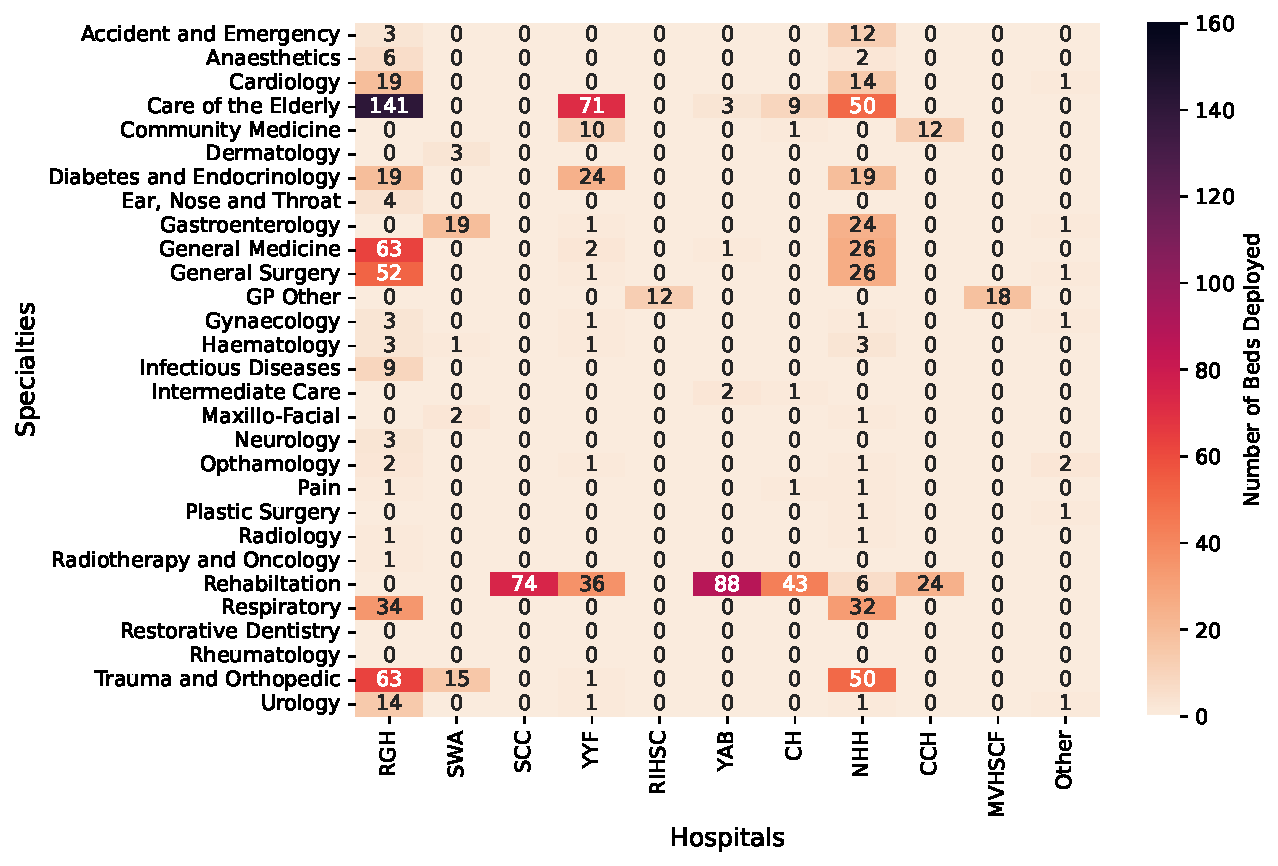
\includegraphics[scale=0.4]{Figures - Heatmaps/Fig44.pdf}
  \captionsetup{font={scriptsize}}
  \captionof{figure}{Heatmap of bed locations for each specialty within each\\ hospital for the two-stage stochastic model using the classification tree and \\specific LOS for 2019-2020.}
  \label{fig:app24b}
\end{minipage}
\end{figure}
\end{landscape}
\begin{landscape}
    
% \section{Scenario Analysis Data}
% This section contains the data used within the scenario analysis in Chapter \ref{sec:scenarioanalysis}.

% {\footnotesize
% \begin{longtable}{lp{17cm}}
% \label{tab:appscenariodata}
% \captionsetup{singlelinecheck=false}
% \caption{Data and Parameters Used within Scenario 1}\hline
% \textbf{Parameter} & \textbf{Two-Stage Stochastic Parameters} \\ \midrule
% Bands ($\mathcal{B})$ & b = [band5, band6, band7]\\  \midrule
% Specialties ($\mathcal{S})$ & s = [Accident and Emergency, Anaesthetics, Cardiology, Care of the Elderly, Community Medicine, Dermatology, Diabetes and Endocrinology, Ear, Nose and Throat, Gastroenterology, General Medicine, General Surgery, GP Other, Gynaecology, Haematology, Infectious Diseases, Intermediate Care, Maxillo-Facial, Neurology, Ophthalmology, Pain, Plastic Surgery, Radiology, Radiotherapy and Oncology, Rehabilitation, Respiratory, Restorative Dentistry, Rheumatology, Trauma and Orthopaedic, Urology]\\\midrule
% Hospitals ($\mathcal{H}$) & h = [Royal Gwent Hospital, St Woolos Acute Hospital, St Woolos Community Hospital, Ysbyty Ystrad Fawr, Rhymney Integrated Health and Social Care Centre, Ysbyty Aneurin Bevan, Grange University Hospital, County Hospital, Nevill Hall Hospital, Chepstow Community Hospital, Monnow Vale Integrated Health and Social Care Centre, University Hospital of Wales, Offsite, Outsource, Outsource - CareUK] \\\midrule
% Regions ($\mathcal{R}$) & r = [Region1, Region2, Region3, Region4, Region5, Region6]\\\midrule
% Scenarios ($\mathcal{S}$) & s = [Scenario1, Scenario2, Scenario3, Scenario 4]\\\midrule
% p$_{k}$ & [0.25, 0.25, 0.25, 0.25] \\\midrule
% c$^\textnormal{staff, 1st}_{b}$ & [$\pounds$338.88,	$\pounds$419.52, $\pounds$516.96]\\\midrule
% c$^\textnormal{staff, 2nd}_{b}$ & [$\pounds$454.80,	$\pounds$560.64, $\pounds$658.08] \\\midrule
% $UB^\textnormal{max, bed, 1st}_{h}$ & [297, 28, 75, 163, 12, 77, 300, 73, 171, 26, 16, 20, 20, 20 20]	   \\\midrule
% $UB^\textnormal{max, bed, 2nd}_{h}$ & [90, 9, 23, 49, 4, 24, 90, 22, 93, 8, 5, 6, 6, 6, 6]	   \\\hline
     
%  c$^\textnormal{bed, 1st}_{s,h}$ & $\begin{bmatrix}
% 0&	0&	0&	0&	0&	0&	247&	0&	0&	0&	0&	0\\
% 0&	0&	0&	0&	0&	0&	1021&	0&	0&	0&	0&	0\\
% 396&	0&	0&	0&	0&	0&	557&	0&	895&	0&	0&	0\\
% 457&	0&	755&	493&	0&	542&	577&	472&	743&	0&	0&	0\\
% 0&	0&	0&	942&	0&	0&	0&	1100&	0&	1021&	0&	0\\
% 0&	1381&	0&	0&	0&	0&	0&	0&	0&	0&	0&	0\\
% 296&	0&	0&	1021&	0&	0&	1270&	0&	1497&	0&	0&	0\\
% 481&	0&	0&	501&	0&	0&	481&	0&	501&	0&	0&	0\\
% 448&	0&	0&	639&	0&	0&	402&	0&	959&	0&	0&	832\\
% 390&	0&	0&	94&	0&	65&	290&	0&	611&	0&	0&	0\\
% 472&	0&	0&	304&	0&	0&	849&	0&	539&	0&	0&	0\\
% 0&	0&	0&	0&	183&	0&	0&	0&	0&	0&	448&	0\\
% 1007&	0&	0&	528&	0&	0&	517&	0&	292&	0&	0&	241\\
% 1299&	0&	0&	0&	0&	0&	1255&	0&	1070&	0&	0&	0\\
% 711&	0&	0&	0&	0&	0&	0&	0&	0&	0&	0&	0\\
% 0&	0&	0&	0&	0&	39&	0&	197&	0&	0&	0&	0\\
% 2026&	0&	0&	0&	0&	0&	1334&	0&	264&	0&	0&	0\\
% 711&	0&	0&	0&	0&	0&	0&	0&	0&	0&	0&	0\\
% 957&	0&	0&	369&	0&	0&	729&	0&	1416&	0&	0&	174\\
% 124&	0&	0&	111&	0&	0&	0&	134&	143&	0&	0&	0\\
% 0&	0&	0&	0&	0&	0&	0&	0&	0&	0&	0&	902\\
% 945&	0&	0&	0&	0&	0&	1021&	0&	1097&	0&	0&	0\\
% 0&	0&	0&	0&	0&	0&	0&	0&	0&	0&	0&	1089\\
% 1973&	0&	972&	975&	0&	1021&	1274&	1983&	1987&	1455&	0&	0\\
% 330&	0&	0&	448&	0&	0&	448&	0&	566&	0&	0&	0\\
% 120&	0&	0&	0&	0&	0&	0&	0&	0&	0&	0&	0\\
% 0&	0&	0&	0&	0&	0&	0&	0&	596&	0&	0&	0\\
% 678&	651&	0&	610&	0&	0&	703&	0&	873&	0&	0&	0\\
% 102&	0&	0&	0&	0&	0&	140&	0&	374&	0&	0&	900\\


% \end{bmatrix}$ \\\hline
%  c$^\textnormal{bed, 2nd}_{s,h}$ & $\begin{bmatrix}
% 0&	0&	0&	0&	0&	0&	296.4&	0&	0&	0&	0&	0\\
% 0&	0&	0&	0&	0&	0&	1225.2&	0&	0&	0&	0&	0\\
% 475.2	&0	&0	&0	&0	&0&	668.4&0	&1074&0	&0	&0\\
% 548.4	&0	&906&	591.6&	0&	650.4&	692.4	&566.4&	891.6&0&	0&	0\\
% 0&	0&	0&	1130.4	&0	&0	&0	&1320&	0	&1225.2&	0&0\\
% 0&	1657.2&0	&0	&0	&0	&0	&0&	0&	0	&0	&0\\
% 355.2	&0&	0	&1225.2&	0	&0&	1524&	0&1796.4&0&	0&0\\
% 577.2	&0	&0&	601.2&	0	&0	&577.2	&0	&601.2	&0	&0	&0\\
% 537.6	&0	&0	&766.8&	0	&0	&482.4	&0	&1150.8	&0&	0	&998.4\\
% 468&	0	&0	&112.8&	0&	78&	348&	0&	733.2&	0	&0	&0\\
% 566.4	&0	&0&	364.8&	0&	0	&1018.8	&0	&646.8&	0&	0	&0\\
% 0	&0	&0&0	&219.6&	0&0	&0	&0&	0&	537.6&	0\\
% 1208.4	&0&	0	&633.6	&0&	0	&620.4	&0	&350.4&0	&0	&289.2\\
% 1558.8	&0&	0&	0&	0&	0&	1506&	0&	1284&	0&	0&	0\\
% 853.2	&0&	0&	0&	0&	0&	0&	0&	0&	0&	0&	0\\
% 0	&0	&0&	0&	0	&46.8	&0&	236.4	&0&0	&0	&0\\
% 2431.2	&0	&0	&0	&0	&0	&1600.8&	0&	316.8&	0&	0&	0\\
% 853.2	&0	&0	&0	&0&	0	&0	&0&0	&0	&0&	0\\
% 1148.4&	0	&0	&442.8&	0	&0	&874.8	&0	&1699.2	&0	&0&	208.8\\
% 148.8	&0&	0	&133.2&	0&	0	&0	&160.8	&171.6&0	&0&	0\\
% 0&0	&0	&0&	0	&0&0	&0&	0&	0&	0&	1082.4\\
% 1134&	0&	0	&0	&0&	0&	1225.2&	0&	1316.4&	0&	0&	0\\
% 0	&0&	0&	0	&0	&0&	0&	0&	0	&0&	0	&1306.8\\
% 2367.6	&0	&1166.4&	1170&	0	&1225.2	&1528.8&	2379.6&	2384.4&1746&	0&	0\\
% 396&	0	&0	537.6&	0&	0&	537.6&	0&	679.2&	0&	0&	0\\
% 144&	0	&0	&0&	0	&0	&0	&0&	0&	0	&0	&0\\
% 0	&0&	0	&0	&0	&0	&0	&0&	715.2	&0	&0&	0\\
% 813.6	&781.2	&0	&732	&0	&0	&843.6&	0&1047.6	&0&	0&	0\\
% 122.4	&0	&0	&0	&0	&0&168	&0&	448.8	&0&0&1080\\
% \end{bmatrix}$\\\hline
%         R$_{s,b}$ & 
%         $\begin{bmatrix}
%             0.250 &	0.25 &	0.25& \\
%             0.250 &	0.25 &	0.25& \\
%             0.125 &	0.125 &	0.125& \\
%             0.1 &	0.1 &	0.1& \\
%             0.1 &	0.1 &	0.1& \\
%             0.1 &	0.1 &	0.1& \\
%             0.125 &	0.125 &	0.125& \\
%             0.125 &	0.125 &	0.125& \\
%             0.125 &	0.125 &	0.125& \\
%             0.25 &	0.25 &	0.25& \\
%             0.25 &	0.25 &	0.25& \\
%             0.1 &	0.1 &	0.1& \\
%             0.125 &	0.125 &	0.125& \\
%             0.125 &	0.125 &	0.125& \\
%             0.125 &	0.125 &	0.125& \\
%             0.1 &	0.1 &	0.1& \\
%             0.125 &	0.125 &	0.125& \\
%             0.125 &	0.125 &	0.125& \\
%             0.125 &	0.125 &	0.125& \\
%             0.125 &	0.125 &	0.125& \\
%             0.125 &	0.125 &	0.125& \\
%             0.125 &	0.125 &	0.125& \\
%             0.125 &	0.125 &	0.125& \\
%             0.1 &	0.1 &	0.1& \\
%             0.125 &	0.125 &	0.125& \\
%             0.125 &	0.125 &	0.125& \\
%             0.125 &	0.125 &	0.125& \\
%             0.25 &	0.25 &	0.25& \\
%             0.125 &	0.125 &	0.125& \\

%         \end{bmatrix}$ \\\hline
%         $K_{s,h}$ & $\begin{bmatrix}
            
% 0&	0&	0	&0&	0&	0&	300&	0&	0&	0&	0&	0\\
% 0&	0&	0	&0&	0&	0&	300&	0&	0&	0&	0&	0\\
% 297&	0&	0	&163&	0&	0&	300&	0&	171&	0&	0&	0\\
% 297&	0&	75	&163&	0&	77&	300&	73&	171&	0&	0&	0\\
% 0&	0&	0	&163&	0&	0&	0&	73&	0&	26&	0&	0\\
% 0&	28&	0	&0&	0&	0&	0&	0&	0&	0&	0&	0\\
% 297&	0&	0	&163&	0&	0&	300&	0&	171&	0&	0&	0\\
% 297&	0&	0	&163&	0&	0&	300&	0&	171&	0&	0&	0\\
% 297&	0&	0	&163&	0&	0&	300&	0&	171&	0&	0&	80\\
% 297&	0&	0	&163&	0&	77&	300&	0&	171&	0&	0&	0\\
% 297&	0&	0	&163&	0&	0&	300&	0&	171&	0&	0&	0\\
% 0&	0&	0	&0&	12&	0&	0&	0&	0&	0&	16&	0\\
% 297&	0&	0	&163&	0&	0&	300&	0&	171&	0&	0&	80\\
% 297&	0&	0	&0&	0&	0&	300&	0&	171&	0&	0&	0\\
% 297&	0&	0	&0&	0&	0&	0&	0&	0&	0&	0&	0\\
% 0&	0&	0	&0&	0&	77&	0&	73&	0&	0&	0&	0\\
% 297&	0&	0	&0&	0&	0&	300&	0&	171&	0&	0&	0\\
% 297&	0&	0	&0&	0&	0&	0&	0&	0&	0&	0&	0\\
% 297&	0&	0	&163&	0&	0&	300&	0&	171&	0&	0&	80\\
% 297&	0&	0	&163&	0&	0&	0&	73&	171&	0&	0&	0\\
% 0&	0&	0	&0&	0&	0&	0&	0&	0&	0&	0&	80\\
% 297&	0&	0	&0&	0&	0&	300&	0&	171&	0&	0&	0\\
% 0&	0&	0	&0&	0&	0&	0&	0&	0&	0&	0&	80\\
% 297&	0&	75	&163&	0&	77&	300&	73&	171&	26&	0&	0\\
% 297&	0&	0	&163&	0&	0&	300&	0&	171&	0&	0&	0\\
% 297&	0&	0	&0&	0&	0&	0&	0&	0&	0&	0&	0\\
% 0&	0&	0	&0&	0&	0&	0&	0&	171&	0&	0&	0\\
% 297&	28&	0	&163&	0&	0&	300&	0&	171&	0&	0&	0\\
% 297&	0&	0	&0&	0&	0&	300&	0&	171&	0&	0&	80
% \end{bmatrix}$\\\bottomrule
% \end{longtable}

\section{Scenario Heatmaps}
This section contains the heatmaps produced from performing various scenario analysis within Chapter \ref{sec:scenarioanalysis}.

    

\begin{figure}[h!]
\centering
\begin{minipage}{0.4\linewidth}
  \centering
  \includegraphics[scale=0.4]{Figures - Heatmaps/Fig45.pdf}
  \captionsetup{font={scriptsize}}
  \captionof{figure}{{Heatmap of bed locations for each specialty within each\\ hospital for the deterministic model for Scenario 1 where GUH is added.}}
  \label{fig:dets1}
\end{minipage}%
\begin{minipage}{0.4\linewidth}
  \centering
  \includegraphics[scale=0.4]{Figures - Heatmaps/Fig46.pdf}  \captionsetup{font={scriptsize}}
   \captionof{figure}{{Heatmap of bed locations for each specialty within each\\ hospital for the two-stage stochastic model for Scenario 1 where GUH is added.}}
  \label{fig:stocs2}
\end{minipage}
\end{figure}

\begin{figure}[h!]
\centering
\begin{minipage}{0.4\linewidth}
  \centering
  \includegraphics[scale=0.4]{Figures - Heatmaps/Fig47.pdf}
\captionsetup{font={scriptsize}}
  \captionof{figure}{{Heatmap of bed locations for each specialty within each\\ hospital for the deterministic model for Scenario 2 where the\\ M-penalty method is added.}}
  \label{fig:dets2}
\end{minipage}%
\begin{minipage}{0.4\linewidth}
  \centering
  \includegraphics[scale=0.4]{Figures - Heatmaps/Fig48.pdf}
  \captionsetup{font={scriptsize}}
  \captionof{figure}{{Heatmap of bed locations for each specialty within each\\ hospital for the two-stage stochastic model for Scenario 2 where the\\ M-penalty method is added.}}
  \label{fig:stochs2}
\end{minipage}
\end{figure}

\begin{figure}[h!]
\centering
\begin{minipage}{0.4\linewidth}
  \centering
  \includegraphics[scale=0.4]{Figures - Heatmaps/Fig49.pdf}
\captionsetup{font={scriptsize}}
  \captionof{figure}{{Heatmap of bed locations for each specialty within each\\ hospital for the deterministic model for Scenario 3 where the\\ hospital setup is re-evaluated.}}
  \label{fig:dets3}
\end{minipage}%
\begin{minipage}{0.4\linewidth}
  \centering
  \includegraphics[scale=0.4]{Figures - Heatmaps/Fig50.pdf}
  \captionsetup{font={scriptsize}}
  \captionof{figure}{{Heatmap of bed locations for each specialty within each\\ hospital for the two-stage stochastic model for Scenario 3 where the\\ hospital setup is re-evaluated.}}
  \label{fig:stochs3}
\end{minipage}
\end{figure}

\begin{figure}[h!]
\centering
\begin{minipage}{0.4\linewidth}
  \centering
  \includegraphics[scale=0.4]{Figures - Heatmaps/Fig51.pdf}
\captionsetup{font={scriptsize}}
  \captionof{figure}{{Heatmap of bed locations for each specialty within each\\ hospital for the deterministic model for Scenario 4 where the\\ nursing capacity is reduced.}}
  \label{fig:dets4}
\end{minipage}%
\begin{minipage}{0.4\linewidth}
  \centering
  \includegraphics[scale=0.4]{Figures - Heatmaps/Fig52.pdf}
  \captionsetup{font={scriptsize}}
  \captionof{figure}{{Heatmap of bed locations for each specialty within each\\ hospital for the two-stage stochastic model for Scenario 4 where the\\ nursing capacity is reduced.}}
  \label{fig:stochs4}
\end{minipage}
\end{figure}
\begin{figure}[h!]
\centering
\begin{minipage}{0.4\linewidth}
  \centering
  \includegraphics[scale=0.4]{Figures - Heatmaps/Fig53.pdf}
\captionsetup{font={scriptsize}}
  \captionof{figure}{{Heatmap of bed locations for each specialty within each\\ hospital for the deterministic model for Scenario 5 with the\\ introduction of virtual wards.}}
  \label{fig:dets5}
\end{minipage}%
\begin{minipage}{0.4\linewidth}
  \centering
  \includegraphics[scale=0.4]{Figures - Heatmaps/Fig54.pdf}
  \captionsetup{font={scriptsize}}
  \captionof{figure}{{Heatmap of bed locations for each specialty within each\\ hospital for the two-stage stochastic model for Scenario 5 with the\\ introduction of virtual wards.}}
  \label{fig:stochs5}
\end{minipage}
\end{figure}
\begin{figure}[h!]
\centering
\begin{minipage}{0.4\linewidth}
  \centering
  \includegraphics[scale=0.4]{Figures - Heatmaps/Fig55.pdf}
\captionsetup{font={scriptsize}}
  \captionof{figure}{{Heatmap of bed locations for each specialty within each\\ hospital for the deterministic model for Scenario 6 with the\\ sudden increase in demand.}}
  \label{fig:dets6}
\end{minipage}%
\begin{minipage}{0.4\linewidth}
  \centering
  \includegraphics[scale=0.4]{Figures - Heatmaps/Fig56.pdf}
  \captionsetup{font={scriptsize}}
  \captionof{figure}{{Heatmap of bed locations for each specialty within each\\ hospital for the two-stage model for Scenario 6 with the\\ sudden increase in demand.}}
  \label{fig:stochs6}
\end{minipage}
\end{figure}


\begin{figure}[h!]
\centering
\begin{minipage}{0.4\linewidth}
  \centering
  \includegraphics[scale=0.4]{Figures - Heatmaps/Fig57.pdf}
\captionsetup{font={scriptsize}}
  \captionof{figure}{{Heatmap of bed locations for each specialty within each\\ hospital for the deterministic model for Scenario 7 with an\\ overall increase in T\&O services of 10\%.}}
  \label{fig:dets6}
\end{minipage}%
\begin{minipage}{0.4\linewidth}
  \centering
  \includegraphics[scale=0.4]{Figures - Heatmaps/Fig58.pdf}
  \captionsetup{font={scriptsize}}
  \captionof{figure}{{Heatmap of bed locations for each specialty within each\\ hospital for the two-stage stochastic model for Scenario 7 with an\\ overall increase in T\&O services of 10\%.}}
  \label{fig:stochs6}
\end{minipage}
\end{figure}

\begin{figure}[h!]
\centering
\begin{minipage}{0.4\linewidth}
  \centering
  \includegraphics[scale=0.4]{Figures - Heatmaps/Fig59.pdf}
\captionsetup{font={scriptsize}}
  \captionof{figure}{{Heatmap of bed locations for each specialty within each\\ hospital for the deterministic model for Scenario 7 with targetting\\ T\&O specific nodes in the regression tree with a 10\% increase.}}
  \label{fig:dets6}
\end{minipage}%
\begin{minipage}{0.4\linewidth}
  \centering
  \includegraphics[scale=0.4]{Figures - Heatmaps/Fig60.pdf}
  \captionsetup{font={scriptsize}}
  \captionof{figure}{{Heatmap of bed locations for each specialty within each\\ hospital for the two-stage stochastic model for Scenario 7 with targetting\\ T\&O specific nodes in the regression tree with a 10\% increase.}}
  \label{fig:stochs6}
\end{minipage}
\end{figure}

\end{landscape}



\end{document}